% **************************************************
% Document Class Definition
% **************************************************
\documentclass[%
	paper=A4,					% paper size --> A4 is default in Germany
	twoside=true,				% onesite or twoside printing
	openright,					% doublepage cleaning ends up right side
	parskip=full,				% spacing value / method for paragraphs
	chapterprefix=true,			% prefix for chapter marks
	11pt,						% font size
	headings=normal,			% size of headings
	bibliography=totoc,			% include bib in toc
	listof=totoc,				% include listof entries in toc
	titlepage=on,				% own page for each title page
	captions=tableabove,		% display table captions above the float env
	draft=false,				% value for draft version
]{scrreprt}%

% **************************************************
% Debug LaTeX Information
% **************************************************
%\listfiles

% **************************************************
% Information and Commands for Reuse
% **************************************************
\newcommand{\thesisTitle}{The Clean Thesis Style}
\newcommand{\thesisName}{Ricardo Langner}
\newcommand{\thesisSubject}{Documentation}
\newcommand{\thesisDate}{August 26, 2015}
\newcommand{\thesisVersion}{My First Draft}

\newcommand{\thesisFirstReviewer}{Jane Doe}
\newcommand{\thesisFirstReviewerUniversity}{\protect{Clean Thesis Style University}}
\newcommand{\thesisFirstReviewerDepartment}{Department of Clean Thesis Style}

\newcommand{\thesisSecondReviewer}{John Doe}
\newcommand{\thesisSecondReviewerUniversity}{\protect{Clean Thesis Style University}}
\newcommand{\thesisSecondReviewerDepartment}{Department of Clean Thesis Style}

\newcommand{\thesisFirstSupervisor}{Jane Doe}
\newcommand{\thesisSecondSupervisor}{John Smith}

\newcommand{\thesisUniversity}{\protect{Clean Thesis Style University}}
\newcommand{\thesisUniversityDepartment}{Department of Clean Thesis Style}
\newcommand{\thesisUniversityInstitute}{Institut for Clean Thesis Dev}
\newcommand{\thesisUniversityGroup}{Clean Thesis Group (CTG)}
\newcommand{\thesisUniversityCity}{City}
\newcommand{\thesisUniversityStreetAddress}{Street address}
\newcommand{\thesisUniversityPostalCode}{Postal Code}

\newcommand{\forcenewpage}{\clearpage \newpage \mbox{~} \clearpage \newpage}

% --------------------------
% new commands
% --------------------------
\newcommand{\CC}{\ensuremath{\mathbb{C}} }
\newcommand{\NN}{\ensuremath{\mathbb{N}} }
\newcommand{\RR}{\ensuremath{\mathbb{R}} }
\newcommand{\QQ}{\ensuremath{\mathbb{Q}} }
\newcommand{\EE}{\ensuremath{\mathbb{E}} }
\newcommand{\PP}{\ensuremath{\mathbb{P}} }
\newcommand{\noi}{\noindent}
\newcommand{\II}{\mbox{\large 1\hskip -0,353em 1}}
\newcommand{\dps}{\displaystyle}
\newcommand{\ms}{\medskip}
\newcommand{\itb}{\ms\item[$\bullet$]}
\newcommand{\itm}{\ms\item}
\newcommand{\pkg}[1]{{\normalfont\fontseries{b}\selectfont #1}}
\newcommand{\proglang}[1]{\textsf{#1}}
\newcommand{\code}[1]{\mbox{\texttt{#1}}}
\newcommand{\MN}{\mathcal{N}}
\newcommand{\MM}{\mathcal{M}}
\newcommand{\FF}{\mathcal{F}}
\newcommand{\GG}{\mathcal{G}}
\newcommand{\HH}{\mathcal{H}}
\newcommand{\LL}{\mathcal{L}}
\newcommand{\AT}{\mathcal{A}}
\newcommand{\bfX}{{\bf X}}
\newcommand{\bfY}{{\bf Y}}


% **************************************************
% Load and Configure Packages
% **************************************************
\usepackage[utf8]{inputenc}		% defines file's character encoding
\usepackage[english]{babel} % babel system, adjust the language of the content
\usepackage[					% clean thesis style
	figuresep=colon,%
	sansserif=false,%
	hangfigurecaption=false,%
	hangsection=true,%
	hangsubsection=true,%
	colorize=full,%
	colortheme=bluemagenta,%
	bibsys=bibtex,%
	bibfile=bib-refs,%
	bibstyle=alphabetic,%
]{cleanthesis}

% --------------------------
% packages
% --------------------------
\usepackage{amssymb,amsfonts,amsmath, bm}

\usepackage{graphicx}

\def\proof{\noindent \textbf{\emph{\textbf{Proof}.$\,$}}}
\def\finproof {\hfill $\Box$ \vskip 5 pt }


\hypersetup{					% setup the hyperref-package options
	pdftitle={\thesisTitle},	% 	- title (PDF meta)
	pdfsubject={\thesisSubject},% 	- subject (PDF meta)
	pdfauthor={\thesisName},	% 	- author (PDF meta)
	plainpages=false,			% 	-
	colorlinks=false,			% 	- colorize links?
	pdfborder={0 0 0},			% 	-
	breaklinks=true,			% 	- allow line break inside links
	bookmarksnumbered=true,		%
	bookmarksopen=true			%
}

% **************************************************
% Document CONTENT
% **************************************************
\begin{document}

% --------------------------
% rename document parts
% --------------------------
%\renewcaptionname{ngerman}{\figurename}{Abb.}
%\renewcaptionname{ngerman}{\tablename}{Tab.}
\renewcaptionname{english}{\figurename}{Fig.}
\renewcaptionname{english}{\tablename}{Tab.}

% --------------------------
% Front matter
% --------------------------
\pagenumbering{roman}			% roman page numbing (invisible for empty page style)
\pagestyle{empty}				% no header or footers
% !TEX root = ../thesis-example.tex
%
% ------------------------------------  --> cover title page
\begin{titlepage}
\setlength{\parindent}{0pt}
\thispagestyle{empty}


\begin{center}

\includegraphics[height=1.75cm]{gfx/logo}
\end{center}


\fontsize{10pt}{12pt}\selectfont
N\textsuperscript{o} d'ordre NNT : xxx

\vspace{0.1cm}

\begin{center}
\fontsize{13pt}{15pt}\selectfont
\textbf{\uppercase{Thèse de doctorat de l'universit\'e de Lyon}}\\
\fontsize{11pt}{13pt}\selectfont
oper\'ee au sein de\\
\textbf{l'Universit\'e Claude Bernard Lyon 1}

\vspace{0.2cm}

\textbf{Ecole Doctorale ED SEG\\% rectifier le numero d'accreditation
EA n°2429}% nom complet de l'ecole doctorale

\vspace{0.1cm}

\textbf{Specialit\'e de doctorat : Actuariat\\
Discipline : Sciences de Gestion} % eventuellement

\vspace{0.1cm}

Soutenue publiquement le 05/07/2018, par :\\
\fontsize{14pt}{16pt}\selectfont
\textbf{Thierry Moudiki Ndoumbe}

\vspace{0.1cm} % adapter à la longueur du titre

\rule[20pt]{\textwidth}{0.5pt}

\fontsize{20pt}{25pt}\selectfont
\textbf{Interest rates modeling for insurance - interpolation, extrapolation, and forecasting}

\rule{\textwidth}{0.5pt}

\vspace{0.1cm} % adapter à la longueur du titre
\end{center}

\fontsize{11pt}{13pt}\selectfont
Devant le jury compos\'e de :
\medskip

\fontsize{9pt}{11pt}\selectfont

Nom Prenom, grade/qualit\'e, \'etablissement/entreprise \hfill Pr\'esident(e)

\medskip

Franck Moraux, Professeur des universit\'es, Universit\'e de Rennes I \hfill  Rapporteur(e)

Donatien Hainaut,  Professeur des universit\'es, Universit\'e Catholique de Louvain \hfill Rapporteur(e)

Diana Dorobantu, Maitre de Conf\'erences, ISFA, Universit\'e Lyon I \hfill Examinatrice

Armelle Guillou, Professeure des universit\'es, Universit\'e de Strasbourg \hfill Examinatrice

Florence Picard, Pr\'esidente de la commission scientifique, Institut des actuaires \hfill Examinatrice

St\'ephane Loisel, Professeur des universit\'es, ISFA, Universit\'e Lyon I \hfill Examinateur/trice

\medskip

Fr\'ed\'eric Planchet, Professeur des universit\'es, ISFA, Universit\'e Lyon I \hfill Directeur de thèse

Areski Cousin, Professeur des universit\'es, Universit\'e de Strasbourg \hfill Co-directeur de thèse % le cas echeant

\newpage
%\fontsize{12pt}{14pt}\selectfont   % si le document general n'est pas en police 11pt, decommenter et preciser la taille utilisee
% Suite du manuscrit
\end{titlepage}


% ------------------------------------  --> main title page
% \begin{titlepage}
% 	\pdfbookmark[0]{Titlepage}{Titlepage}
% 	\tgherosfont
% 	\centering
%
% 	{\Large \thesisUniversity} \\[4mm]
% 	
\includegraphics[width=6cm]{gfx/Clean-Thesis-Logo} \\[2mm]
% 	\textsf{\thesisUniversityDepartment} \\
% 	\textsf{\thesisUniversityInstitute} \\
% 	\textsf{\thesisUniversityGroup} \\
%
% 	\vfill
% 	{\large \thesisSubject} \\[5mm]
% 	{\LARGE \color{ctcolortitle}\textbf{\thesisTitle} \\[10mm]}
% 	{\Large \thesisName} \\
%
% 	\vfill
% 	\begin{minipage}[t]{.27\textwidth}
% 		\raggedleft
% 		\textit{1. Reviewer}
% 	\end{minipage}
% 	\hspace*{15pt}
% 	\begin{minipage}[t]{.65\textwidth}
% 		{\Large \thesisFirstReviewer} \\
% 	  	{\small \thesisFirstReviewerDepartment} \\[-1mm]
% 		{\small \thesisFirstReviewerUniversity}
% 	\end{minipage} \\[5mm]
% 	\begin{minipage}[t]{.27\textwidth}
% 		\raggedleft
% 		\textit{2. Reviewer}
% 	\end{minipage}
% 	\hspace*{15pt}
% 	\begin{minipage}[t]{.65\textwidth}
% 		{\Large \thesisSecondReviewer} \\
% 	  	{\small \thesisSecondReviewerDepartment} \\[-1mm]
% 		{\small \thesisSecondReviewerUniversity}
% 	\end{minipage} \\[10mm]
% 	\begin{minipage}[t]{.27\textwidth}
% 		\raggedleft
% 		\textit{Supervisors}
% 	\end{minipage}
% 	\hspace*{15pt}
% 	\begin{minipage}[t]{.65\textwidth}
% 		\thesisFirstSupervisor\ and \thesisSecondSupervisor
% 	\end{minipage} \\[10mm]
%
% 	\thesisDate \\
%
% \end{titlepage}


% ------------------------------------  --> lower title back for single page layout
% \hfill
% \vfill
% {
% 	\small
% 	\textbf{\thesisName} \\
% 	\textit{\thesisTitle} \\
% 	\thesisSubject, \thesisDate \\
% 	Reviewers: \thesisFirstReviewer\ and \thesisSecondReviewer \\
% 	Supervisors: \thesisFirstSupervisor\ and \thesisSecondSupervisor \\[1.5em]
% 	\textbf{\thesisUniversity} \\
% 	\textit{\thesisUniversityGroup} \\
% 	\thesisUniversityInstitute \\
% 	\thesisUniversityDepartment \\
% 	\thesisUniversityStreetAddress \\
% 	\thesisUniversityPostalCode\ and \thesisUniversityCity
% }
		% INCLUDE: all titlepages
\cleardoublepage

\pagestyle{plain}				% display just page numbers
%% !TEX root = ../thesis-example.tex
%
\pdfbookmark[0]{Abstract}{Abstract}
\chapter*{Abstract}
\label{sec:abstract}
\vspace*{-10mm}

\blindtext

\vspace*{20mm}

{\usekomafont{chapter}Abstract (different language)}\label{sec:abstract-diff} \\

\blindtext
		% INCLUDE: the abstracts (english and german)
%\cleardoublepage
%
%% !TEX root = ../thesis-example.tex
%
\pdfbookmark[0]{Acknowledgement}{Acknowledgement}
\chapter*{Acknowledgement}
\label{sec:acknowledgement}
\vspace*{-10mm}

Thank you, to those who made this possible.
 % INCLUDE: acknowledgement
%\cleardoublepage
%
\setcounter{tocdepth}{2}		% define depth of toc
\tableofcontents				% display table of contents
\cleardoublepage

% --------------------------
% Body matter
% --------------------------
\pagenumbering{arabic}			% arabic page numbering
\setcounter{page}{1}			% set page counter
\pagestyle{maincontentstyle} 	% fancy header and footer

%% !TEX root = ../thesis-example.tex
%

\chapter{Introduction}
\label{sec:intro}

\section{Motivation and Problem Statement (French version)}

L'ORSA (Own Risk Solvency and Assessment) est un ensemble de règles définies par la directive européenne Solvabilit\'e II, destiné à servir d'outil d'aide à la décision et d'analyse stratégique des risques. Dans le cadre de l'ORSA, les compagnies d'assurance doivent évaluer leur solvabilité future de façon continue et prospective. Et pour ce faire, elles doivent notamment obtenir des projections probabilistes de leur bilan (actif et passif) sur un certain horizon temporel.   

Dans ce travail de thèse, nous nous focalisons sur l'actif; la prévision des valeurs futures des actifs. Nous traitons plus précisément des taux d'intérêts; de la construction, de l'extrapolation, et des prévisions envisagées dans le futur pour la courbe de taux d'intérêt. Les techniques présentées sont essentiellement basées sur des méthodes d'apprentissage statistique.    

Nous parlerons généralement dans le texte de \textit{courbe de taux}, mais il s'agit en fait  de courbes de facteurs d'actualisation sans risque de défaut de contrepartie. Le risque de défaut de contrepartie n'est pas explicitement traité, mais des techniques similaires à celles développées ici, peuvent être transposées à la construction de courbe de taux incorporant un risque de défaut de contrepartie.

Nous présentons dans un premier temps, une famille de courbes de facteurs d'actualisation basées sur les modèles de taux (courts) dits d'absence d'opportunité d'arbitrage ou exogènes. À une date donnée, la courbe d'actualisation est construite à l'aide de produits dérivés de taux, dont les cotations sont disponibles sur les marchés financiers pour un nombre donné de maturités. La régularité de la courbe obtenue est également paramétrable, en fonction du résultat recherché par l'utilisateur. Nous montrons comment cette courbe de facteurs d'actualisation, obtenue à une date donnée, peut être extrapolée au-delà des maturités disponibles sur les marchés, et comment les courbes construites à différentes dates dans le temps, peuvent être utilisées pour obtenir des prévisions de taux d'intérêts dans le futur.  Pour ce dernier point portant sur la prévision, des techniques basées sur l'\textbf{analyse en composantes principales (ACP) fonctionnelle} sont appliquées aux paramètres du modèle. 

Nous présentons ensuite un modèle de prévision simultanée de séries temporelles multivariées, basé sur des réseaux de neurones dits \textbf{Random Vector Functional Link (RVFL) networks}. Les RVFL ont été utilisés avec succès par le passé, pour des problèmes de régression, de classification, et de prévision de séries temporelles univariées. La nouveauté ici, est de les appliquer à des séries temporelles multivariées avec plusieurs contraintes de régularisation sur les paramètres, et des variables explicatives quasi-aléatoires. Les exemples d'application portent sur la prévision de courbes de facteurs d'actualisation. Le modèle ainsi obtenu est un modèle robuste, notamment grâce à ses paramètres de régularisation, et on montre qu'il obtient de très bonnes performances quand il est comparé à des modèles similaires. Il peut également être utilisé dans le cadre de \textit{stress tests}. 

Dans le chapitre 4, des méthodes d'apprentissage dites ensemblistes sont appliquées à la prévision simultanée de taux d'intérêts, avec d'autres variables macroéconomiques telles que l'inflation. Ces méthodes ensemblistes sont construites à partir de modèles relativement plus simples; et le modèle de base utilisé ici pour la construction des ensembles est le modèle RVFL. Trois types de méthodes ensemblistes sont envisagées: \textbf{bootstrap aggregating},  \textbf{boosting}, et \textbf{stacked generalization}. On observe ici, généralement, que ces méthodes ensemblistes peuvent permettre d'obtenir des améliorations de performance par rapport aux modèles de base qui les constituent. Il est à noter que cette amélioration ne sera pas observée de façon systématique sur d'autres jeux de données. Mais ce type de modèle aura toujours un intérêt à être envisagé dans une optique d'accroissement des performances prédictives. 

Le chapitre suivant étudie l'application des méthodes d'apprentissage basées sur des noyaux (\textbf{Kernel Regularized Least Squares}, KRLS) à la prévision de courbes de taux d'intérêt. Les modèles de type KRLS expriment la variable à expliquer (ici, le taux \textit{spot}) comme une combinaison linéaire de distances entre les observations des variables explicatives. Ces méthodes sont appliquées ici, d'abord dans le contexte populaire de Nelson-Siegel dynamique qui représente la courbe de taux en fonction de trois facteurs explicatifs, puis directement aux taux \textit{spot}. Cette deuxième approche s'apparentant à des approches appliquées en géostatistique, permet d'obtenir de bonnes performances de prévision, tout en reproduisant des faits stylisés de la courbe de taux sans contrainte de forme supplémentaire.

Le dernier chapitre compare les différents modèles introduits dans les chapitres précédents. Pour ce faire, il revisite le modèle RVFL introduit aux chapitre 3, en adjoignant à ses paramètres une distribution \textit{a priori} (Gaussienne multivariée). Le modèle ainsi obtenu sert d'ingrédient de base à une méthode d'optimisation bayésienne, appliquée à la minimisation de l'erreur de validation croisée des modèles étudiés. De manière générale dans le texte et idéalement, il faudrait introduire en plus de l'erreur de validation croisée, une erreur de validation sur des données nouvelles, non encore rencontrées par les modèles étudiés.   


\section{Motivation and Problem Statement (English version)}
\label{sec:intro:motivation}

The Own Risk Solvency and Assessment (ORSA) is a set of processes defined in the European prudential directive Solvency II, that serve for decision-making and strategic analysis. In the context of ORSA, insurance companies are required to assess their solvency needs in a continuous and prospective way. For this purpose, they notably need to forecast their balance sheet -asset and liabilities- over a defined horizon.

Here, we specifically focus on the assets' forecasting part. \textbf{This thesis is about the Yield Curve, Forecasting, and Forecasting the Yield Curve}. We present a few novel techniques for the construction, the extrapolation of static curves (that is, curves which are constructed at a fixed date), and for forecasting the spot interest rates over time. Cross validation is widely used here as a measure of model performance, but ideally a validation set with unseen data could be considered. 

Throughout the text, when we say 'Yield Curve', we actually mean 'Discount curve'. That is: we ignore the counterparty credit risk, and consider that the curves are \textit{risk-free}. Though, the same techniques could be applied to construct/forecast the actual \textit{risk-free} curves and credit spreads' curves, and combine both to obtain pseudo-discount curves incorporating the counterparty credit risk. The structure of the thesis is described in section \ref{sec:intro:structure}.

\section{Thesis Structure}
\label{sec:intro:structure}

\textbf{Chapter \ref{sec:insurance_swap_curve}} \\[0.2em]

We derived a class of discount curve construction and extrapolation methods,  based on a class of interest rate models called \textit{exogenous short-rate models}. That means: constructing a static Yield Curve at a given date, by using some specific financial instruments with different maturities quoted at this date. Then, defining what are the discount rates beyond the longest maturity observed for these financial instruments. The extrapolated part of the curve is typically necessary for the pricing of long-term insurance liabilities. In the framework that we propose, Yield Curve forecasts can be obtained by using a \textbf{functional principal components analysis} on the model parameters.

\textbf{Chapter \ref{sec:rvfl_mts}} \\[0.2em]

We are interested in obtaining forecasts for multiple time series, by taking into account the potential nonlinear relationships between their observations. For this purpose, we used a specific type of regression model on an augmented dataset of lagged time series. Our model is inspired by dynamic regression models, with the response variable's lags included as predictors, and is known as \textbf{random vector functional link (RVFL) neural networks}. The RVFL neural networks have been successfully applied in the past, to solving regression and classification problems. The novelty of our approach is to apply an RVFL model to multivariate time series, under two separate regularization constraints on the regression parameters, and quasi-randomized features. The model can also be used for realizing \textit{stress tests}. 

\textbf{Chapter \ref{sec:rvfl_ensembles}} \\[0.2em]

The goal of ensemble learning is to combine two or more statistical/machine learning models - the base learners - into one, in order to obtain an ensemble model. The ensemble model is expected to have an improved out-of-sample error over the base models. We apply two popular ensemble learning methods to multiple time series forecasting: \textbf{bootstrap aggregating}, known as bagging, \textbf{boosting}, and \textbf{stacked generalization}, known as stacking. The base learners that we use, are the RVFL introduced in the previous paragraph.


\textbf{Chapter \ref{sec:discount_curve_krls}} \\[0.2em]

\textbf{Kernel regularized least squares} (KRLS) learning methods are applied to Yield Curve forecasting. Two types of formulations of the forecasting problem are tested. One relying on a popular framework called Dynamic Nelson-Siegel, and another one, in which we apply the KRLS directly to the explain the spot rates (response variable) as a function of the observation dates and time to maturities (covariates).

\textbf{Chapter \ref{sec:bayesian_rvfl}} \\[0.2em]

We present a \textbf{bayesian quasi-randomized vector functional link neural network model} (BQRVFL), with one hidden layer. It's a penalized regression model on an augmented data set, in which we assume that a prior multivariate gaussian distribution governs the regression parameters. The BQRVFL model is presented, along with the associated formulas for confidence interval around its predictions. It is then applied as a workhorse for \textbf{bayesian optimization} of machine learning cross-validation functions. The machine learning cross-validation functions that we consider are those associated to the selection of hyperparameters of RVFL (in a DNS framework, or directly applied to the spot rates' time series) and KRLS models (in a DNS framework, or directly applied to the spot rates).

 % INCLUDE: introduction
%\forcenewpage

%% !TEX root = ../thesis-example.tex
%
\chapter{Related Work}
\label{sec:related}

\cleanchapterquote{A picture is worth a thousand words. An interface is worth a thousand pictures.}{Ben Shneiderman}{(Professor for Computer Science)}

\Blindtext[2][1]

\section{Related Work Section 1}
\label{sec:related:sec1}

\Blindtext[2][2]

\section{Related Work Section 2}
\label{sec:related:sec2}

\Blindtext[3][2]

\section{Related Work Section 3}
\label{sec:related:sec3}

\Blindtext[4][2]

\section{Conclusion}
\label{sec:related:conclusion}

\Blindtext[2][1]
 % INCLUDE: related work
%\forcenewpage

%% !TEX root = ../thesis-example.tex
%
\chapter{System}
\label{sec:system}

\cleanchapterquote{Innovation distinguishes between a leader and a follower.}{Steve Jobs}{(CEO Apple Inc.)}

\Blindtext[2][1]

\section{System Section 1}
\label{sec:system:sec1}

\Blindtext[1][2]

\begin{figure}[htb]
	
\includegraphics[width=\textwidth]{gfx/Clean-Thesis-Figure}
	\caption{Figure example: \textit{(a)} example part one, \textit{(c)} example part two; \textit{(c)} example part three}
	\label{fig:system:example1}
\end{figure}

\Blindtext[1][2]

\section{System Section 2}
\label{sec:system:sec2}

\Blindtext[1][2]

\begin{figure}[htb]
	
\includegraphics[width=\textwidth]{gfx/Clean-Thesis-Figure}
	\caption{Another Figure example: \textit{(a)} example part one, \textit{(c)} example part two; \textit{(c)} example part three}
	\label{fig:system:example2}
\end{figure}

\Blindtext[2][2]

\section{System Section 3}
\label{sec:system:sec3}

\Blindtext[4][2]

\section{Conclusion}
\label{sec:system:conclusion}

\Blindtext[2][1]
	% INCLUDE: system
%\forcenewpage

%% !TEX root = ../thesis-example.tex
%
\chapter{Concepts: This text is here to test a very long title, to simulate the line break behavior, to show that an extremely long tilte also works}
\label{sec:concepts}

\cleanchapterquote{Users do not care about what is inside the box, as long as the box does what they need done.}{Jef Raskin}{about Human Computer Interfaces}

\Blindtext[2][1]

\section{Concepts Section 1}
\label{sec:concepts:sec1}

\Blindtext[2][2]

\section{Concepts Section 2}
\label{sec:concepts:sec2}

\Blindtext[3][2]

\section{Concepts Section 3}
\label{sec:concepts:sec3}

\Blindtext[4][2]

\section{Conclusion}
\label{sec:concepts:conclusion}

\Blindtext[2][1]
 % INCLUDE: concepts
%\forcenewpage

%% !TEX root = ../thesis-example.tex
%
\chapter{A swap curve for insurance risk management, based on no arbitrage short-rate  models}
\label{sec:insurance_swap_curve}

%\cleanchapterquote{Users do not care about what is inside the box, as long as the box does what they need done.}{Jef Raskin}{about Human Computer Interfaces}

\section{Context}
\label{intro}

The new Solvency II directive defines the calculation of European insurers' technical provisions as the sum of two components, the Best Estimate Liabilities (BEL) and the Risk Margin (RM). The Best Estimate Liabilities (BEL) are defined as the average discounted value of the insurer’s future cash-flows, weighted by their probability of occurrence. The Risk Margin is a supplemental amount required for covering the non-hedgeable risks, by involving a  capital lockup.\medskip

In order to discount the cash-flows relevant in the calculation of the BEL and Risk Margin, an  \textit{appropriate} term structure of discount factors is needed. From the no arbitrage pricing theory developed by \cite{harrison1981martingales}, and  widely used in insurance \textit{market consistent} pricing of liabilities, the zero rates related to the stochastic discount factors have to be {\it risk-free}. That is, free from any counterparty credit risk.

\medskip

There is no easy answer to the question of defining such a {\it risk-free} rate for insurance liabilities. It could be related the insurer’s own assets return, where the liabilities are \textit{perfectly} backed by the assets.  But in a {\it market consistent} approach as required in Solvency II, since not every liability is perfectly backed by the assets, a more fundamental {\it risk-free} rate also needs to be derived. Deriving such a \textit{common} {\it risk-free} rate from market-quoted instruments is also aimed at  increasing transparency and comparability of balance sheets across European countries. \medskip

For years, in banking, the construction of a term structure of {\it risk-free} discount factors was based on the assumption that banks are not subject to counterparty credit risk when lending to each other, and liquidity was not an issue. In this context, interbank rates (loosely called LIBOR hereafter) were seen as the best proxies for {\it risk-free} rates.

\medskip

From the 2007-2008 financial crisis onwards, the spreads between swaps rates with different tenors started to widen, partly due to the increased reticence of banks to lend to each other. Today, LIBOR is no longer considered as a proxy for {\it risk-free} rates, and market operators have increasingly started to use Overnight Interest Swaps (OIS) discounting (see \cite{hull2012fva} for example).

\medskip

Comparatively in the European Insurance market, throughout the quantitative impact studies (the QIS) leading to Solvency II, the questions of {\it risk-free}  term structure construction for valuation have been tackled for years by the CEIOPS and later by the EIOPA (see \cite{CFOForum2010} for example). The difficulty in defining a fundamental {\it risk-free} rate for the insurance market, mainly arises from the fact that a pure market {\it risk-free} rate could introduce a lot of unwanted market volatility into the insurer’s balance sheet. Hence, this discount curve has been adjusted with different spreads through the QIS, and until its most recent specification, making it somewhat, less \textit{consistent} with the market.

\medskip

As of June 2015 (see \cite{EIOPA2015}), the term structure of discount factors for insurers’ liability cash-flows is indeed derived from LIBOR EUR swap (IRS hereafter) rates, as the market for vanilla swaps is considered as ‘Deep, Liquid, and Transparent’ (the DLT assumption). A credit risk adjustment (CRA) is prescribed by the directive, consisting in a parallel shift applied to LIBOR swap rates. The parallel shift shall not be lower than -35bps or greater than -10 bps. Furthermore, a matching adjustment and a volatility adjustment are other optional parallel shifts which could be applied to the constructed curve.

\medskip

The volatility adjustment is designed to be used in case of a crisis, causing the widening of sovereign or  corporate bonds spreads. On the other hand, the matching adjustment is used in cases where the liabilities are predictable, that is, almost \textit{perfectly} backed. In this paper, we focus  on discount curve construction. The matching premium and the volatility adjustment are not further discussed.

\medskip

Beyond the data and curve adjustments concerns, and considering curve construction methods, \cite{ametrano2013everything} distinguish between two types of methods: {\it best fit} methods, and {\it exact fit} methods. Best fit methods, such as \cite{nelson1987parsimonious} and \cite{svensson1994estimating} are widely used by central banks. Exact fit methods such as cubic splines methods on the other hand, generally have at least as much parameters as input market products, and provide an exact fit to market data.

\medskip

While the latter type of methods would be adapted for no arbitrage pricing and trading, the former type are useful for forecasting the yield curve in real world probability (see \cite{diebold2006forecasting} for example). They fit the curve parsimoniously with a few parameters; in an attempt to mimic the factors explaining the variance of the yield curve changes (see \cite{litterman1991volatility} for details). There is another class of models, which combine the idea of using a factors structure, which is the absence of dynamic arbitrages in the curve diffusion, see \cite{christensen2011affine} for example.

\medskip

The extrapolation of the constructed curve is also an important subject matter for insurers and pension funds. Indeed, some of their liability cash-flows may have very long maturities, spanning beyond the longest liquid maturities available for market-quoted instruments. The question is, how would spot rates for such long maturities be determined?

\medskip

As of 2016 in Solvency II, the construction and extrapolation of the swap curve is made by using the Smith-Wilson method described in \newline \cite{smithwilson2001} and in the technical specifications \cite{EIOPA2015}. The Smith-Wilson method constructs the swap curve by exactly fitting the market IRS rates adjusted from a CRA. After a chosen maturity - the last liquid point (LLP), equal to 20 years -, the forward rate is forced by  regulatory rules, to converge at an exogenously specified speed to a fixed long term level called the Ultimate Forward Rate (UFR). The UFR is  derived as the sum of expected Euro inflation and expected real rates. As of 2016, it is equal to $4.2\%$.  \medskip

For discount curve construction and extrapolation, we propose a method which relies on closed-form formulas for discount factors available in exogenous (or no arbitrage)  short-rate model. It could be both an {\it exact fit} and {\it best fit} method, depending on the data at hand, and on how the curve is calibrated to these data. In this framework, the time-varying function ensuring an exact fit to market implied discount factors in exogenous short-rate models is considered to be a piecewise constant function, whose steps become model's parameters. The interpolation of the curve at dates comprised between quoted maturities directly comes from the properties of the model. Pseudo-discount curves can also be constructed in a dual curve environment, by using our method, along with the techniques described for example in \cite{white2012multiple} and \cite{ametrano2013everything}.
\medskip

The static discount curve calibrated to market data can then be extrapolated to longer, unobserved maturities, with the forward rates converging to an \textit{ultimate forward rate}. Extrapolation is done by using the same model that the one used for interpolation. On this particular point, our model is hence closer to the \cite{smithwilson2001} model than to models which use different methods for interpolation and extrapolation (such as cubic splines for interpolation, and a modified version of \cite{nelson1987parsimonious} for extrapolation). We describe ways to either derive an UFR from the data, or to constraint the model to converge to a given UFR.


\medskip

When it comes to forecasting and/or simulation, if one is interested in no arbitrage pricing, then she can use simulations under a risk neutral probability of the corresponding, consistent (in the sense of \cite{bjork1999interest}) exogenous short-rate model. Otherwise, forecasts of the yield curve under the historical probability can be obtained by making use of a functional principal components analysis on the model parameters. Functional principal components analysis is described in \cite{ramsay1991some} and \cite{ramsay2005springer}. It has been applied to forecasting mortality rates by \cite{hyndman2007robust}, and in finance, it has been applied for example in \cite{Benko2007Functional}. 

\medskip

The advantage of the model presented in this paper, is that, it reconciles in some sense models like \cite{diebold2006forecasting} or \cite{smithwilson2001}. Its direct link with an exogenous short-rate model (consistency in the sense of \cite{bjork1999interest}) and the possibility of achieving an \textit{exact fit} to swap data means that it could be used as an input for pricing in a risk neutral probability. In addition, although it could be less interpretable than models like \cite{diebold2006forecasting} (in terms of level, slope, and curvature), it could also be used for forecasting the yield curve parsimoniously in historical probability, as demonstrated in sections \ref{forecastexample} and \ref{forecastexample2}.  

\medskip

In the next sections, we describe the model proposed for discount curve construction and extrapolation, and explain how it could be calibrated to market data. Then, we explain how to obtain forecast of the discount curve, by using the model's parameters. To finish, some numerical examples based on \cite{hagan2006interpolation}, \cite{andersen2007discount}, \cite{andersen2010interest}, \cite{ametrano2013everything} are presented.

\nocite{cousin2014}

\section{Curve construction and extrapolation}
\label{curveconstruction}

The class of models proposed for discount curve construction and extrapolation relies on short-rate models with a time-varying mean-reversion parameter: exogenous short-rate models. In this section, we provide details on how they are derived. 

\medskip

In the sequel, let $Y$ denote a  L{\'e}vy process and $W$ a standard brownian motion. We assume that all introduced processes are defined with respect to a stochastic basis $(\Omega,\mathcal{F},\mathbb{F},\mathbb{Q})$. 
%to be given, i.e. a probability space $(\Omega,\mathcal{F},\mathbb{Q})$ equipped with a filtration $\mathbb{F}:=(\mathcal{F}_{t})_{t \geq 0}$ satisfying the usual conditions. 
%The driving process $Y=(Y_t)_{0 \leq t \leq T}$ is supposed to be an $\mathbb{F}$-adapted, $\mathbb{R}^{d}$  valued time-homogeneous L\'evy process. 
For every considered  L{\'e}vy process $Y$, its cumulant function is denoted by $\kappa$, i.e., $\kappa(\theta)=\log\mathbb{E}\left[e^{\theta Y_1}\right]$. 
As a matter of example, some cumulant functions are given in Table \ref{Table:Levy} for the Brownian motion and for two class of L{\'e}vy subordinators parametrized by a single variable $\lambda$ which inversely controls the jump size of the L\'evy process. We refer the reader to \cite{Cont2003} for more details on L\'evy processes. 	
\begin{table}[h]	
\begin{center}
{\renewcommand{\arraystretch}{1.8}
\begin{tabular}{|l|l|l|}
		%\hline
\cline{2-3} \multicolumn{1}{c|}{}  & L{\'e}vy measure   & Cumulant \\
		\hline
		 Brownian motion &  $\rho(dx)=0 $ &  $\kappa(\theta)=\frac{\theta^2}{2}$  \\

		\hline
		 Gamma process &  $\rho(dx)=\frac{e^{-\lambda x}}{x}1_{x>0}dx$ &  $\kappa(\theta)=-\log\left(1- \frac{\theta}{\lambda}\right)$  \\
		 \hline
		 Inverse Gaussian process&   $\rho(dx)=\frac{1}{\sqrt{2 \pi x^3}}\exp\left(-\frac{1}{2} \lambda^2 x \right)1_{{x>0}}dx$\ & $\kappa(\theta)= \lambda-\sqrt{\lambda^2-2\theta}$   \\
		 \hline
		\end{tabular}
		}
\end{center}
\caption{Examples of L\'evy measures and cumulants}
\label{Table:Levy}	
\end{table}
 We assume that, under a risk-neutral probability measure $\QQ$, the  short-term interest rate is either governed by  an extended L\'evy-driven Ornstein-Uhlenbeck process (L\'evy-driven OU)
  \begin{equation}
\label{bra}
dX_t = a(b(t) - X_t)dt + \sigma dY_{ct},
\end{equation}
or an extended CIR process  %mean-reverting square-root process
\begin{equation}
\label{cir}
dX_t = a(b(t) - X_t)dt + \sigma \sqrt{X_t} dW_{t},
\end{equation}
%\begin{equation}
%\label{bra}
%dX_t = a(b(t;\mathbf{p},\mathbf{T},\mathbf{S}) - X_t)dt + \sigma dY_{ct},
%\end{equation}
%or a CIR process  %mean-reverting square-root process
%\begin{equation}
%\label{cir}
%dX_t = a(b(t;\mathbf{p},\mathbf{T},\mathbf{S}) - X_t)dt + \sigma \sqrt{X_t} dW_{t},
%\end{equation}
where the long-term mean parameter $b$ is assumed to be a deterministic function of time, $a$ is a positive parameter which controls the speed of mean-reversion and $\sigma$ is a positive volatility parameter. %The underlying L{\'e}vy parameters  $\mathbf{p}_L$
%in the case of the CIR process and by the underlying L{\'e}vy parameters in the case of the L{\'e}vy-driven OU process. 
Concerning the L\'evy-driven OU specification \ref{bra}, we use an additional positive parameter $c$ 
which appears as an increasing  change of time $t \rightarrow ct$. This parameter can also be interpreted as a volatility parameter but, contrarily to $\sigma$, it controls jump frequency (an increase of $c$ makes the underlying L\'evy process jumps more frequently). Let $X_0$ be the value at time $t_0$ of the process $X$.  The use of L\'evy processes as a driver of short rate or default intensity dynamics stems from the fact that processes driven by some L\'evy processes could provide better fit on time series of bond returns than when driven by a Brownian motion. For more details on  term structure modeling with L\'evy processes, the reader is referred for instance to  \cite{Cariboni2004,Crepey2012,Eberlein1999,Kluge2005}.\\
%\cite{Hainaut2010}

\textbf{Remark: }
Specification \ref{bra} corresponds to a L\'evy Hull-White extended Vasicek model. However, in the seminal Hull-White approach (see \cite{Hull1990}), the initial term-structure is given as a model input  and the function $b$ is defined in such a way that the input term-structure is reproduced by the model. In our approach, contrarily to the Hull and White framework, the deterministic function $b$ is \emph{directly} calibrated on market quotes of interest-rate products.

Under the previous short-rate models, arbitrage-free prices of zero-coupon bonds can be expressed analytically.

\subsection{Curve explicit analytical expressions}
%\label{subsec:pricing}

We rely on a standard pricing framework where, in absence of arbitrage opportunity, the value at time $t_0$ of a default-free zero-coupon bond with maturity time $t$ is given by
\begin{equation}
\label{ZC_price}
P(t_0, t) = \EE_{\QQ}\left[ \exp\left(-\int_{t_{0}}^t{ X_u du}\right) \mid \FF_{t_{0}}\right],
\end{equation}
where $\FF$ is the natural filtration of the short-rate process $X$.

When the mean-reverting level $b$ is a deterministic function of time, the following proposition, which is a classical result in the theory of affine term-structure models, gives an analytical expression for $P(t_0, t)$ in the class of L\'evy-driven OU models.

\textbf{Proposition: }
\label{Levy-OU:affine}
In the L\'evy-driven OU model (\ref{bra}), the value at time $t_0$ of a default-free zero-coupon bond with maturity $t$ is given by
\begin{equation}
\label{eq1}
P(t_0,t) =\exp\left(-\phi(t-t_0)X_0- a\int_{t_0}^{t}{b(u)\phi(t-u)du} -c\psi(t-t_0)
\right)
\end{equation}
where the functions $\phi$ and $\psi$ are defined by
\begin{align}
\label{eq:phi}
\phi(s)&:=\frac{1}{a}\left(1-e^{-as}\right), \\
\label{eq:psi}
\psi(s)&:=-\int_{0}^{s}{\kappa \left(-\sigma\phi(s-\theta)\right)d\theta}.
\end{align}

\proof  
%Note that the piecewise constant function $b(\cdot)$ is characterized by the time tenor
%$\setT = (T_k)_{k=1, \ldots, n}$ and the corresponding set of parameters $\setb = (b_k)_{k=1, \ldots, n}$. 
Using It\^o's lemma,  the L\'evy-driven OU process is such that, for any $t>t_0$
\begin{equation}
\label{eq:solLevyOU}
X_t= e^{-a(t-t_0)}X_{0} + a\int_{t_0}^{t}{b(\theta)e^{-a(t-\theta)}d\theta}  + \sigma \int_{t_0}^{t}{e^{-a(t-\theta)}dY_{c \theta}}.
\end{equation}
and, using (\ref{bra}) and (\ref{eq:solLevyOU}), the integral $\int_{t_0}^{t}{X_{u}du}$ can be reformulated as
\begin{eqnarray}
\label{cond}
\int_{t_0}^{t}{X_{u}du}= \phi(t-t_0)X_{0}+a\int_{t_0}^{t}{b(u)\phi(t-u)du} +\sigma\int_{t_0}^{t}{\phi(t-u)dY_{cu}}.
\end{eqnarray}
%Hence $\forall s>t$ and $y\geq 0$, we have:
%\begin{eqnarray}
%\label{cond}
%\int_{t}^{s}{X_{u}du} + yX_s=\phi(s-t;y)X_{t}+ a\int_{t}^{s}{b(u)\phi(s-u;y)du} + \sigma\int_{t}^{s}{\phi(s-u;y)dL_{cu}}.
%\end{eqnarray}
Expression (\ref{eq1}) is obtained from (\ref{ZC_price}) and (\ref{cond})  and by using Lemma 3.1 in \cite{Eberlein1999}.% $(\ref{EDO})$ then we got:
%\begin{eqnarray}
%\label{eq1}
%P^{D}(t_0,t) =\exp\left(-\phi(t-t_0)X_{t_0}- a\int_{t_0}^{t}{b(u)\phi(t-u)du} -c\psi(t-t_0)
%\right)
%\end{eqnarray}
%Otherwise 
%\begin{equation}
%\label{relaa}
%\int_{t_0}^{t}{b(u)\phi(t-u)du}=\sum_{k=1}^{i-1}{\int_{T_{k-1}}^{T_k}{b(u)\phi(t-u)du}}+\int_{T_{i-1}}^{t}{b(u)\phi(t-u)du}
%\end{equation}
% and $\forall (\alpha,\beta) \in \mathbb{R}$, 
% \begin{equation}
% \label{rel}
% a\int_{\alpha}^{\beta}{\phi(t-u)du}= \xi(t-\alpha)-\xi(t-\beta)
% \end{equation}
%
% Finaly using  \ref{relaa}, \ref{rel} and the peace constancy of $b(.)$ then we got
% \begin{equation}
% \label{eq2}
% \int_{t_0}^{t}{b(u)\phi(T-u)du}=\sum_{k=1}^{i-1}{b_{k}\left[\xi(t-T_{k-1})-\xi(t-T_k)\right]} + b_{i}\xi(t-T_{i-1})
% \end{equation}
%We conclude the proof by plugging \eqref{eq2} in \eqref{eq1}.
\finproof 

\textbf{Remark: } Note that the function $\phi$ does not depend on the L\'evy process specification. Moreover, for most L\'evy processes, the integral of the cumulant transform in (\ref{eq:psi}) has no simple closed-form solution but can be easily computed numerically. The reader is referred to \cite{Hainaut2007} for examples of L\'evy processes for which the function $\psi$ defined by (\ref{eq:psi})  admits a closed-form expression.

Similar analytical expressions are available under model specification \ref{cir} where the underlying short-rate process follows an extended CIR process with deterministic long-term mean parameter $b$.%, as described by \ref{cir}.
% $X$ follows an extended ,  an closed-formed expression of the current value of discount factors is available according to the following lemma
\textbf{proposition}
\label{cir:affine}
In the extended CIR model (\ref{cir}), the value at time $t_0$ of a zero-coupon bond with maturity $t$ is given by
\begin{equation}
\label{feyn}
P(t_0,t) =\exp\left(-X_0\varphi(t-t_0 ) -a \int_{t_0}^t \varphi(t-u  ) b(u) du\right)
\end{equation}
where $\varphi $ is given by 
\begin{equation}
\label{eqq:xi_CIR}
\varphi(s):=\frac{2(1-e^{-hs})}{h+a + (h-a)e^{-hs}} 
%\%xi(s)&:=& 2a\left[\frac{s}{h+a} +  \frac{1}{\sigma^2}\log\frac{h+a+(h-a)e^{-hs}}{2h}\right] \nonumber
\end{equation}
and $h := \sqrt{a^2 + 2\sigma^2}.$

\proof
%Suppose that  the current value of discount factors is given by \ref{feyn} with unknown function $\phi$ then 
For any maturity date $t$, thanks to the Feynman-Kac formula, the function $\tilde{P}$ defined for any $u$ such that $t_0\leq u \leq t$ by
$$
\tilde{P}(u,x) := \EE_{\QQ}\left[ \exp\left(-\int_{u}^t{ X_u du}\right) \mid X_u = x\right]
$$
is solution of the following PDE
\begin{equation}
\label{kac}
 \frac{\partial \tilde{P}(u,x)}{\partial u} + a\left( b(u)-x\right)\frac{\partial \tilde{P}(u,t)}{\partial x} +\frac{1}{2}\sigma^2x\frac{\partial^2\tilde{P}(u,t)}{\partial x^2} - \tilde{P}(u,t)x=0,
\end{equation}
with the final condition $\tilde{P}(t, x)=1$, for all $x$. It is straightforward to check that the function $\tilde{P}$ defined by
$$
\tilde{P}(u,x) =\exp\left(-x\varphi(t-u ) -a \int_{u}^t \varphi(t-s  ) b(s) ds\right)
$$
with $\varphi $ given by  (\ref{eqq:xi_CIR}) is solution of PDE (\ref{kac}).

\finproof


Depending on the chosen term-structure model, Proposition \ref{Levy-OU:affine} or Proposition \ref{cir:affine} can be used to compute  present values of market instruments involved in the curve construction. 

\subsection{Piecewise-constant long-term mean parameter $b(t)$}
\label{calibr_bi}

Typically, in order to obtain an \textit{exact} fit in the Hull-White extended Vasicek model (that is, a model from class \ref{bra} with $c=1$ and a Brownian motion as L\'evy driver), we have to choose:
\begin{equation}
\label{b_equation}
b(t) = \frac{1}{a}\frac{df^M}{dt}(0, t) - f^M(0, t) + \frac{1}{2}\frac{\sigma^2}{a^3}\left( 1 - e^{-2at}\right)
\end{equation}
where $t \mapsto f^M(0, t)$ are the market implied instantaneous forward rates. In our framework, the market-implied discount curve $P^M(0,t)$ at  date $t_{0}=0$ is constructed by considering a piecewise constant function $t \mapsto b(t)$, whose steps are derived from vanilla (IRS) or overnight swaps (OIS) cash-flows.
%\footnote{A similar idea was used by \cite{schlogl2000square} in the CIR model \cite{cox1985theory} but zero-coupon bond prices are only expressed in a  recursive form}. 
We let $T_1, \ldots, T_n$, be the maturities of market quoted IRS, with Credit Risk Adjustment (CRA), or OIS. We assume that the function $t \mapsto b(t)$ is piecewise-constant, with:
\medskip
\begin{equation}
\label{bi}
b(t)= b_i,\;\; \mbox{for } T_{i-1} \le t < T_i,\;\;i=1,\ldots,n
\end{equation}
\begin{equation}
\label{b_inf}
b(t)= b_{n+1},\;\; \mbox{for } t \geq T_n
\end{equation}
\medskip
and $T_0 = t_0 = 0$.\\
Under this specification of the long-term mean parameter, closed-form formulas can be obtained for the discount factors. Under model class \ref{bra} and given that $t_{0}=0$, the integral term  in equation \eqref{eq1} becomes 
\begin{equation}
\label{Intb}
I_{n+1}(t) = \sum_{k=1}^n b_k \left( \xi(t - T_{k-1} \wedge t) -  \xi(t - T_k \wedge t) \right)
\end{equation}
\medskip
for any $t \leq T_n$ and
\begin{equation}
\label{Intb}
I_{n+1}(t) = \sum_{k=1}^n b_k \left( \xi(t - T_{k-1}) -  \xi(t - T_k ) \right) + b_{n+1} \xi(t - T_n)
\end{equation}
for $t > T_n$ where $\xi$ is defined as
\begin{equation}
\xi(s) := s - \phi(s), \: s \geq 0.
\end{equation}
Under model class \ref{cir} and given that $t_{0}=0$, the integral term  in equation \eqref{feyn} becomes 
\begin{equation}
\label{Intb}
I_{n+1}(t) = \sum_{k=1}^n b_k \left( \eta(t - T_{k-1} \wedge t) -  \eta(t - T_k \wedge t) \right)
\end{equation}
\medskip
for any $t \leq T_n$ and
\begin{equation}
\label{Intb}
I_{n+1}(t) = \sum_{k=1}^n b_k \left( \eta(t - T_{k-1}) -  \eta(t - T_k ) \right) + b_{n+1} \eta(t - T_n)
\end{equation}
for $t > T_n$ where $\eta$ is defined as
\begin{equation}
\eta(s):= 2\left[\frac{s}{h+a} +  \frac{1}{\sigma^2}\log\frac{h+a+(h-a)e^{-hs}}{2h}\right].
\end{equation}
The previous result can also be found in \cite{Bielecki2014} under a more general form. \cite{Schlogl2000} also consider an extended CIR model with piecewise-constant parameter in order to construct initial yield-curves but prices of zero-coupon bonds  are given under a recursive form.% in their approach whereas they are expressed in closed-form here.

\medskip

Recall that our aim is to construct a discount curve by fitting the mean-reversion function $b$ on quoted swaps observed for different standard maturities. The interpolation of the curve at intermediary dates between quoted swaps maturities directly comes from the properties of the model.
Contrarily to the Hull-White approach where an exogenous term-structure is given as a model input, in our approach, the fitted risk-neutral short-rate model is, by construction, consistent in the sense of \cite{bjork1999interest}. 

\medskip


In the next section, we explain how model parameters can be calibrated in different situations, for the construction of OIS and IRS (with CRA) discount curves. We focus our presentation on the particular extended Vasicek short-rate model
  \begin{equation}
\label{Vasicek}
dX_t = a(b(t) - X_t)dt + \sigma dW_{t}.
\end{equation}
This model belongs to class \ref{bra} with $c=1$ and with a Brownian motion as L\'evy driver. However, the presented calibration method can easily be adapted to other mean-reverting models of class \ref{bra} and \ref{cir}.
Pseudo-discount curves could also be constructed in a dual curve environment, by using this method along with the techniques described for example in \cite{ametrano2013everything} and \cite{white2012multiple}. 

\subsection{Calibration of the model}

This section is about the calibration of our model. Section \ref{curve_calibration} discusses the calibration of the liquid part of the curve to swaps, \ref{curvederivatives} is about calibration by using swaps, caps and swaptions, and \ref{curveextrap} describes curve extrapolation. Section \ref{curvesforecast} describes another way of choosing the parameters, by applying cross-validation to forecasts under the historical measure.

\subsubsection{Calibration of the liquid part}
\label{curve_calibration}

Considering that there are $N$ quoted swaps used for constructing the discount curve as of today, and at most $M$ coupon payment dates for all the swaps, we let $V$ be the vector of current values for the market swaps with length equal to $N$. $C$ is the $N \times M$ matrix containing in each row, the swaps' coupon payments. $P$ is  the vector of discount factors that we are trying to derive, having a length equal to $M$.

\medskip

Three methods might be envisaged for calibrating the model, depending on the data at hand:
\begin{itemize}
\item A method to be used \textbf{if an exact fit is required}, and can be found. That is, if we require $V = CP$
\medskip
\item A method to be used \textbf{if an exact fit cannot necessarily be found}, but approximated
\item A method to be used \textbf{when the dataset is noisy, and a smooth curve is required}
\end{itemize}
These three methods are described hereafter, and numerical examples can be found in section \ref{numericalexamples}.

\begin{itemize}
\item \textbf{If an exact fit is required}, then it is possible to guess \textit{reasonable} values for $a$ and $\sigma$ (say, $a$ between $0.05$ and $1$, and $\sigma$ between $1\%$ and $5\%$), and use an iterative curve calibration (also known as \textit{bootstrapping}, but different from statistical bootstrap resampling) to solve $V = CP$. On figure \ref{fig:sensi_a_sigma_1}, we can observe that the discount rates obtained for 1000 values of $a \in [0.1, 10]$ and $\sigma \in [0, 0.1]$ do not exhibit particular differences at quoted swaps maturities. The  corresponding forward rates in figure \ref{fig:sensi_a_sigma_2} exhibit more differences. 

\medskip

This type of method was used for any vanilla swap before the 2007 crisis, no matter its tenor. It is relevant only for extracting discount factors from OIS which are considered to be perfectly collateralized, or in Solvency II context. As of 2016, single curve construction in Solvency II, is applied to IRS, along with a parallel CRA, comprised between 10bps and 35bps.

\medskip

In order to describe the curve's calibration procedure, we will use a formulation similar to the one in \cite{andersen2010interest}. We let $T_1 < \ldots < T_n$ be the maturity dates of OIS or IRS minus CRA, with the same currency on both legs. The swap payment dates occur at dates $t_j$, with a frequency belonging to $\left\lbrace 1 \: month,\: 3 \: months,\: 6 \: months,\: 1 \: year \right\rbrace$.

\medskip

The single curve construction, in the specific Hull \& White-consistent case treated in this paper, is made as follows:

\medskip

\begin{enumerate}
\item Guess $a$ and $\sigma$: any {\it reasonable} values for $a$ and $\sigma$ will produce an \textit{exact} fit for discount factors and discount rates (cf. figure \ref{fig:sensi_a_sigma_1})

\medskip

\item {\it Loop on i: }At each step $T_i$ corresponding to the $i^{th}$ input swap maturity, suppose that the discount factors and $b_j$s are known for any $t_j < T_i$

\medskip

\item Make a guess for $b_i$

\medskip

\item Use results from section \ref{calibr_bi}, to derive the discount factors at intermediate swap payment dates: $T_{i-1} \leq t_j \leq T_i$. No interpolation is required.

\medskip

\item Calculate $V_i$, the value of the $i^{th}$ swap. While $V_i \neq 0$ return to point 2. Typically, the points 3 to 5 are solved iteratively with a root search algorithm.
\end{enumerate}

\medskip

\item \textbf{If no solution is available for equation} $V = CP$ by iterative curve calibration, then similarly to \cite{andersen2007discount}, it is possible to search for $P$ minimizing:
\begin{equation}
\label{problem2}
\frac{1}{2N}\left(V - CP\right)^T W^2 \left(V - CP\right)
\end{equation}
$W$, a diagonal matrix of weights is used. These weights are based on inverse duration, such as proposed by \cite{bliss1997}; with elements:

\begin{equation}
w_j = \frac{1/d_j}{\sum_{j = 1}^N 1/d_j}
\end{equation}

Weights such as $w_j$'s are commonly used to give more importance to the short end of the curve, which is hence fitted more accurately. But other weighting schemes might be envisaged.

\medskip


\item \textbf{If the swaps data are noisy, or if one is interested in fitting smoothly noisy bonds data} a third method could be envisaged. It consists in penalizing the possibly large changes in forward rates' (approximate) second derivatives and/or in $b_i$s. The objective function to be minimized is:
\begin{equation}
\label{problem3}
\frac{1}{2N}\left(V - CP\right)^T W^2 \left(V - CP\right) + \lambda_1 \sum_{i = 1}^N(f_i^{''} - f_{i-1}^{''})^2 + \lambda_2 \sum_{i = 1}^N(b_i - b_{i-1})^2
\end{equation}
where $f_i^{''}$ is the approximate second derivative (using finite differences) of the discrete forward rates at time $T_i$. Typically, $\lambda_1$ and $\lambda_2$ can be found by cross-validation. An example can be found in section \ref{numericalexamples}.

\end{itemize}

\begin{figure}[!htb]
    \centering
    \begin{minipage}{.5\textwidth}
        \centering
        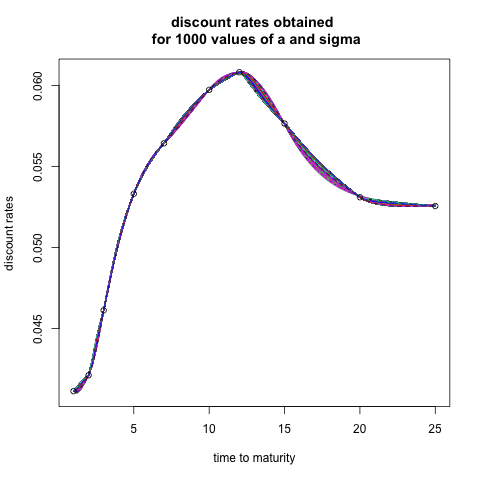
\includegraphics[width=1.065\linewidth, height=0.35\textheight]{gfx/chapter-yc-insurance/construction_graph21}
        \caption{Discount rates obtained for 1000 values of $a \in [0.1, 10]$ and $\sigma \in [0, 0.1]$}
        \label{fig:sensi_a_sigma_1}
    \end{minipage}%
    \begin{minipage}{0.5\textwidth}
        \centering
        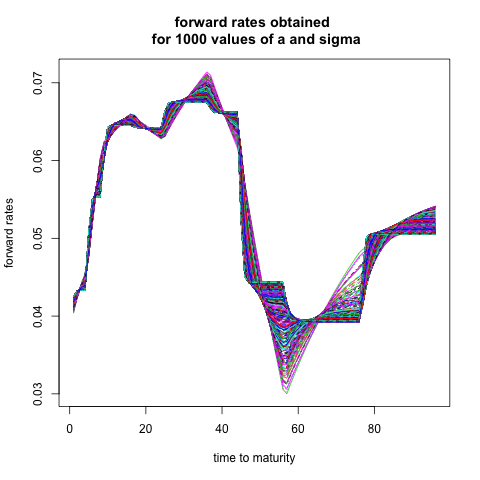
\includegraphics[width=1.065\linewidth, height=0.35\textheight]{gfx/chapter-yc-insurance/construction_graph22}
        \caption{Forward rates obtained for 1000 values of $a \in [0.1, 10]$ and $\sigma \in [0, 0.1]$}
        \label{fig:sensi_a_sigma_2}
    \end{minipage}
  \end{figure}

\subsubsection{Calibration using derivatives}
\label{curvederivatives}

Another way for picking $a$ and $\sigma$ might be to calibrate the underlying short-rate model to a set of caps and swaptions. The optimization procedure would involve the following steps: choosing $a$ and $\sigma$, construct the initial curve with an \textit{exact fit} using the results described in  section \ref{curve_calibration}; use it as an input for theoretical caps and swaptions prices formulas implied by the underlying short-rate model, until $a$ and $\sigma$ which minimize the difference between theoretical and market prices for caps and swaptions are found. 


\subsubsection{Curve extrapolation}
\label{curveextrap}

Using the Hull and White extended Vasicek model, it is possible to derive the instantaneous forward rates from the discount factors formula. We can write:

\begin{equation}
f(0, t) = -\frac{\partial log(P(0,t)}{\partial t} =  X_0e^{-at} + a \int_0^t e^{-a(t-u)}b(u)du-\frac{\sigma^2}{2}\phi^2(t)
\end{equation}

Hence, in our framework, using the fact that $t \mapsto b(t)$ is piecewise constant, we can also write:
\begin{equation}
f^M(0, t) = X_0e^{-at} + a \sum_{i = 1}^n b_i \left[\phi(t-T_{i-1} \wedge t) - \phi(t-T_i \wedge t)\right]+ab_{n+1}\phi(t-T_n \wedge t)-\frac{\sigma^2}{2}\phi^2(t)
\end{equation}
This formula directly provides an input for the simulation of Hull \& White short-rate, with parameters $a$, $\sigma$ and $b_1, \ldots, b_n$ previously calibrated to market data.

\medskip

Hence, let $t$ grow to $\infty$, we have:
\begin{equation}
f^M(0, \infty) = b_{n+1}-\frac{\sigma^2}{2a^2}
\end{equation}

If we assume that the UFR is exogenously chosen, and denote it by $f_\infty$, we are able to derive the parameter $b_{n+1}$ as:

\begin{equation}
b_{n+1} = f_\infty + \frac{\sigma^2}{2a^2}
\end{equation}

This enables to re-write equation (\ref{Intb}), when extrapolation is required, as:

\begin{equation}
\label{Intbbis}
I_{n+1}(t) = \sum_{k=1}^n b_k \left( \xi(t - T_{k-1} \wedge t) -  \xi(t - T_k \wedge t) \right) + \left(f_\infty + \frac{\sigma^2}{2a^2} \right) \xi(t - T_n \wedge t)
\end{equation}

If \textbf{a fixed \textit{ultimate forward rate} (UFR) is defined exogenously}, one can increase or decrease the parameter $a$, to achieve a convergence of $f^M(0, t)$ to $f_\infty$ at a pre-specified maturity. A period of convergence $\tau_{cv}$ after the  \textit{Last Liquid Point} (LLP) is defined. Starting from a low value such as $a = 0.1$, $a$ is increased until:
$$
f^M(0, LLP+\tau_{cv}) = f_\infty
$$
or
$$
|f^M(0, LLP+\tau_{cv}) - f_\infty| < tol
$$
for a given $\sigma$, and a given numerical tolerance $tol$.

\medskip

Otherwise, an \textbf{\textit{ultimate forward rate} (UFR) can be derived from market data}. A static discount curve is fitted to a fraction of the quoted swaps available, called the \textit{training} set. After the construction of the curve on this fraction of the data, we evaluate how well, when extrapolated to a given exogenous UFR, it would price the remaining swaps in a \textit{test} set.

\medskip

The LLP provided by the prudential authority (as of 2016, a maturity 20 years), could be used to define the frontier between the \textit{training} and \textit{test} set. Otherwise,  one can define a percentage of the swaps data to be used as a \textit{training} dataset, for example 80\% or 90\% of the available swaps.

\medskip

Both of these methods for curve extrapolation are applied in the numerical examples, in section \ref{numericalexamples}.

\section{Forecasting with Functional PCA}
\label{curvesforecast}

The idea that a few principal components explain a major part of the changes in bonds returns originates from \cite{litterman1991volatility}. This idea is now well accepted and applied to yield curve forecasting; the interested reader could refer to \cite{diebold2006forecasting} or \cite{christensen2011affine} for example.

\medskip

We use a similar rationale, but apply it somewhat differently. The changes in the swap curve over time, are explained by the changes observed in the calibrated parameters $b_i$s over time. Considering the fact that our model for fitting each cross section of yields is already \textit{overparametrized} (as it uses at least as much parameters as swap rates available in the input dataset), the use of models such as an unrestricted Vector Autoregressive (VAR) to predict the $b_i$s could lead to poor forecasts, with high variance.

\medskip

Functional Principal Components Analysis in the spirit of \cite{ramsay1991some} and \cite{ramsay2005springer}, and more precisely Functional Principal Components Regression, was hence seen as one of the most immediate candidate to achieve a reduction of the problem's dimension. This method is used for example by \cite{hyndman2007robust} for forecasting log mortality rates. It has also been applied in finance, for example in \cite{Benko2007Functional}. 

\medskip

We consider functional data of the form:

\begin{equation}
b^{a, \sigma}_x(t)
\end{equation}

These are the parameters $b_i$s obtained by fitting each cross section of swap rates; observed at increasing times $t \in \left\lbrace t_1, \ldots, t_N \right\rbrace$, for increasing maturities $x \in \left\lbrace x_1, \ldots, x_p \right\rbrace$. The calibration method is the one  described in section \ref{curve_calibration}, with $a$ and $\sigma$ kept fixed over time.

\medskip

\textbf{Finding the Functional Principal Components}

\medskip

Using the approach described in details in \cite{ramsay2005springer}, we let $\textbf{B}$ be the matrix containing at line $i$ and column $j$:
\begin{equation}
\textbf{B}_{i,j} = b^{a, \sigma}_{x_j}(t_i)
\end{equation}

With $i = 1, \ldots, N$ and $j = 1, \ldots, n$, $n > p$. For each cross section of $b_i$s calibrated at time $t_i$, a cubic spline interpolation is applied to $x \mapsto b^{a, \sigma}_{x}(t_i)$, so that the $b_i$s values are now equally spaced on a larger grid of maturities spanning $\left[ x_1, x_p\right]$. Let $w$ be the fixed interpolation step applied to $x \mapsto b^{a, \sigma}_{x}(t_i)$ on $\left[ x_1, x_p\right]$, and:
\begin{equation}
\textbf{V} = \frac{1}{N}\textbf{B}^T\textbf{B}
\end{equation}

$\textbf{V}$ is the covariance matrix of the $b_i$'s, when we consider that the columns of $\textbf{B}$ have been centered. We are then looking for the vectors $\xi^{a, \sigma}$, the (approximate) functional principal components, verifying:
\begin{equation}
w\textbf{V}\xi^{a, \sigma} = \rho \xi^{a, \sigma}
\end{equation}

This is equivalent to searching the eigenvalues and eigenvectors of $\textbf{V}$, so that:
\begin{equation}
\textbf{V} u = \lambda u
\end{equation}
and $\rho = w \lambda$. This problem of finding eigenvalues and eigenvectors of $\textbf{V}$ is typically solved by using the Singular Value Decomposition (SVD) of \textbf{B}, and taking the normalized right singular vectors as functional principal components. The interested reader can refer to \cite{jolliffe2002principal} and \cite{ramsay2005springer} for details. Another interesting resource on Functional Principal Component Analysis is \cite{shang2014survey}.

\medskip

\textbf{Forecasting using Principal Components regression}

\medskip

Having obtained the functional principal components, a least squares regression of the cross sections of $b_i$s is carried out. The $b_i$s are expressed as a linear combination of the previously constructed functional principal components, plus an error term:
\begin{equation}
\forall t \in \left\lbrace t_1, \ldots, t_N \right\rbrace, \: b^{a, \sigma}_{x}(t) = \beta_{t, 0} + \sum_{k = 1}^K \beta_{t, k} \xi^{a, \sigma}_k(x) + \epsilon_t(x)
\end{equation}

$K$ is the number of functional principal components. These functional principal components are not highly correlated by construction, so that we can use univariate time series forecasts for each of the $K+1$ time series, and h-step ahead forecasts of the $b_i$s as:

\begin{equation}
\hat{b}^{a, \sigma}_{x}(t+h) = \hat{\beta}_{t+h|t, 0} + \sum_{k = 1}^K \hat{\beta}_{t+h|t, k} \xi^{a, \sigma}_k(x)
\end{equation}

\medskip

Once the forecasts $\hat{b}^{a, \sigma}_{x}(t+h)$ are obtained, they can be plugged into formulae from section \ref{calibr_bi} to deduce h-step ahead forecasts for the discount factors and discount rates.

\medskip

For choosing \textit{good} values for $a$, $\sigma$ and $K$, we typically used a cross-validation on grids of values for these three parameters, and rolling origin estimation/forecasting, as described in section \ref{numericalexamples}.

\section{Numerical examples}
\label{numericalexamples}

In order to illustrate how the methods described in the previous sections work, we use IRS and OIS data from \cite{andersen2007discount}, \cite{andersen2010interest}, \cite{ametrano2013everything}, an example of bonds data from \cite{hagan2006interpolation}; \textit{a curve where all cubic splines produce negative forward rates}. For forecasting the curves, we use market EUR 6M IRS data, (from which we give detailed summaries) with a CRA adjustment equal to $10$bps.

\medskip

For the data from \cite{andersen2010interest}, we assume that the swaps cash-flows payments occur on an annual basis as for OIS. From \cite{ametrano2013everything}, we consider mid quotes from Eonia OIS and 6-month Euribor IRS as of December 11, 2012. These data sets are all reproduced in the appendices.

\medskip

In section \ref{andersen2010examples}, four calibration methods are tested to illustrate section \ref{curve_calibration}. The method proposed in this paper \footnote{Actually applied to Hull \& White model, but which can be applied to other short-rate models.} is denoted by CMN. It is compared to two iterative curve calibration methods, with linear (LIN) and natural cubic splines (SPL) interpolation on missing dates, and the \cite{smithwilson2001} method (SW). Section \ref{andersen2007examples} also illustrates \ref{curve_calibration}. We use a dataset from \cite{andersen2007discount}; a direct \textit{bootstrapping} without regularization produces wiggly spot and forward rates. The effects of the regularization of approximate second derivative for forward rates and calibrated $b_i$'s is illustrated. Such a regularization could also be applied to noisy bonds data.

\medskip

In section \ref{curvehagan}, the interpolation method is tested on a \textit{curve where all cubic methods produce negative forward rates}, from \cite{hagan2006interpolation}. Section \ref{curveextrapexamples} illustrates the possible extrapolation methods described in  section \ref{curveextrap}. \ref{forecastexample} illustrates the curves' forecasting method introduced in section \ref{curvesforecast}.

\medskip

The discount factors usually display no particular subtleties, so they are deliberately omitted. We present discount rates and discrete forwards instead, and the discrete forwards are taken to be 3-month forward rates.

\subsection{Curve calibration}

\subsubsection{On swaps data from \cite{andersen2010interest}}
\label{andersen2010examples}

Below on figures \ref{fig:andersen2010examples1}, \ref{fig:andersen2010examples2}, \ref{fig:andersen2010examples3}, \ref{fig:andersen2010examples4},  are the discount rates and discrete forwards obtained for the four methods described in the previous section; two \textit{bootstrapping} methods, with linear (LIN) and natural cubic splines (SPL) interpolation on missing dates, the \cite{smithwilson2001} method (SW), and the method described in \ref{curve_calibration} with an exact fit, denoted as CMN. The discount rates are presented as a dashed line, and the forward rates as a plain colored line.


\medskip
\begin{figure}[!htb]
    \centering
    \begin{minipage}{.5\textwidth}
        \centering
        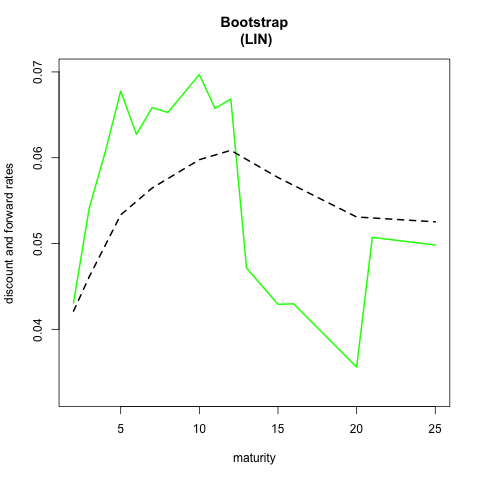
\includegraphics[width=1.06\linewidth, height=0.37\textheight]{gfx/chapter-yc-insurance/construction_graph1}
        \caption{\textit{Bootstrapping} with linear interpolation}
        \label{fig:andersen2010examples1}
    \end{minipage}%
    \begin{minipage}{0.5\textwidth}
        \centering
        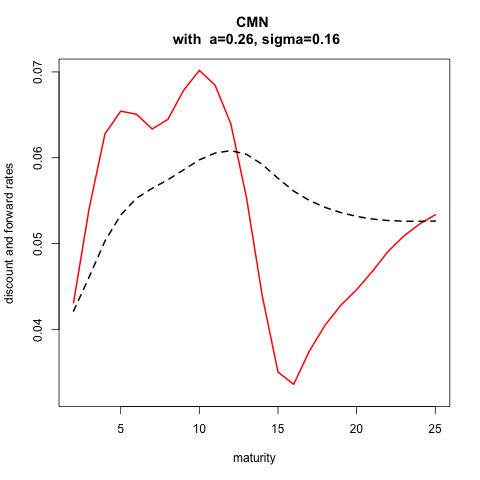
\includegraphics[width=1.06\linewidth, height=0.37\textheight]{gfx/chapter-yc-insurance/construction_graph2}
        \caption{CMN applied to Hull and White extended Vasicek}
        \label{fig:andersen2010examples2}
    \end{minipage}
  \end{figure}

  \begin{figure}[!htb]
        \begin{minipage}{0.5\textwidth}
        \centering
        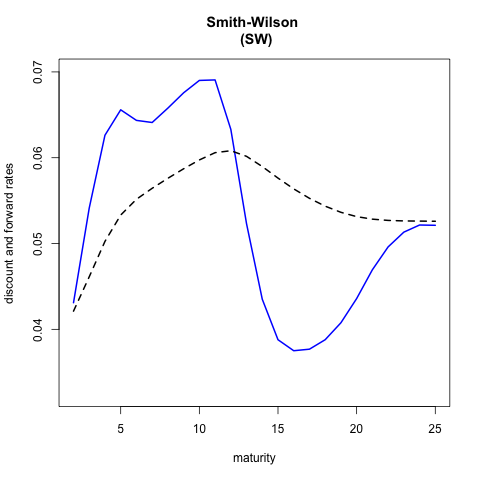
\includegraphics[width=1.06\linewidth, height=0.37\textheight]{gfx/chapter-yc-insurance/construction_graph3}
        \caption{Smith-Wilson method}
        \label{fig:andersen2010examples3}
    \end{minipage}
        \begin{minipage}{0.5\textwidth}
        \centering
        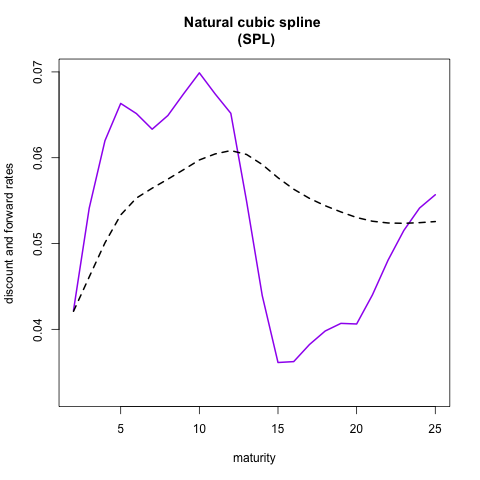
\includegraphics[width=1.06\linewidth, height=0.37\textheight]{gfx/chapter-yc-insurance/construction_graph4}
        \caption{Natural cubic spline}
        \label{fig:andersen2010examples4}
    \end{minipage}
\end{figure}

As demonstrated on figures \ref{fig:andersen2010examples1}, \ref{fig:andersen2010examples2}, \ref{fig:andersen2010examples3} and \ref{fig:andersen2010examples4}, the discount rates produced by the four methods are quite similar. The discrete forward rates better exhibit the differences between them. 

\medskip

Curve construction with linear interpolation between quoted swaps maturities (on figure \ref{fig:andersen2010examples1}), produces a saw-tooth like forward curve, which might not be desirable, and the other methods produce more regular forward curves.

\medskip

For the method described in this paper - denoted as CMN on figure \ref{fig:andersen2010examples2} - and applied to the extended Vasicek model, the discrete forwards (with an exact fit required, as described in section ~\ref{curve_calibration}) reflect the fact that the discount factors' construction relies on a piece-wise constant function, with slight changes in first derivatives at quoted swap maturities. This effect remains very reasonable however, as the discrete forward curve is highly similar to those produced by the other models, and doesn't exhibit large changes at quoted swap maturities.

\medskip

With $a$=\code{0.2557}, $\sigma$=\code{0.1636}, the parameters $b_i$s from table \ref{tab:andersen2010tables1} are obtained. They are presented along with the parameters $\xi_i$s obtained by the method in \cite{smithwilson2001}, with $a = 0.1$. $a = 0.1$ is actually given as default parameter by Solvency II's  technical specifications, and using the notations from QIS5 technical specifications.


\begin{table}[!htb]
\begin{center}
% table caption is above the table
\caption{Parameters obtained for CMN and Smith-Wilson}
\label{tab:andersen2010tables1}       % Give a unique label
% For LaTeX tables use
\begin{tabular}{llllllllll}
\hline\noalign{\smallskip}
Maturity & $b_i$ & $\xi_i$  \\
\noalign{\smallskip}\hline\noalign{\smallskip}
  1 & 0.0661  & -16.680\\
  2 & 0.1894  & 23.556\\
  3 & 0.2523  & -0.8413\\
  5 & 0.2523  & -8.9116\\
  7 & 0.2523  & 3.3552\\
  10 & 0.2806 & 7.9600\\
  12 & 0.2523 & -14.098\\
  15 & 0.2089 & 3.9119\\
  20 & 0.2553 & 3.4828\\
  25 & 0.2616 & -1.9497\\
\noalign{\smallskip}\hline
\end{tabular}
\end{center}
\end{table}

\subsubsection{On noisy swaps data}
\label{andersen2007examples}

This section illustrates what may happen if the method from section ~\ref{curve_calibration} is applied directly to noisy data, without regularization of the parameters. We use data from \cite{andersen2007discount}.

\medskip

Figure \ref{fig:andersen2007examples1} on the left describes the discount and forward rates obtained without regularization, with $a = 0.3655$ and $\sigma =  0.0037$. On the right, figure \ref{fig:andersen2007examples2} describes the discount and forward rates obtained  by minimizing the objective function in equation (\ref{problem3}), and using the parameters $\lambda_1 = 1e-08$ and $\lambda_2 = 1e-05$, $a = 9.8891$ and $\sigma =  0.3957$.

  \begin{figure}[!htb]
    \centering
    \begin{minipage}{.5\textwidth}
        \centering
        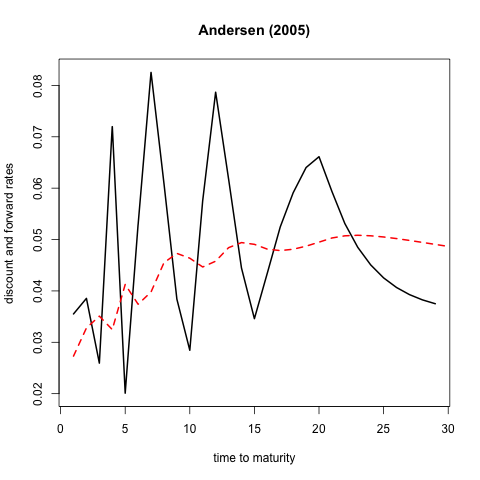
\includegraphics[width=1.05\linewidth, height=0.35\textheight]{gfx/chapter-yc-insurance/construction_graph7}
        \caption{Curve calibration without regularization}
        \label{fig:andersen2007examples1}
    \end{minipage}%
    \begin{minipage}{0.5\textwidth}
        \centering
        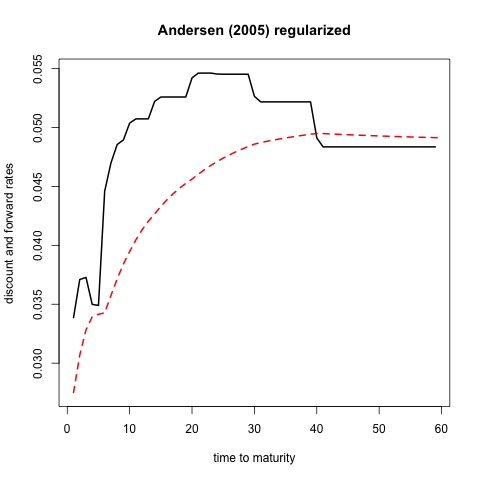
\includegraphics[width=1.05\linewidth, height=0.35\textheight]{gfx/chapter-yc-insurance/construction_graph8}
        \caption{Curve calibration with regularization}
        \label{fig:andersen2007examples2}
    \end{minipage}
  \end{figure}
  
In order to pick $\lambda_1$ and $\lambda_2$, we make a grid search on couples $(\lambda_1, \lambda_2)$. For each $(\lambda_1, \lambda_2)$, a minimization based on derivatives is applied, with multiple restarts of the minimization algorithm. Multiple restarts avoid getting trapped into local minima.

\medskip

Table \ref{tab:andersen2007tables1} contains both the unregularized and regularized $b_i$s. The unregularized ones naturally exhibit a higher variance, because an exact fit to each swap rate in the noisy dataset is required. The regularized $b_i$s exhibit a lower variance, at the expense of a higher bias in the fitting of the data from \cite{andersen2007discount}.

\begin{table}
\begin{center}
% table caption is above the table
\caption{Parameters obtained for unregularized and regularized CMN}
\label{tab:andersen2007tables1}       % Give a unique label
% For LaTeX tables use
\begin{tabular}{llllllllll}
\hline\noalign{\smallskip}
Maturity & unregularized $b_i$ & regularized $b_i$  \\
\noalign{\smallskip}\hline\noalign{\smallskip}
  0.5 & 0.0253  & 0.0281\\
  1 & 0.1100  & 0.0363\\
  1.5 & -0.0078  & 0.0383\\
  2 & 0.0929  & 0.0383\\
  2.5 & -0.0005  & 0.0380\\
  3 & -0.1360  & 0.0352\\
  4 & 0.2901  & 0.0358\\
  5 & 0.1975  & 0.0478\\
  7 & 0.1654  & 0.0497\\
  10 & -0.0056 & 0.0515\\
  12 & 0.1315 & 0.0533\\
  15 & 0.1392 & 0.0554\\
  20 & 0.0688 & 0.0553\\
  30 & 0.039 & 0.0491\\
\noalign{\smallskip}\hline
\end{tabular}
\end{center}
\end{table}

\subsubsection{On \textit{a curve where all cubic methods produce negative forward rates}, with data from \cite{hagan2006interpolation}}
\label{curvehagan}

The dataset from this section is used in \cite{hagan2006interpolation}, and is described as \textit{a curve where all cubic methods produce negative forward rates}. It is reproduced in the appendices.

\medskip

Figure \ref{fig:hagan2006examples1} illustrates the discount rates (dashed line), and discrete forward rates (plain coloured line) obtained with a linear interpolation of the bond yields. The discrete forward remain positive on all maturities, but again exhibit a sawtooth profile. As expected, the natural cubic spline on figure \ref{fig:hagan2006examples2} produces negative discrete forward rates on this dataset.

\begin{figure}[!htb]
    \centering
    \begin{minipage}{.5\textwidth}
        \centering
        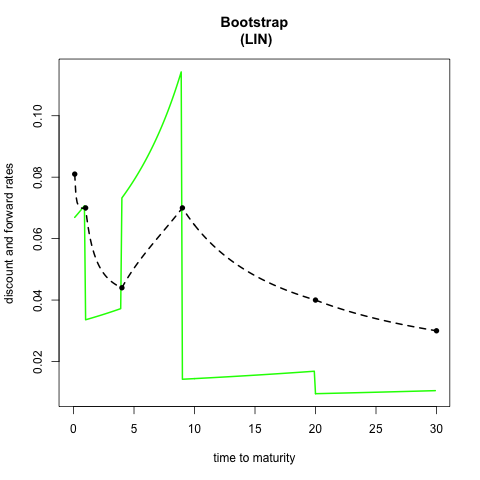
\includegraphics[width=1.06\linewidth, height=0.285\textheight]{gfx/chapter-yc-insurance/construction_graph13}
        \caption{Linear interpolation on \textit{a curve where all cubic methods produce negative forward rates}}
        \label{fig:hagan2006examples1}
    \end{minipage}%
    \begin{minipage}{0.5\textwidth}
        \centering
        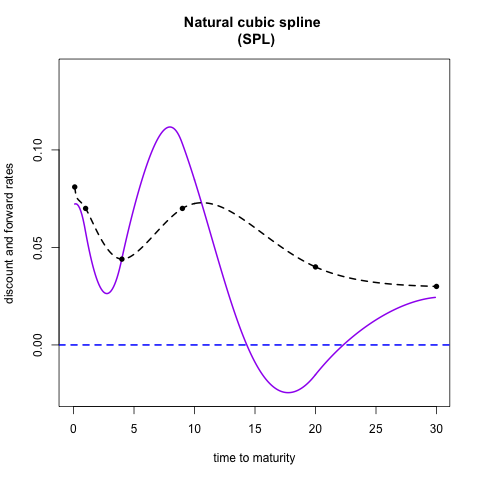
\includegraphics[width=1.06\linewidth, height=0.285\textheight]{gfx/chapter-yc-insurance/construction_graph16}
        \caption{Natural cubic spline interpolation on \textit{a curve where all cubic methods produce negative forward rates}}
        \label{fig:hagan2006examples2}
    \end{minipage}
  \end{figure}
  
  
\begin{figure}[!htb]
    \centering
    \begin{minipage}{.5\textwidth}
        \centering
        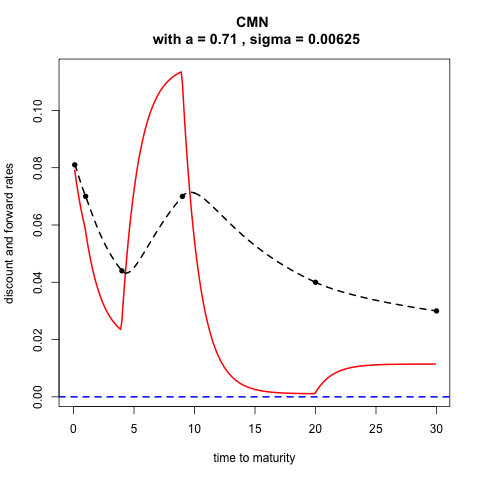
\includegraphics[width=1.06\linewidth, height=0.35\textheight]{gfx/chapter-yc-insurance/construction_graph14}
        \caption{CMN interpolation on \textit{a curve where all cubic methods produce negative forward rates}}
        \label{fig:hagan2006examples3}
    \end{minipage}%
    \begin{minipage}{0.5\textwidth}
        \centering
        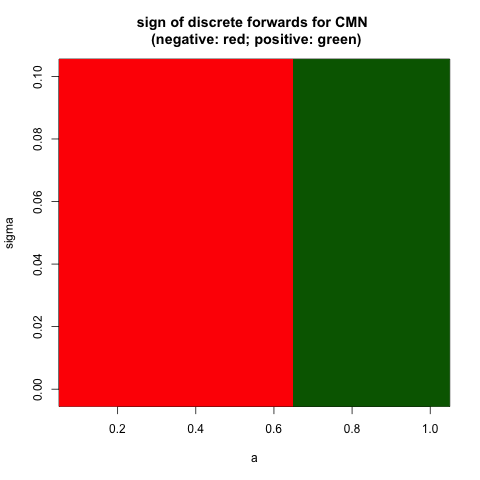
\includegraphics[width=1.06\linewidth, height=0.35\textheight]{gfx/chapter-yc-insurance/construction_graph17}
        \caption{Sign of discrete forwards for CMN as function of $a$ and $\sigma$, on \textit{a curve where all cubic methods produce negative forward rates}}
        \label{fig:hagan2006examples4}
    \end{minipage}
  \end{figure}
  
Figures \ref{fig:hagan2006examples3} and \ref{fig:hagan2006examples4} present the results obtained on data from \cite{hagan2006interpolation}. Figure \ref{fig:hagan2006examples4} presents the sign of discrete forward rates as a function of $a$ and $\sigma$. We consider that discrete forward rates' sign is negative if a least one discrete forward rate is negative. We observe on both figures \ref{fig:hagan2006examples3} and \ref{fig:hagan2006examples4} that a low value of $a$ might produce negative forward rates on maturities comprised between $15$ and $20$. But a high value always produces positive forward rates.

\medskip

This is explained by what we saw in section \ref{curveextrap}: in the Hull and White extend Vasicek case, $a$ controls the speed of convergence of forward rates to the UFR: the higher the $a$, the faster the convergence of forward rates to the UFR on long-term maturities. The parameters obtained by CMN interpolation (for producing figure \ref{fig:hagan2006examples3}), with $a = 0.71$ and $\sigma = 0.0062$ are presented in table \ref{tab:hagan2006tables1}.

\begin{table}[!htb]
\begin{center}
% table caption is above the table
\caption{Parameters obtained CMN with $a = 0.71$ and $\sigma = 0.0062$ on \cite{hagan2006interpolation} data}
\label{tab:hagan2006tables1}       % Give a unique label
% For LaTeX tables use
\begin{tabular}{llllll}
\hline\noalign{\smallskip}
Maturity & $b_i$  \\
\noalign{\smallskip}\hline\noalign{\smallskip}
  0.1 & 0.0718\\
  1 & 0.0351  \\
  4 & 0.0018 \\
  9 & 0.1162  \\
  20 & 0.0011\\
  30 & 0.0114\\
\noalign{\smallskip}\hline
\end{tabular}
\end{center}
\end{table}

\subsection{Curve extrapolation on data from \cite{ametrano2013everything}}
\label{curveextrapexamples}

In this section, we use the extrapolation methods described in \ref{curveextrap}, on OIS and IRS (with CRA adjustment equal to $10$bps) data from \cite{ametrano2013everything}.

\subsubsection{With Solvency II technical specifications, on IRS + CRA}

Extrapolation to a fixed UFR equal to $4.2\%$ is tested, using CMN and the Smith-Wilson method. For both methods, the Last Liquid Point (LLP) is equal to 20 years, and convergence to the UFR is forced to 40 years after the LLP.

\medskip

For the CMN method, the parameters are $a = 0.174$ and $\sigma = 0.0026$, and for the Smith-Wilson method,  $a = 0.125$. The resulting discount and forward curves are presented in figures \ref{fig:extrapCMNSII1} and \ref{fig:extrapSWSII1}, and the parameters $b_i$s and $\xi_i$s in table \ref{tab:ametrano2013tables1}.

\begin{figure}[!htb]
    \centering
    \begin{minipage}{.5\textwidth}
        \centering
        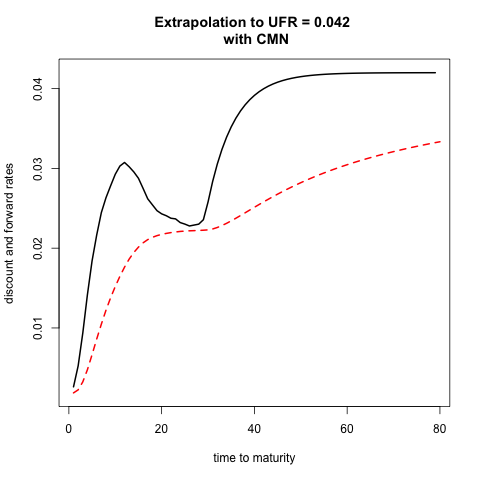
\includegraphics[width=1.065\linewidth, height=0.4\textheight]{gfx/chapter-yc-insurance/construction_graph18}
        \caption{Extrapolation to $UFR = 4.2\%$ with CMN}
        \label{fig:extrapCMNSII1}
    \end{minipage}%
    \begin{minipage}{0.5\textwidth}
        \centering
        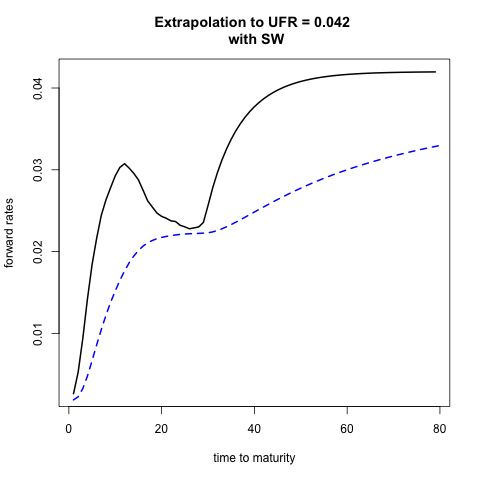
\includegraphics[width=1.065\linewidth, height=0.4\textheight]{gfx/chapter-yc-insurance/construction_graph19}
        \caption{Extrapolation to $UFR = 4.2\%$ with Smith-Wilson}
        \label{fig:extrapSWSII1}
    \end{minipage}
  \end{figure}

\begin{table}
\begin{center}
% table caption is above the table
\caption{Parameters for CMN ($b_i$) and Smith-Wilson ($\xi_i$) extrapolation}
\label{tab:ametrano2013tables1}       % Give a unique label
% For LaTeX tables use
\begin{tabular}{llllllllllllllllllllllllllllll}
\hline\noalign{\smallskip}
Maturity & $b_i$ & $\xi_i$  \\
\noalign{\smallskip}\hline\noalign{\smallskip}
  1 & 0.0019  & -2.5888\\
  2 & 0.0112  & 0.7585\\
  3 & 0.0266  & 0.1415\\
  4 & 0.0352  & 1.3153\\
  5 & 0.0438  & 0.4726\\
  6 & 0.0378  & -0.8809\\
  7 & 0.0399  & 1.2010\\
  8 & 0.0387  & -0.8965\\
  9 & 0.0338  & -0.3536\\
  10 & 0.0376 & 0.7268\\
  11 & 0.0363 & -0.1582\\
  12 & 0.0353 & 1.2852\\
  13 & 0.0312 & -1.9866\\
  14 & 0.0239 & 0.4161\\
  15 & 0.0285 & 0.7056\\
  16 & 0.0211 & -0.7112\\
  17 & 0.0208 & -1.7105\\
  18 & 0.0182 & 1.9922\\
  19 & 0.0248 & -1.5542\\
  20 & 0.0172 & 0.5125\\
  21 & 0.0272 & 1.0148\\
  22 & 0.0189 & -2.1158\\
  23 & 0.0025 & 3.4051\\
  24 & 0.0021 & -3.7822\\
  25 & 0.0020 & 2.7013\\
  26 & 0.0239 & -2.8668\\
  27 & 0.0195 & 2.2513\\
  28 & 0.0274 & -0.8877\\
  29 & 0.0202 & -7.1463\\
  30 & 0.0326 & 8.5322\\
\noalign{\smallskip}\hline
\end{tabular}
\end{center}
\end{table}

\medskip

The discount and forward curves produced by both methods are similar, as seen on figures \ref{fig:extrapCMNSII1} and \ref{fig:extrapSWSII1}. The convergence of the Smith-Wilson method to the UFR seems to be slighty faster. This is caused by the fact that for CMN, we use instantaneous forward rates to assess the convergence to the UFR, whereas for the Smith-Wilson method, we use discrete forwards.

\subsubsection{With OIS data, and a data driven UFR}

For this example, we use OIS data from \cite{ametrano2013everything} presented in the appendices. A training set containing 14 swap rates ($90\%$ of the dataset) with increasing maturities starting at $1$ and ending at $20$ is made up. 

\medskip

This training set is used to construct the discount curve, which is then extrapolated to $30$-year maturity and beyond, using different values for the UFR. The two remaining swaps, with maturities equal to $25$ and $30$, are placed into the test set.

\begin{figure}[!htb]
    \centering
    \begin{minipage}{.5\textwidth}
        \centering
        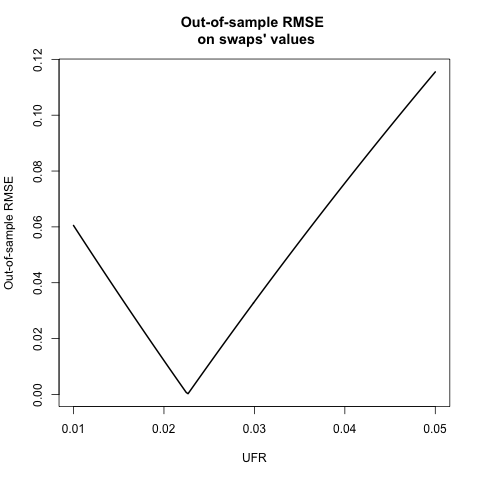
\includegraphics[width=1.06\linewidth, height=0.35\textheight]{gfx/chapter-yc-insurance/construction_graph20_1}
        \caption{Out-of-sample RMSE on swap values, as a function of UFR}
        \label{fig:datadrivenUFR1}
    \end{minipage}%
    \begin{minipage}{0.5\textwidth}
        \centering
        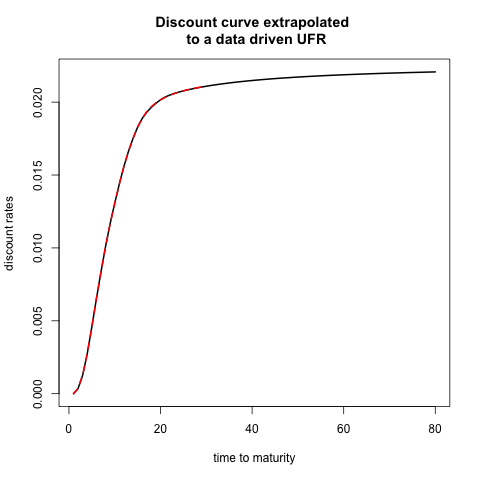
\includegraphics[width=1.06\linewidth, height=0.35\textheight]{gfx/chapter-yc-insurance/construction_graph20_2}
        \caption{Extrapolation of OIS curve to a data driven $UFR = 0.0226$}
        \label{fig:datadrivenUFR2}
    \end{minipage}
  \end{figure}
  
Figure \ref{fig:datadrivenUFR1} presents the out-of-sample RMSE obtained on swaps values from the  test set, as a function of UFR. This error decreases until $UFR = 0.0226$ (notice that this value would depend on the step chosen on the grid of UFRs), and then, starts to increase again. Figure \ref{fig:datadrivenUFR2} displays the discount curve constructed on the training set, extrapolated to a 80-year maturity with an UFR equal to $0.0226$ (the one minimizing the out-of-sample RMSE on the chosen grid of UFRs) is presented.

\subsection{12-months ahead forecast on historical IRS + CRA}
\label{forecastexample}

In this section, we apply ideas from section \ref{curvesforecast} to real world IRS data observed monthly from december 2013 to april 2016, adjusted from a CRA equal to $10$bps.

\medskip

Figure \ref{fig:forecast1} and table \ref{tab:realdatatables1} are to be read together. They  contain the informations on the spot rates derived from the IRS data adjusted from a CRA, using CMN with $a = 0.3655$ and $\sigma = 0.0037$ (other values than $a = 0.3655$ and $\sigma = 0.0037$ would produce the same results as the fitting is exact for many different values of these parameters).

\medskip

The static curves are generally upward sloping, and as time passes, lower and lower spot rates are encountered. In addition, negative rates are observed in table \ref{tab:realdatatables1}; which is coherent with the current context.

\begin{figure}[!htb]
\centering
% Use the relevant command to insert your figure file.
% For example, with the graphicx package use
  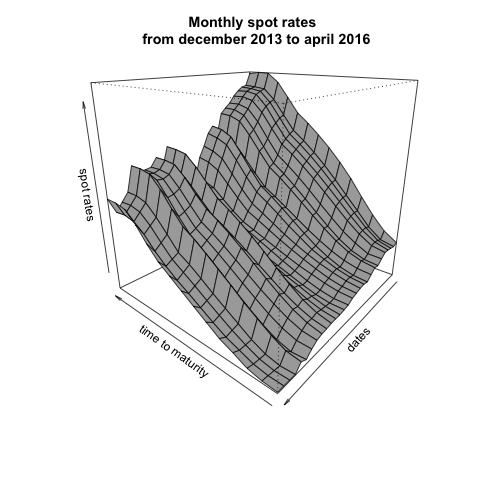
\includegraphics[width=0.75\textwidth]{gfx/chapter-yc-insurance/forecasting_graph1}
% figure caption is below the figure
\caption{Spot rates observed from december 2013 to april 2016}
\label{fig:forecast1}       % Give a unique label
\end{figure}

\begin{table}
\begin{center}
% table caption is above the table
\caption{Descriptive statistics for the spot rates observed from december 2013 to april 2016}
\label{tab:realdatatables1}       % Give a unique label
% For LaTeX tables use
\begin{tabular}{lllllll}
\hline\noalign{\smallskip}
Maturity & Min. & 1st Qrt & Median & Mean & 3rd Qrt & Max.\\
\noalign{\smallskip}\hline\noalign{\smallskip}
  1  & -0.0026 & -0.0008 & 0.0000 & 0.0003  & 0.0019  & 0.0031\\
  3  & -0.0023 & 0.0002  & 0.0009 & 0.0013  & 0.0028  & 0.0065\\
  5  & -0.0008 & 0.0017  & 0.0030 & 0.0037  & 0.0056  & 0.0117\\
  10 & 0.0046  & 0.0059  & 0.0090 & 0.0101  & 0.0132  & 0.0211\\
  15 & 0.0063  & 0.0097  & 0.0127 & 0.0141  & 0.0179  & 0.0258\\
  20 & 0.0069  & 0.0113  & 0.0144 & 0.0157  & 0.0199  & 0.0272\\
  30 & 0.0071  & 0.0118  & 0.0155 & 0.0164  & 0.0208  & 0.0270\\
\noalign{\smallskip}\hline
\end{tabular}
\end{center}
\end{table}

\subsubsection{Benchmarking the model}
\label{benchmarking}

\begin{table}
\begin{center}
% table caption is above the table
\caption{Average out-of-sample error on real world IRS data + CRA}
\label{tab:benchmarktables1}       % Give a unique label
% For LaTeX tables use
\begin{tabular}{llllll}
\hline\noalign{\smallskip}
Method & Parameters  & Avg. OOS error  \\
\noalign{\smallskip}\hline\noalign{\smallskip}
  CMN - \code{auto.arima} & $K = 5$, $a = 1$, $\sigma = 0.1555$ & 0.0031\\
  CMN - \code{ets} & $K = 5$, $a = 1$, $\sigma = 0.2$ & 0.0037 \\
\hline\noalign{\smallskip}
  NS - \code{auto.arima} & $\lambda = 1.8889$ & 0.0031\\
  NS - \code{ets} & $\lambda = 1.8889$ & 0.0035 \\
\hline\noalign{\smallskip}
  NSS - \code{auto.arima} & $\lambda_1 = 21$, $\lambda_2 = 21$ & 0.0027\\
  NSS - \code{ets} & $\lambda_1 = 7$, $\lambda_2 = 3$ & 0.0035 \\
\noalign{\smallskip}\hline
\end{tabular}
\end{center}
\end{table}

Benchmarks are subjective. The one presented in this section does not aim at showing that one method is always superior to the other. It aims at showing that the method presented in this paper produces forecasts which are (more than) reasonable, and actually close to other well-known methods forecasts (on this given dataset).

\medskip

Forecasts from the model presented in section \ref{curvesforecast} are hence compared to those of two other models constructed in the spirit of by the \cite{diebold2006forecasting}. The cross sections of yields described by figure \ref{fig:forecast1} and table \ref{tab:realdatatables1} are fitted by the \cite{nelson1987parsimonious} model (NS), and its extension by \cite{svensson1994estimating} (NSS). The formulas for the spot rates from these models are respectively:

\begin{equation}
\label{NSyield}
R^M(t, T) = \beta_{t, 1} + \beta_{t, 2} \left[ \frac{1 - e^{-T/\lambda}}{T/\lambda}\right] + \beta_{t, 3} \left[ \frac{1 - e^{-T/\lambda}}{T/\lambda} - e^{-T/\lambda} \right]
\end{equation}

and

\begin{eqnarray}
R^M(t, T) &=& \beta_{t, 1} + \beta_{t, 2} \left[ \frac{1 - e^{-T/\lambda_1}}{T/\lambda_1}\right] + \beta_{t, 3} \left[ \frac{1 - e^{-T/\lambda_1}}{T/\lambda_1} - e^{-T/\lambda_1} \right] \\
&+&\beta_{t, 4} \left[ \frac{1 - e^{-T/\lambda_2}}{T/\lambda_2} - e^{-T/\lambda_2} \right]
\end{eqnarray}

Forecasts $\hat{R}^M(t+h, T)$ are obtained by fitting univariate time series to the parameters $\beta_{t, i}, i = 1, \ldots, 4$ with automatic ARIMA (\code{auto.arima}) and exponential smoothing (\code{ets}) models from \cite{hyndman2008automatic}. This automatic selection is done only for the sake of the benchmarking exercise, and in order to conduct the experience in fairly similar conditions for all the methods. In practice, a visual inspection and an actual study of the univariate time series would of course be required.

\medskip

For all the methods the six methods, CMN, NS, NSS with \code{auto.arima} and \code{ets}, we obtain 12-months ahead forecasts, from rolling estimation windows of a fixed 6 months length, starting in december 2013. That is, the models are trained on 6 months data, and predictions are made on 12 months data; successively. The average out-of-sample RMSE are then calculated for each method, on the whole surface of observed and forecasted yields.

\medskip

The \textit{best} parameters for CMN are obtained by cross-validation, with $K \in \left\lbrace 2, 3, 4, 5, 6\right\rbrace$, $5$ values of $a$ comprised between $0.9$ and $1$, and $10$ values of $\sigma$ comprised between $0$ and $0.2$. For NS and NSS, $\lambda_1$ and $\lambda_2$ are chosen by cross-validation, using the rolling estimation/forecasting we have just described.
\subsubsection{Bootstrap simulation of 12-months ahead spot rates}

In this section, we use the last 12 months of the dataset to construct the functional principal components. Using 12 months as the length of the fixed window for estimation, we get an average out-of-sample RMSE of $0.0026$ (on a smaller number of testing samples than the 6 months estimation window, of course).

\medskip

An AR(1) is fitted to the observed univariate time series $(\beta_{t, i})_t$, $i = 0, \ldots, K$, with $a = 1$, $\sigma = 0.0089$, and $K = 3$ chosen by cross-validation. The three functional principal components' characteristics are summarized in table \ref{tab:boot1}. We notice that the first functional principal component explains already $99.2415\%$ of the changes in $b_i$s, and the first three functional principal components selected by cross-validation explain $99.9220\%$.

\begin{table}
\begin{center}
% table caption is above the table
\caption{Importance of Principal components}
\label{tab:boot1}       % Give a unique label
% For LaTeX tables use
\begin{tabular}{llll}
\hline\noalign{\smallskip}
Indicator & PC1 & PC2 & PC3 \\
\noalign{\smallskip}\hline\noalign{\smallskip}
  Standard deviation & 0.1286 & 0.2461 & 0.2246\\
  Proportion of variance (in $\%$) & 99.2415 & 0.5489 & 0.1315\\
  Cumulative Proportion (in $\%$) & 99.2415 & 99.7904 & 99.9220\\
\noalign{\smallskip}\hline
\end{tabular}
\end{center}
\end{table}

% \begin{figure*}[!htb]
% \centering
% % Use the relevant command to insert your figure file.
% % For example, with the graphicx package use
%   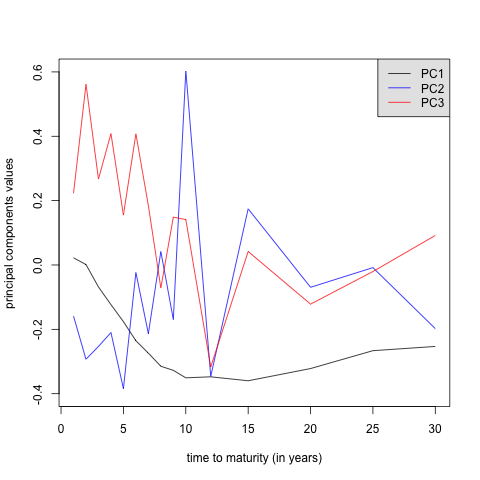
\includegraphics[width=0.6\textwidth]{forecasting_graph5}
% % figure caption is below the figure
% \caption{Principal components of the $b_i$s from april 2015 to april 2016}
% \label{fig:forecast2}       % Give a unique label
% \end{figure*}

\medskip

Figure \ref{forecast:3} presents the autocorrelation functions of the residuals of AR(1)  fitted to $(\beta_{t, i}),  \: i = 0, \ldots, 3$ from april 2015 to april 2016. The residuals from AR(1) fitted to $(\beta_{t, i})_t, \: i = 1, \ldots, 3$ could be considered as stationary, but those from the AR(1) fitted to $(\beta_{t, 0})_t$ seems to be closer to an AR(4).

\medskip

We denote these residuals by $(\epsilon_{t, i})_t, \: i = 0, \ldots, 3$. In order to obtain simulations for the $(\beta_{t, i})_t,  \: i = 0, \ldots, 3$, it is possible to use a Gaussian hypothesis on the residuals. We choose to create one thousand bootstrap resamples with replacement of the $(\epsilon_{t, i})_t, \: i = 0, \ldots, 3$ \footnote{Even if for $\epsilon_{t, 0}$, considering figure \ref{forecast:3}, this makes a strong stationarity assumption on the residuals.}, denoted as $(\epsilon_{t, i}^*)_t, \: i = 0, \ldots, 3$, and create new pseudo values for $(\beta_{t, i}),  \: i = 0, \ldots, 3$:
$$
\beta^*_{t, i} = \beta_{t, i} + \epsilon_{t, i}^*,  \: i = 0, \ldots, 3
$$

\medskip

Having done this, AR(1) forecasts $\beta^*_{t+h|t, i}$ can be obtained, in order to construct:

\begin{equation}
\hat{b}^{a, \sigma, *}_{x}(t+h) = \hat{\beta}^*_{t+h|t, 0} + \sum_{k = 1}^K \hat{\beta}^*_{t+h|t, k} \xi^{a, \sigma}_k(x)
\end{equation}

\medskip

The $\hat{b}^{a, \sigma, *}_{x}(t+h)$ can then be plugged into formulae \ref{la_formule} and \ref{Intb} to deduce simulations of h-step ahead forecasts for the discount factors and discount rates.

\medskip

The simulations (1000) of 12-months ahead discount rates are presented in figures \ref{forecast:4} and \ref{forecast:5}.

\begin{figure}[!htb]
\centering
% Use the relevant command to insert your figure file.
% For example, with the graphicx package use
  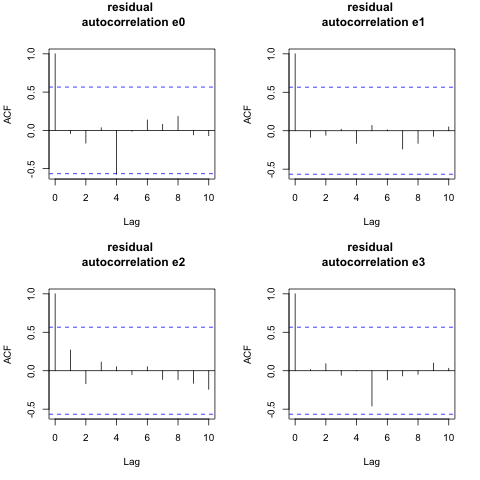
\includegraphics[width=0.85\textwidth]{gfx/chapter-yc-insurance/forecasting_graph2}
% figure caption is below the figure
\caption{Autocorrelation functions for the residuals of univariate time series(AR(1)) on $\beta_0$, $\beta_1$, $\beta_2$, $\beta_3$}
\label{forecast:3}       % Give a unique label
\end{figure}

\begin{figure}[!htb]
    \centering
    \begin{minipage}{.5\textwidth}
        \centering
        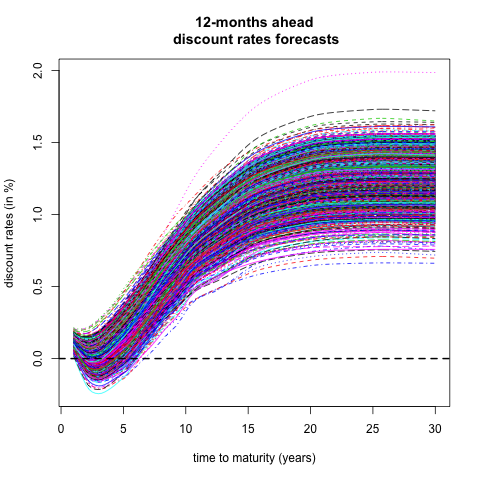
\includegraphics[width=0.8\linewidth, height=0.3\textheight]{gfx/chapter-yc-insurance/forecasting_graph3}
        \caption{Curves simulated with principal components from april 2015 to april 2016, and bootstrap ressampling of the residuals}
        \label{forecast:4}
    \end{minipage}%
    \begin{minipage}{0.5\textwidth}
        \centering
        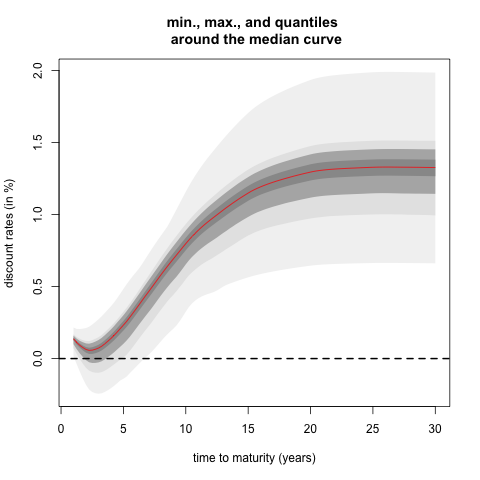
\includegraphics[width=0.8\linewidth, height=0.3\textheight]{gfx/chapter-yc-insurance/forecasting_graph4}
        \caption{Min., Max., and quartiles around the median curve for the simulations}
        \label{forecast:5}
    \end{minipage}
  \end{figure}

\begin{table}
\begin{center}
% table caption is above the table
\caption{Descriptive statistics for fitted parameters $b_i$s from april 2015 to april 2016}
\label{tab:realdatatables2}       % Give a unique label
% For LaTeX tables use
\begin{tabular}{lllllll}
\hline\noalign{\smallskip}
Maturity & Min. & 1st Qrt & Median & Mean & 3rd Qrt & Max.\\
\noalign{\smallskip}\hline\noalign{\smallskip}
  1  & -0.0026 & -0.0021 & -0.0010 & -0.0013 & -0.0004  & -0.0003\\
  3  & 0.0000  & 0.0026  & 0.0040  & 0.0035  & 0.0048  & 0.0058\\
  5  & 0.0025  & 0.0076  & 0.0030  & 0.0092  & 0.0108  & 0.0143\\
  10 & 0.0115  & 0.0174  & 0.0090  & 0.0188  & 0.0208  & 0.0230\\
  15 & 0.0122  & 0.0168  & 0.0127  & 0.0192  & 0.0220  & 0.0228\\
  20 & 0.0117  & 0.0148  & 0.0144  & 0.0171  & 0.0195  & 0.0211\\
  30 & 0.0080  & 0.0116  & 0.0155  & 0.0134  & 0.0150  & 0.0178\\
\noalign{\smallskip}\hline
\end{tabular}
\end{center}
\end{table}

\subsection{6-months and 36-months ahead forecast on longer historical data}
\label{forecastexample2}

In this second example, we use interest rate swaps data from the Federal Reserve Bank of St Louis website \footnote{Available at https://fred.stlouisfed.org/categories/32299} observed monthly, from july 2000 to september 2016, with maturities equal to $1, 2, 3, 4, 5, 7, 10, 30$, and a tenor equal to three months. 

\medskip

In figure \ref{forecast:6}, we represent the eight time series of swap rates, observed for each maturity $1, 2, 3, 4, 5, 7, 10, 30$, between july 2000 and september 2016. The swap rates for different maturities generally exhibit a decreasing trend, and are nearly equal to 0 by the end of 2016 for the shortest maturities. 

\medskip

Starting in 2006, the spreads between swap rates with different maturities start to narrow, until the end of 2007, and swap rates for short maturities are relatively high. This is the period corresponding to the Liquidity and Credit Crunch 2007-2008. Table \ref{tab:freddatatables1} below presents the descriptive statistics for the data. 

%\newpage

\begin{figure}[!htb]
\centering
% Use the relevant command to insert your figure file.
% For example, with the graphicx package use
  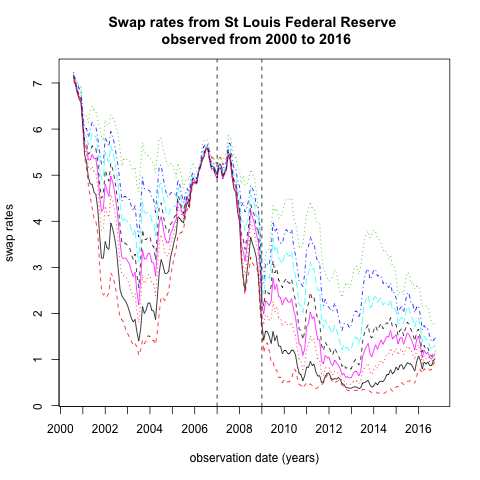
\includegraphics[width=0.75\textwidth]{gfx/chapter-yc-insurance/forecasting_graph6}
% figure caption is below the figure
\caption{Swap rates data (in \%) from St Louis Federal Reserve Bank, at maturities $1, 2, 3, 4, 5, 7, 10, 30$}
\label{forecast:6}       % Give a unique label
\end{figure}


\begin{table}
\begin{center}
% table caption is above the table
\caption{Descriptive statistics for St Louis Federal Reserve data}
\label{tab:freddatatables1}       % Give a unique label
% For LaTeX tables use
\begin{tabular}{lllllll}
\hline\noalign{\smallskip}
Maturity & Min. & 1st Qrt & Median & Mean & 3rd Qrt & Max.\\
\noalign{\smallskip}\hline\noalign{\smallskip}
  1  & 0.0026 & 0.0050  & 0.0134  & 0.0211  & 0.0336  & 0.0705\\
  2  & 0.0037 & 0.0078  & 0.0182  & 0.0239  & 0.0390  & 0.0712\\
  3  & 0.0046 & 0.0108  & 0.0236  & 0.0269  & 0.0422  & 0.0714\\
  4  & 0.0060 & 0.0134  & 0.0280  & 0.0296  & 0.0439  & 0.0715\\
  5  & 0.0078 & 0.0167  & 0.0316  & 0.0319  & 0.0456  & 0.0717\\
  7  & 0.0119 & 0.0215  & 0.0368  & 0.0354  & 0.0483  & 0.0720\\
  10 & 0.0139 & 0.0261  & 0.0419  & 0.0388  & 0.0502  & 0.0724\\
  30 & 0.0175 & 0.0327  & 0.0465  & 0.0440  & 0.0537  & 0.0720\\
\noalign{\smallskip}\hline
\end{tabular}
\end{center}
\end{table}

\medskip

We transformed these swap rates into zero rates by using a single curve calibration (that is, ignoring the counterparty credit risk) with linear interpolation between the maturities; one of the methods used in section ~\ref{andersen2010examples}. Then, as in the previous section, NS, NSS, CMN are used for fitting and forecasting the curves, with \code{auto.arima} applied to the factors. 

\medskip

We obtain 6-months and 36-months ahead forecasts,  from rolling training/testing windows (as in the last section) with respectively, a fixed  6 and 36 months length. The average out-of-sample RMSE are then calculated for each method, on the whole set of observed and forecasted yields. 

\medskip

The \textit{best} hyperparameters - associated with the lowest out-of-sample average RMSE - for each model are obtained through a search on a grid of values. For a 6-months horizon, they are (using the notations from section \ref{benchmarking}):
\begin{itemize}
\item NS: $\lambda = 1.6042$  
\item NSS: $\lambda_1 = 1.6250$ $\lambda_2 = 1.6250$
\item CMN: $a = 177.8279$, $\sigma = 3.9473e-04$, $K = 6$
\end{itemize}

and for a 36-months horizon: 
\begin{itemize}
\item NS: $\lambda = 1.4271$  
\item NSS: $\lambda_1 = 1.575$ $\lambda_2 = 1.575$
\item CMN: $a = 14.6780$, $\sigma = 0.0011$, $K = 4$
\end{itemize}

\medskip

The following results are obtained for the out-of-sample average RMSE: 

\begin{table}[!htb]
\begin{center}
% table caption is above the table
\caption{Descriptive statistics for out-of-sample RMSE, for training window = 6 months, and testing window = 6 months}
\label{tab:freddatatables3}       % Give a unique label
% For LaTeX tables use
\begin{tabular}{llllllll}
\hline\noalign{\smallskip}
Method & Min. & 1st Qrt & Median & Mean & 3rd Qrt & Max. & Std. Dev\\
\noalign{\smallskip}\hline\noalign{\smallskip}
  NS   & 0.00101  & 0.00269  & 0.00409  & 0.00481  & 0.00595  & 0.01530 & 0.00296\\
  NSS  & 0.00102  & 0.00269  & 0.00411  & 0.00481  & 0.00595  & 0.01537 & 0.00296\\
  CMN  & 0.00115  & 0.00256  & 0.00396  & 0.00468  & 0.00580  & 0.01600 & 0.00302\\
\noalign{\smallskip}\hline
\end{tabular}
\end{center}
\end{table}

\begin{table}[!htb]
\begin{center}
% table caption is above the table
\caption{Descriptive statistics for out-of-sample RMSE, for training window = 36 months, and testing window = 36 months}
\label{tab:freddatatables4}       % Give a unique label
% For LaTeX tables use
\begin{tabular}{llllllll}
\hline\noalign{\smallskip}
Method & Min. & 1st Qrt & Median & Mean & 3rd Qrt & Max. & Std. Dev\\
\noalign{\smallskip}\hline\noalign{\smallskip}
  NS   & 0.00356  & 0.00703  & 0.01044  & 0.01489  & 0.01609  & 0.21500 & 0.0213\\
  NSS  & 0.00300  & 0.00690  & 0.01114  & 0.01484  & 0.01689  & 0.21570 & 0.0201\\
  CMN  & 0.00402  & 0.00945  & 0.01279  & 0.01452  & 0.01917  & 0.03710 & 0.0070\\
\noalign{\smallskip}\hline
\end{tabular}
\end{center}
\end{table}

Using tables \ref{tab:freddatatables3}, \ref{tab:freddatatables4} and figures \ref{forecast:7} and \ref{forecast:8}, we observe that CMN give results which are close to those from NS and NSS, with a lower average out-of-sample RMSE in both cases. For a training window equal to six months, and testing window of six months, the results obtained by the three methods are pretty similar, and the same performance is observed for the three during the financial crisis.  For a training and testing window of thirty six months length, CMN has a lower mean and standard deviation for out-of-sample RMSE overall, but doesn't perform the best in the period of financial crisis 2007-2009. 

%\newpage

\begin{figure}[!htb]
\centering
% Use the relevant command to insert your figure file.
% For example, with the graphicx package use
  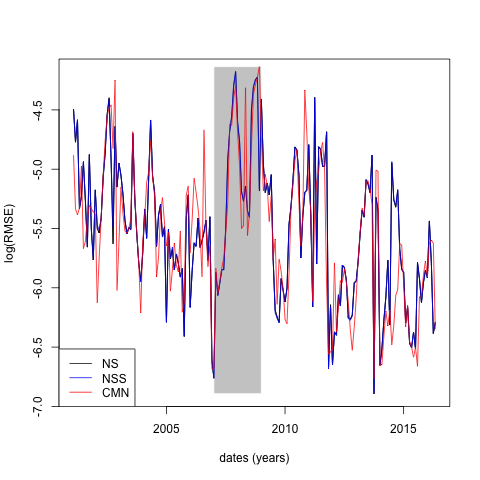
\includegraphics[width=0.65\textwidth]{gfx/chapter-yc-insurance/forecasting_graph7}
% figure caption is below the figure
\caption{log(out-of-sample RMSE) for training window = 6 months, and testing window = 6 months}
\label{forecast:7}       % Give a unique label
\end{figure}

\begin{figure}[!htb]
\centering
% Use the relevant command to insert your figure file.
% For example, with the graphicx package use
  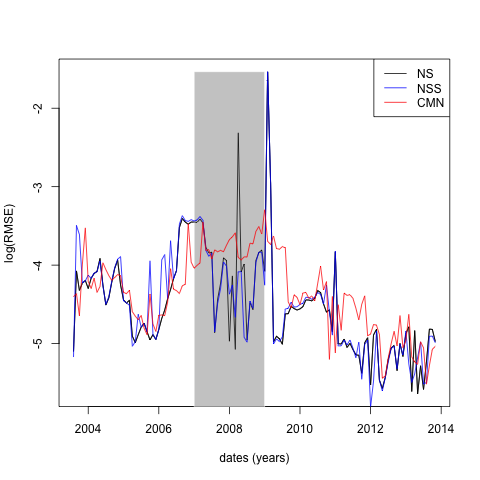
\includegraphics[width=0.65\textwidth]{gfx/chapter-yc-insurance/forecasting_graph8}
% figure caption is below the figure
\caption{log(out-of-sample RMSE) for training window = 36 months, and testing window = 36 months}
\label{forecast:8}       % Give a unique label
\end{figure}

\section{Conclusion}

In this paper, we introduced a method for swap discount curve construction and extrapolation. This method relies on the closed form formulas for discount factors available in exogenous short-rate models. We presented different ways to calibrate and extrapolate the model on different data sets from the existing literature. Moreover, we showed that the model's parameters contain a certain predictive power, enabling to obtain swap curves' forecasts, with predictive distribution.


\newpage

\section{Appendix}

\subsection{Data from \cite{andersen2010interest}}

\medskip
\begin{center}
\begin{tabular}{|l|c|r|}
  \hline
  Maturity & Swap Par Rate \\
  \hline
  1 & 4.20\% \\
  2 & 4.30\%  \\
  3 & 4.70\%  \\
  5 & 5.40\%  \\
  7 & 5.70\%  \\
  10 & 6.00\%  \\
  12 & 6.10\%  \\
  15 & 5.90\%  \\
  20 & 5.60\%  \\
  25 & 5.55\%  \\
  \hline
\end{tabular}
\end{center}

\subsection{Data from \cite{andersen2007discount}}

\medskip
\begin{center}
\begin{tabular}{|l|c|r|}
  \hline
  Maturity & Swap Par Rate \\
  \hline
  0.5 & 2.75\% \\
  1 & 3.10\%  \\
  1.5 & 3.30\%  \\
  2 & 3.43\%  \\
  2.5 & 3.53\%  \\
  3 & 3.30\%  \\
  4 & 3.78\%  \\
  5 & 3.95\%  \\
  7 & 4.25\%  \\
  10 & 4.50\%  \\
  12 & 4.65\%  \\
  15 & 4.78\%  \\
  20 & 4.88\%  \\
  30 & 4.85\%  \\
  \hline
\end{tabular}
\end{center}

\subsection{Data from \cite{hagan2006interpolation}}

\medskip
\begin{center}
\begin{tabular}{|l|c|r|}
  \hline
  Maturity & Continuous yield \\
  \hline
  0.1 & 8.10\% \\
  1 & 7.00\%  \\
  4 & 4.40\%  \\
  9 & 7.00\%  \\
  20 & 4.00\%  \\
  30 & 3.00\%  \\
  \hline
\end{tabular}
\end{center}


\subsection{Data from \cite{ametrano2013everything}}

\medskip
\begin{center}
\begin{tabular}{|l|c|r|}
  \hline
  Maturity & EUR6M IRS & Eonia OIS  \\
  \hline
  1 & 0.286\% & 0.000\% \\
  2 & 0.324\%  & 0.036\% \\
  3 & 0.424\%  & 0.127\% \\
  4 & 0.576\%  & 0.274\% \\
  5 & 0.762\%  & 0.456\% \\
  6 & 0.954\%  & 0.647\% \\
  7 & 1.135\%  & 0.827\% \\
  8 & 1.303\%  & 0.996\% \\
  9 & 1.452\%  & 1.147\% \\
  10 & 1.584\%  & 1.280\% \\
  11 & 1.703\%  & 1.404\% \\
  12 & 1.809\%  & 1.516\% \\
  13 & 1.901\%  & - \\
  14 & 1.976\%  & - \\
  15 & 2.037\%  &  1.764\%\\
  16 & 2.086\%  & - \\
  17 & 2.123\%  & - \\
  18 & 2.150\%  & - \\
  19 & 2.171\%  & - \\
  20 & 2.187\%  & 1.939\% \\
  21 & 2.200\%  & - \\
  22 & 2.211\%  & - \\
  23 & 2.220\%  & - \\
  24 & 2.228\%  & - \\
  25 & 2.234\%  & 2.003\% \\
  26 & 2.239\%  & - \\
  27 & 2.243\%  & - \\
  28 & 2.247\%  & - \\
  29 & 2.251\%  & - \\
  30 & 2.256\%  & 2.038\% \\
  35 & 2.295\%  & - \\
  40 & 2.348\%  & - \\
  50 & 2.421\%  & - \\
  60 & 2.463\%  & - \\
  \hline
\end{tabular}
\end{center}
 % INCLUDE: yc-insurance
%\forcenewpage

<<<<<<< HEAD
% !TEX root = ../moudiki_thesis.tex
%
\chapter{Multiple time series forecasting using quasi-randomized functional link neural networks}
\label{sec:rvfl_mts}

\section{Introduction}

In this chapter, we are interested in obtaining forecasts for multiple time series, by taking into account the potential nonlinear relationships between their observations. This type of problem has been tackled recently by \cite{exterkate2016nonlinear}, who applied kernel regularized least squares to a set of macroeconomic time series. The Long Short-Term Memory neural networks (LSTM) architectures (introduced by \cite{hochreiter1997long}) are another family of models, which are currently widely used for this purpose. As a basis for our model, we will use (quasi-)randomized neural networks known as Random Vector Functional Link neural networks (RVFL networks hereafter)

\medskip

The forecasting method described in this chapter, provides useful inputs for Insurance quantitative Risk Management models; the interested reader can refer to \cite{bonnin2015retraite} for example.

\medskip

To the best of our knowledge, randomized neural networks were introduced by \cite{schmidt1992feedforward}, and the RVFL networks were introduced by \cite{pao1994learning}. An early approach for multivariate time series forecasting using neural networks is described in \cite{chakraborty1992forecasting}. They applied a \textit{back propagation} algorithm from \cite{rumelhart1988learning} to trivariate time series, and found that the combined training of the series gave better forecasts than a separate training of each individual series. The novelty of the approach described in this chapter is to derive an RVFL model for multiple time series, under two separate regularization constraints on the parameters, as it will be described in details in  section ~\ref{solve_rvfl}.

\medskip

RVFL networks are \textit{multilayer feedforward} neural networks, in which there is a \textit{direct link} between the predictors and the output variable, aiming at capturing the linear relationships. In addition to the \textit{direct link}, there are new features: the hidden nodes (the dataset is augmented), that help to capture the nonlinear relationships between the time series. These new features are obtained by random simulation over a given interval. More details on the \textit{direct link} and the hidden nodes will be provided in the next section.

\medskip

The RVFL networks have been successfully applied to solving different types of classification and regression problems; see for example \cite{dehuri2010comprehensive}. More specifically, they have been applied to univariate time series forecasting by \cite{ren2016random}. A comprehensive survey can be found in \cite{zhang2016comprehensive}; where a large number of model specifications are tested on classification problems, including changing the range of hidden layer's randomization.

\medskip

Here, we will use RVFL networks with one hidden layer. And instead of relying on fully randomized nodes, we will use sequences of deterministic quasi-random numbers. Indeed, with fully randomized nodes, the model fits obtained are dependent on the choice of a simulation \textit{seed}. Typically, a different fitting solution would be obtained for each \textit{seed}.

\medskip

In our various numerical examples from section \ref{sec:numericalexamples}, we will apply the RVFL networks to forecasting trivariate time series, notably (but not only) in a Dynamic Nelson Siegel (DNS) framework (see \cite{nelson1987parsimonious}, \cite{diebold2006forecasting}). We will obtain point forecasts and predictive distributions  for the series, and see that in this RVFL framework, one (or more) variable(s) can be stressed, and influence the others. More precisely, about this last point, it means that it is possible, as in dynamic regression models (\cite{pankratz2012forecasting}) to assign a specific future value to one regressor, and obtain forecasts of the remaining variables. Another advantage of the model described here, is its ability to integrate multiple other exogenous variables, without overfitting in-sample data.

\section{Description of the model}

The general procedure for obtaining the model's optimal parameters and predictions is  summarized in figure \ref{fig:flowchart}.

\begin{figure}[!htb]
\centering
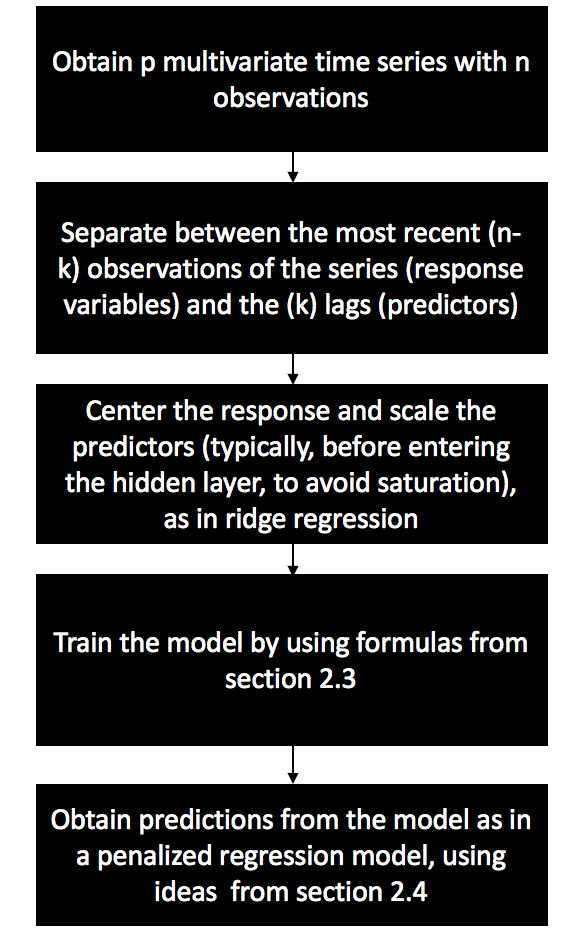
\includegraphics[width=5.5cm]{gfx/chapter-rvfl-mts/flowchart}
\caption{}
\label{fig:flowchart}
\end{figure}


This procedure is described in details in the next sections, especially sections \ref{solve_rvfl} and \ref{sec:preds}.

\clearpage

\subsection{On a single layer RVFL networks}
\label{sec:modeldesc}

We rely on single layer feed forward neural networks (SLFN).
Considering that an output variable $y \in \RR^n$ is to be explained by a set of observed predictors $Z^{(j)} \in \RR^n$, $j \in \left\lbrace 1, \ldots,
p\right\rbrace$, the RVFL networks we will use to explain $y$ can be described for $i \in \left\lbrace 1, \ldots, n\right\rbrace$ as:
$$
y_i = \beta_0 + \sum_{j = 1}^p \beta_j Z_i^{(j)} + \sum_{l = 1}^L \gamma_l \:
g\left(\sum_{j = 1}^p W^{(j, l)} Z_i^{(j)}\right) + \epsilon_i
$$

\medskip

$g$ is called \textit{activation function}, $L$ is the number of nodes in the hidden
layer, $W^{(j, l)}$ are elements of the hidden layer, and the parameters
$\beta_j$ and $\gamma_l$ are to be learned from the observed data $Z^{(j)}, \: j
\in \left\lbrace 1, \ldots, p\right\rbrace$. The $\epsilon_i$'s are the residual
differences between the output variable values and the RVFL model.

\medskip

This type of model can be seen as a one explaining $y_i$, by finding a
compromise between linear and potentially non-linear effects of the original
predictors $Z^{(j)}$ and transformed predictors
$$
\Phi(\textbf{Z})^{(l)}= g\left(\sum_{j = 1}^p W^{(j, l)} Z_i^{(j)}\right)
$$
$\left \lbrace 1, \ldots, L\right\rbrace$ on the response. Common choices for function $g$ in neural networks regression are the sigmoïd activation function
$$
g: \: x \mapsto \frac{1}{1 + e^{-x}}
$$
the hyperbolic tangent function,
$$
g: \: x \mapsto tanh(x) = \frac{e^x - e^{-x}}{e^x + e^{-x}}
$$
or the Rectified Linear Units, known as ReLU
$$
g: \: x \mapsto max(x, 0)
$$

\medskip

The main differences between the RVFL framework and a \textit{classical} SLFN framework are:

\begin{itemize}
\item The inclusion of a linear dependence between the output variable and the
predictors: the \textit{direct link}, $\beta_0 + \sum_{j = 1}^p \beta_j Z_i^{(j)}$
\item The elements $W^{(j, l)}$ of the hidden layer are typically not trained, but randomly and uniformly chosen on a given interval. Different ranges for these elements of the hidden layer are tested in \cite{zhang2016comprehensive}).
\end{itemize}

\medskip

Solving for the optimal parameters $\beta_j$'s and $\gamma_l$'s can be done by applying directy a least squares regression of $y$ on the set of observed and transformed predictors. But since these input predictors are likely to be highly correlated - especially in our setting, with time series data - we do not search each of these parameters on the entire line, but in restricted regions
where we have:
$$
\sum_{j=1}^p \beta_j^2  \leq u
$$
and
$$
\sum_{l=1}^L
\gamma_l^2 \leq v
$$ for $u, v \in \RR^*$. That is, applying some kind of Tikhonov regularization or ridge regression model (\cite{hoerl1970ridge}) of $y$ on the set of observed and transformed predictors. Having two constraints instead of one, allows for more flexibility in the covariance structure between the predictors and the output, with $\beta_j$'s and $\gamma_l$'s moving in separate balls. For these constraints to be applicable, the input variables will need to be standardized, so as to be expressed on the same scales, and the response variable will be centered.

\medskip

Imposing these restrictions to the model's parameters increases their interpretability - by reducing their variance -, at the expense of a slight increase in in-sample bias. It also prevents the model from overfitting the data as in ridge regression (\cite{hoerl1970ridge}). One of the advantages of RVFL networks is that they are relatively fast to train, due to the availability of closed-form formulas for the model's parameters, as it will be presented in the next section.

\medskip

On the other hand, RVFL networks incorporate some randomness in the hidden layer, which makes each model relatively dependent on the choice of a simulation \textit{seed}. Each \textit{seed} would indeed produce a different set of parameters $\beta_j$'s and $\gamma_l$'s for the model. For that reason, we will also use sequences of deterministic quasi-random numbers in the hidden layer. The elements $W^{(j, l)}$ of the hidden layer are taken from a quasi-random (deterministic) \textit{sobol} sequence on $[0, 1]$, which is shifted in such a way that they belong to $[-1, 1]$.

\medskip

\textit{Sobol} sequences are part of quasi-random numbers, which are also called \textit{low discrepancy} sequences. As described intuitively in \cite{boyle1997quasi}, the discrepancy of a sequence of $N$ points in a subcube $V \in [0, 1)^d$ is defined as:
$$
sup_{V \in [0, 1)^d} |\frac{number \: of \: points \: in \: V}{N} - v(V)|
$$
where $v(V)$ is the volume of $V$. It describes how well the points are dispersed within $V$. The idea is to have points which are more or less equidispersed in $V$. \cite{joe2008sobol} describe the generation of the $i^{th}$ term, $j^{th}$ component ($x_{i, j}$) of a Sobol sequence. The generation starts with obtaining the binary representation of $i$. That is, obtaining $i$ as:
$$
i = \sum_k i_k 2^k = ( \ldots \: i_3 \: i_2 \: i_1)_2
$$

For example, $5 = 1 \times 2^2 + 0 \times 2^1 + 1 \times 2^0$ can be expressed as $(101)_2$ in binary representation. Then, by using the sequence of bits describing $i$ in base $2$, we can obtain $x_{i, j}$ as:

\begin{equation}
\label{ithjthsobol}
x_{i, j} = i_1 v_{1, j} \oplus i_2 v_{2, j} \oplus \ldots
\end{equation}

Where $\oplus$ is a bitwise exclusive-or operation, and the numbers $v_{i, j}$ are called the direction numbers, defined for $k \geq 1$ as:

\begin{equation}
\label{directionv}
v_{k, j} = \frac{m_{k, j}}{2^k} = \frac{2 a_{1, j} m_{k-1, j} \oplus 2^2 a_{2, j}m_{k-2, j} \oplus \ldots \oplus 2^{s_j - 1} a_{s_j - 1, j}m_{k-s_j+1, j} \oplus 2^{s_j} m_{k-s_j, j} \oplus m_{k-s_j, j}   }{2^k}
\end{equation}

A few details on equation \ref{directionv}:

\begin{itemize}
\item The bitwise exclusive-or operation $\oplus$ applied to two integers $p$ and $q \in \left \lbrace 0, 1 \right \rbrace$ returns $1$ if and only if one of the two (but not both) inputs is equal to $1$. Otherwise, $p \oplus q$ is equal to 0.
\item The second term of the equation relies on primitive polynomials of degree $s_j$, with coefficients $a_{i, j}$ taken in $\left \lbrace 0, 1 \right \rbrace$:
\begin{equation}
\label{primitivepoly}
x^{s_j} + a_{1, j} x^{s_j - 1} + a_{2, j} x^{s_j - 2} + \ldots + a_{s_j - 1, j} x + 1
\end{equation}
\item The terms $m_{k, j}$ are obtained recursively, with the initial values  $m_{1, j}, m_{2, j}, \ldots, m_{k - s_j, j}$ chosen freely, under the condition that $m_{k, j}, 1 \leq k \leq s_j$ is odd and less than $2^k$.
\end{itemize}

A more complete treatment of \textit{low discrepancy} sequences can be found in \cite{niederreiter1992random}. And an example with $s_j = 3$, $a_{1, j} = 0$, $a_{2, j} = 1$ is given in \cite{joe2008sobol}.

\subsection{Applying RVFL networks to multivariate time series forecasting}
\label{apply_rvfl}

We consider $p \in \mathbb{N}^*$ time series $(X_t^{(j)})_{t \geq 0}, j = 1, \ldots, p$,
observed at $n \in \mathbb{N}^*$ discrete dates. We are interested in
obtaining simultaneous forecasts of the $p$ time series at time $n+h$, $h \in
\mathbb{N}^*$, by allowing each of the $p$ variables to be influenced by the
others (in the spirit of VAR models, see \cite{lutkepohl2005new}).

\medskip

For this purpose, we use $k < n$ lags of each of the observed $p$ time
series. The output variables to be explained are:

\begin{equation}
Y^{(j)} = \left(X^{(j)}_n, \ldots, X^{(j)}_{k+1} \right)^T
\end{equation}

for $j \in \left\lbrace 1, \ldots,
p \right\rbrace$. Where $X^{(j)}_n$ is the most contemporaneous observed value
of the $j^{th}$ time series, and $X^{(j)}_{k+1}$ was observed $k$ dates earlier
in time for $(X^{(j)}_t)_{t \geq 0}$. These output variables are stored in a
matrix: $$ \bfY \in \RR^{(n-k) \times p} $$ and the predictors are
stored in a matrix: $$ \bfX \in \RR^{(n-k) \times (k \times p)} $$
where $\bfX$ consists in $p$ blocks of $k$ lags, for each one of the observed
$p$ time series. For example, the $j_0^{th}$ block of ${\bf X}$, for $j_0 \in
\left\lbrace 1, \ldots, p \right\rbrace$  contains in columns:

\begin{equation}
\left( X^{(j_0)}_{n-i}, \ldots, X^{(j_0)}_{k+1-i} \right)^T
\end{equation}

with $i \in
\left\lbrace 1, \ldots, k \right\rbrace$. It is also possible to add other
regressors, such as dummy variables, indicators of special events, but for
clarity, we consider only the inclusion of lags.

\medskip

As described in the previous section, an additional layer of transformed  predictors is added to $\bfX$, in order to capture the potentially non-linear
interactions between the predictors and the output variable. Adding the transformed predictors to the original ones, leads to a new matrix of predictors with
dimensions $(n-k) \times (k \times p + L)$, where $L$ is the number of nodes in
the hidden layer. We are then looking for simultaneous predictions $$ \hat{X}^{(j)}_{n+h|n, \ldots, 1} =:
\hat{X}^{(j)}_{n+h} $$ for $h \in \mathbb{N}^*$, and $j \in \left\lbrace 1,
\ldots, p \right\rbrace$. This, is a \textit{multi-task learning} problem (see \cite{caruana1998multitask}), in which the output variables will all share the same set of predictors.

\medskip

For example, we have $p = 2$ time series $(X^{(1)}_{t_1}, \ldots,  X^{(1)}_{t_5})$ and $(X^{(2)}_{t_1}, \ldots,  X^{(2)}_{t_5})$ observed at $n = 5$ dates $t_1 < \ldots < t_5$, with $k = 2$ lags, and $L = 3$ nodes in the hidden layer. In this case, the response variables are stored in:
$$
\bfY = \left( {\begin{array}{cc} X^{(1)}_{t_5} &  X^{(2)}_{t_5}\\ X^{(1)}_{t_4} & X^{(2)}_{t_4} \\ X^{(1)}_{t_3} & X^{(2)}_{t_3}\      \end{array} } \right)
$$
The predictors are stored in:
$$
\bfX = \left( {\begin{array}{cccc} X^{(1)}_{t_4} & X^{(1)}_{t_3} & X^{(2)}_{t_4} & X^{(2)}_{t_3} \\ X^{(1)}_{t_3} & X^{(1)}_{t_2} & X^{(2)}_{t_3} & X^{(2)}_{t_2} \\ X^{(1)}_{t_2} & X^{(1)}_{t_1} & X^{(2)}_{t_2} & X^{(2)}_{t_1} \      \end{array} }\right)
$$
And the coefficients in the hidden layer are:
$$
\textbf{W} = \left( {\begin{array}{ccc} W^{(1, 1)} & W^{(1, 2)} & W^{(1, 3)}  \\ W^{(2, 1)} & W^{(2, 2)} & W^{(2, 3)}  \\ W^{(3, 1)} & W^{(3, 2)} & W^{(3, 3)} \\ W^{(4, 1)} & W^{(4, 2)} & W^{(4, 3)}  \      \end{array} }\right)
$$

\subsection{Solving for $\hat{\beta}$'s and $\hat{\gamma}$'s}
\label{solve_rvfl}

We let $y$ be the $j_0^{th}$ column (out of $p$) of the response matrix $\bfY$, and $\Phi(\bfX)$ be the matrix of transformed predictors obtained from $\bfX$ by the hidden layer described at the beginning of section \ref{sec:modeldesc}. We also denote the set of regression parameters associated with this $j_0^{th}$ time series, as:
$$
\beta_m^{(j_0)} =: \beta_m
$$
and
$$
\gamma_l^{(j_0)} =: \gamma_l
$$

for $m \in \left\lbrace 1, \ldots, k \right\rbrace$; $l \in \left\lbrace 1, \ldots,  L\right\rbrace$. Solving for the regression parameters for the $j_0^{th}$ time series, under the constraints
$$
\sum_{m=1}^{k\times p} \beta_m^2 \leq u
$$
and
$$
\sum_{l=1}^L \gamma_l^2 \leq v
$$
for $u, v \in \RR^*$, leads to minimizing a penalized residual sum of squares. Hence, for vectors $\beta \in  \RR^{(k \times p)}$ and $\gamma \in  \RR^L$ containing the regression parameters, we obtain the Lagrangian:
$$
\mathcal{L}(\bfX; \beta, \gamma) = \left(y - \bfX\beta -
\Phi(\bfX)\gamma\right)^T\left(y - \bfX\beta - \Phi(\bfX)\gamma\right) + \lambda_1
\beta^T \beta + \lambda_2 \gamma^T\gamma
$$

\medskip

where $\lambda_1$ and $\lambda_2$ are Lagrange multipliers.  Taking the first derivatives of $\mathcal{L}$ relative to $\beta$ and $\gamma$ leads to:

\begin{eqnarray*}
\frac{\partial \mathcal{L}(\bfX;\beta, \gamma)}{\partial
\beta}
&=& - y^T\bfX - \bfX^Ty + 2 (\bfX^T\bfX)\beta + \bfX^T
\Phi(\bfX)\gamma + \left(\Phi(\bfX)\gamma\right)^T \bfX + 2\lambda_1 \beta \\
&=& 2 (\bfX^T\bfX + \lambda_1 I_{k\times p})\beta - y^T\bfX - \bfX^Ty + \bfX^T \Phi(\bfX)\gamma +
\left(\Phi(\bfX)\gamma\right)^T \bfX \\
&=& 2 (\bfX^T\bfX + \lambda_1 I_{k\times p})\beta -
2 \bfX^Ty + 2 \bfX^T \Phi(\bfX)\gamma
\end{eqnarray*}

where $I_{k\times p}$ is the identity matrix with dimensions $(k\times p) \times (k\times p)$ and equivalently

\begin{eqnarray*}
\frac{\partial
\mathcal{L}(\bfX;\beta, \gamma)}{\partial \gamma} &=& 2 (\Phi(\bfX)^T\Phi(\bfX) + \lambda_2
I_{L})\gamma -2 \Phi(\bfX)^Ty + 2 \Phi(\bfX)^T\bfX\beta
\end{eqnarray*}

where $I_L$ is the identity matrix with dimensions $L \times L$. And setting these first derivatives to $0$ leads to:
$$
\left\{ \begin{array}{c}
(\bfX^T\bfX + \lambda_1 I_{k\times p})\beta  +  \bfX^T \Phi(\bfX)\gamma =  \bfX^Ty \\
(\Phi(\bfX)^T\Phi(\bfX) + \lambda_2 I_{L})\gamma +  \Phi(\bfX)^T\bfX\beta =  \Phi(\bfX)^Ty
\end{array} \right.
$$

That is:
$$
\left( {\begin{array}{cc} \bfX^T\bfX + \lambda_1 I_{k\times p} &
\bfX^T\Phi(\bfX)\\ \Phi(\bfX)^T\bfX & \Phi(\bfX)^T\Phi(\bfX) + \lambda_2 I_{L} \      \end{array}
} \right) \left( {\begin{array}{c} \beta \\       \gamma \      \end{array} }
\right) = \left( {\begin{array}{c} \bfX^Ty \\       \Phi(\bfX)^Ty \      \end{array} }
\right)
$$

Now, if we denote:

$$ A = \left( {\begin{array}{cc} \bfX^T\bfX + \lambda_1 I_{k\times p} &  \bfX^T\Phi(\bfX)\\
\Phi(\bfX)^T\bfX & \Phi(\bfX)^T\Phi(\bfX) + \lambda_2 I_{L} \      \end{array} } \right) =:
\left( {\begin{array}{cc} B &  C^T\\ C & D \      \end{array} } \right) $$

and $S = D - CB^+C^T$. Then, using the algorithm described in \cite{cormen2009introduction} for blockwise matrix inversion, we obtain: $$ A^+ = \left( {\begin{array}{cc} B^+ + B^+ C^T
S^+ CB^+  &  -B^+ C^T S^+\\ -S^+CB^+ & S^+ \      \end{array} } \right) =:
\left( {\begin{array}{cc} A_1^+  &  A_2^+\\ A_3^+ & A_4^+ \      \end{array} }
\right) $$


where $S^+$ and $B^+$ are the Moore-Penrose pseudo-inverse (\cite{penrose1955generalized}) of matrixes $S$ and
$B$. Hence for each column $y$ of $\bfY$, we have the solutions:

$$
\left( {\begin{array}{c} \hat{\beta} \\       \hat{\gamma} \      \end{array}
} \right) = \left( {\begin{array}{cc} A_1^+  &  A_2^+\\ A_3^+ & A_4^+ \
\end{array} } \right)\left( {\begin{array}{c} \bfX^Ty \\       \Phi(\bfX)^Ty \
\end{array} } \right)
$$

And the whole set of parameters, for all the $p$ observed time series is given by:

$$
\left( {\begin{array}{c} \hat{\underline{\beta}} \\       \hat{\underline{\gamma}} \      \end{array}
} \right) := \left( {\begin{array}{cc} A_1^+  &  A_2^+\\ A_3^+ & A_4^+ \      \end{array}
} \right)\left( {\begin{array}{c} \bfX^T\bfY \\       \Phi(\bfX)^T\bfY \      \end{array} }
\right)
$$

The objective function to be minimized (the least squares) is convex, and so is the set of feasible solutions. The solutions ${\hat{\underline{\beta}}}$ and ${\hat{\underline{\gamma}}}$ found here, are hence global minima.

\subsection{h-steps ahead forecasts and use of dynamic regression}
\label{sec:preds}

Having obtained the optimal set of parameters
$\hat{\underline{\beta}}$ and $\hat{\underline{\gamma}}$ as described in the previous section,  a new set of predictors is constructed by using the former output variables contained in response matrix $\bfY$'s columns. The first $k$ elements of each one of the $p$ columns of $\bfY$, which are the most contemporaneous values of the $p$ series, constitute the new predictors.

\medskip

Hence, if we denote the new predictors as:
\begin{eqnarray}
\bfX^*_n &=& \left(X^{(1)}_n, \ldots, X^{(1)}_{n-k+1}, \ldots, \ldots, X^{(p)}_n, \ldots, X^{(p)}_{n-k+1}\right)
\end{eqnarray}

The 1-step ahead forecasts are obtained as:

$$
\left(\hat{X}_{n+1}^{(1)}, \ldots, \hat{X}_{n+1}^{(p)}\right) =
\left(\bfX^*_n   \: \: \: \: \Phi(\bfX^*_n)\right) \left( {\begin{array}{c} \hat{\underline{\beta}} \\       \hat{\underline{\gamma}} \      \end{array}
} \right)
$$

The h-step ahead forecasts are obtained in a similar fashion; with the new forecasts $\left(\hat{X}_{n+1}^{(1)}, \ldots, \hat{X}_{n+1}^{(p)}\right)$ being added to the set of most contemporaneous values of the $p$ series, and used as part of the new predictors.

\medskip

In order to obtain confidence intervals around the point forecasts, we fit an ARIMA model to the in-sample residuals $\epsilon_i$ of each one of the $p$ time series, as in dynamic regression models (see \cite{pankratz2012forecasting}). An illustration can be found in the next section. Other models for the autocorrelated residuals could be envisaged, though.

\section{Numerical examples}
\label{sec:numericalexamples}

\subsection{A Dynamic Nelson-Siegel example}
\label{section:dnsexample1}

The following examples are not exhaustive benchmarks, but aim at illustrating the forecasting capabilities of the model described in this chapter. All the results on RVFL use the ReLU activation function. We use calibrated discount rates data from \href{http://www.bundesbank.de/Navigation/EN/Statistics/Time_series_databases/time_series_databases.html}{Deutsche Bundesbank website}, observed on a monthly basis, from the beginning of 2002 to the end 2015. There are 167 curves, observed at 50 maturities in the dataset. We obtain curves' forecasts in a Dynamic Nelson Siegel \cite{nelson1987parsimonious} framework (DNS), in the spirit of \cite{diebold2006forecasting} and other similar models \footnote{\cite{diebold2013yield}: \textit{"there are by now literally hundreds of DNS applications involving model fitting and forecasting"}}.

\medskip

In figure ~\ref{db_zerorates}, we present the data that we use, and table ~\ref{tab:summary_db_zeros} contains a summary of these data; the minimum, maximum, median, first and third quartiles of the discount rates observed at given maturities. There are alternate cycles of increases and decreases of the discount rates, with generally a decreasing trend. Some of the discount rates, at the most recent dates, and lower maturities, are negative.

\begin{figure}[!htb]
\centering
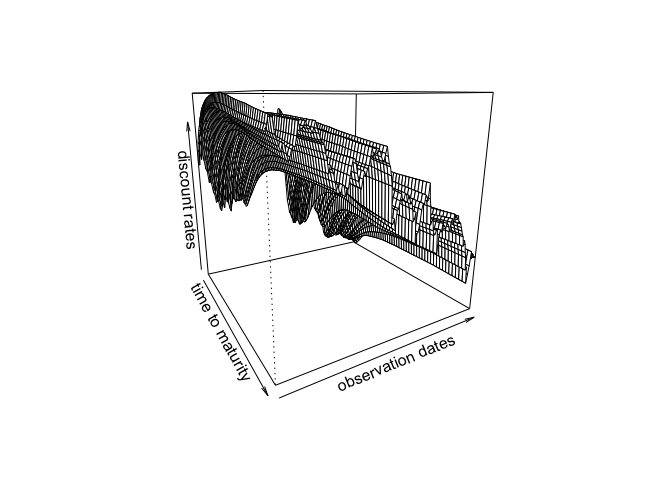
\includegraphics[width=14cm]{gfx/chapter-rvfl-mts/bundesbank_dR.png}
\caption{Observed discount rates from Deutsche Bundesbank website, from 2002 to the end 2015}
\label{db_zerorates}
\end{figure}

\begin{table}
\begin{center}
% table caption is above the table
\caption{Summary of observed discount rates from Deutsche Bundesbank website, from 2002 to the end 2015}
\label{tab:summary_db_zeros}       % Give a unique label
% For LaTeX tables use
\begin{tabular}{llllll}
\hline\noalign{\smallskip}
Maturity & Min & 1st Qrt  & Median  & 3rd Qrt  & Max  \\
\noalign{\smallskip}\hline\noalign{\smallskip}
  1 & -0.116 & 0.858 & 2.045 & 3.072 & 5.356 \\
  5 & 0.170 & 1.327 & 2.863 & 3.807 & 5.146\\
  15 & 0.711 & 2.616 & 3.954 & 4.702 & 5.758\\
  30 & 0.805 & 2.594 & 3.962 & 4.814 & 5.784\\
  50 & 0.749 & 2.647 & 3.630 & 4.590 & 5.467\\
\noalign{\smallskip}\hline
\end{tabular}
\end{center}
\end{table}

In the DNS framework, the spot interest rates observed at time $t$, for time to maturity $\tau$ are modeled as:
\begin{equation}
R_t(\tau) = \alpha_{1, t} + \alpha_{2, t}\left(\frac{1-e^{-\tau/\lambda}}{e^{-\tau/\lambda}}\right) + \alpha_{3, t}\left(\frac{1-e^{-\tau/\lambda}}{e^{-\tau/\lambda}} - e^{-\tau/\lambda}\right)
\end{equation}

\medskip

The factor loadings $1$, $\left(\frac{1-e^{-T/\lambda}}{e^{-T/\lambda}}\right)$ and $\left(\frac{1-e^{-T/\lambda}}{e^{-T/\lambda}} - e^{-T/\lambda}\right)$ are used to represent the level, slope, and curvature of the Yield Curve. We obtain estimations of $\alpha_{i, t}, i = 1, \ldots, 3$ for each cross-section of yields by fixing $\lambda$, and doing a least squares regression on the factor loadings. The three time series $\alpha_{i, t}, i = 1, \ldots, 3$ associated to the loadings for each cross-section of yields, are those that we wish to forecast simultaneously, by using an RVFL model.

\medskip

This type of model (DNS) cannot be used for no-arbitrage pricing as is, but it could be useful for example, for \textit{stressing} the yield curve factors under the historical probability. It can however be made arbitrage-free, if necessary (see \cite{diebold2013yield}). We will benchmark the RVFL model applied to the three time series $\alpha_{i, t}, i = 1, \ldots, 3$, against ARIMA and VAR models. \cite{diebold2006forecasting} applied an autoregressive AR(1) model separately to each one of the parameters, $\alpha_{i, t}, i = 1, \ldots, 3$.

\medskip

We will apply to these parameters' series: an ARIMA model (\cite{hyndman2008automatic}), and a Vector Autoregressive model (VAR, see \cite{pfaff2008var} and \cite{lutkepohl2005new}); with the parameter $\lambda$ of the DNS factor loadings, used as an \textit{hyperparameter} for the time series cross-validation. In the RVFL and the VAR model, the number of lags is also used as an \textit{hyperparameter} for the cross-validation. For the RVFL, the most recent values of $\alpha_{i, t}, i = 1, \ldots, 3$ are stored in matrix $\bfY$, as described in section \ref{solve_rvfl}, ordered by \textit{date of arrival}, whereas matrix $\bfX$ contains the lags of the three series.

\medskip

A rolling forecasting methodology (see \cite{bergmeir2015note}) is implemented in order to obtain these benchmarks. A fixed 12 months-length window for training the model, and the following 12 months for testing, the origin of the training set is then advanced of 1 month, and the training/testing procedure is repeated. The measure of forecasting performance is the Root Mean Squared Error ($RMSE$).

\begin{figure}[!htb]
\centering
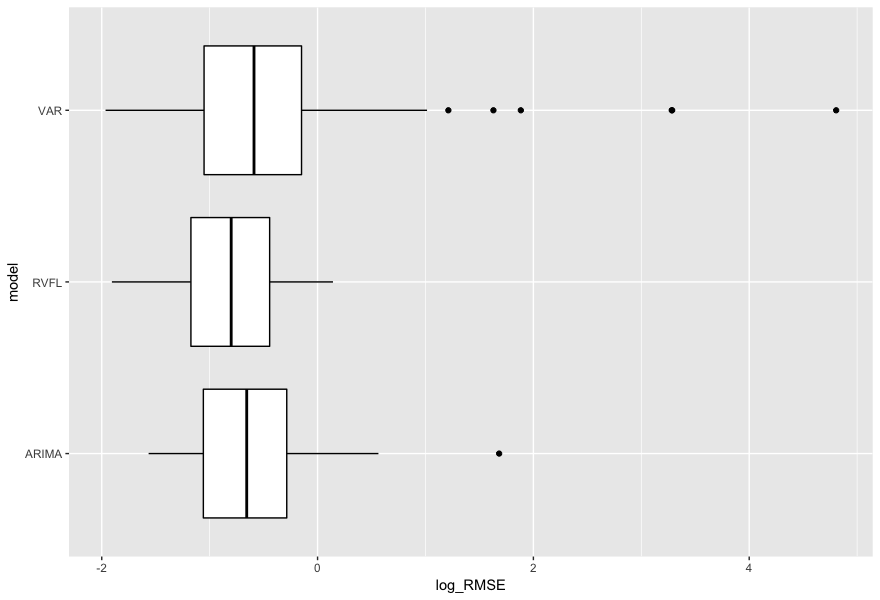
\includegraphics[width=10cm]{gfx/chapter-rvfl-mts/boxplot.png}
\caption{Distribution of out-of-sample $log(RMSE)$, for ARIMA, VAR, and RVFL}
\label{error_dist}
\end{figure}

\begin{figure}[!htb]
\centering
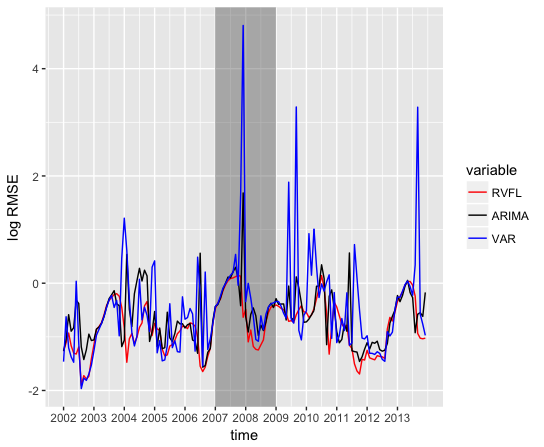
\includegraphics[width=10cm]{gfx/chapter-rvfl-mts/log_RMSE.png}
\caption{Out-of-sample $log(RMSE)$, for ARIMA, VAR, and RVFL over time}
\label{log_RMSE}
\end{figure}

Figure \ref{error_dist} presents boxplots for the distribution of out-of-sample errors obtained in the cross-validation procedure, and figure \ref{log_RMSE} presents the 12 months-ahead out-of-sample errors over time. ARIMA (separate (\cite{hyndman2008automatic}) ARIMA models applied to each series $\alpha_{i, t}, i = 1, \ldots, 3$) gives good results, as already suggested by  \cite{diebold2006forecasting}. They are nearly comparable to results from RVFL, but a bit more volatile, with an outlier point observed on the $log(RMSE)$ box plot.

\medskip

The unrestricted VAR model results include more volatility than the two other methods on this specific  example, especially in the period of financial crisis going from 2007 to 2009, as seen on figure ~\ref{log_RMSE}. Table ~\ref{tab:benchmark} is to be read in conjuction with the $log(RMSE)$ box plot presented in figure ~\ref{error_dist}. It summarises the results obtained by the different methods on the out-of-sample $RMSE$. Table ~\ref{tab:confint} contains $95\%$ confidence intervals around the mean of the differences between the three methods.

\medskip

\begin{table}
\begin{center}
% table caption is above the table
\caption{Comparison of 12 months ahead out-of-sample $RMSE$, for the ARIMA, RVFL, and VAR}
\label{tab:benchmark}       % Give a unique label
% For LaTeX tables use
\begin{tabular}{lllllll}
\hline\noalign{\smallskip}
Method & Min & 1st Qrt  & Median & Mean  & 3rd Qrt  & Max  \\
\noalign{\smallskip}\hline\noalign{\smallskip}
  RVFL & 0.1487 & \textbf{0.3092} & \textbf{0.4491} & \textbf{0.5041} & \textbf{0.6414} & \textbf{1.1535} \\
  ARIMA & 0.2089 & 0.3470 & 0.5187 & 0.6358 & 0.7516 & 5.3798\\
  VAR & \textbf{0.1402} & 0.3493 & 0.5549 & 1.9522  & 0.8619 & 122.2214 \\
\noalign{\smallskip}\hline
\end{tabular}
\end{center}
\end{table}


\begin{table}
\begin{center}
% table caption is above the table
\caption{95\% confidence interval around the difference of out-of-sample $RMSE$}
\label{tab:confint}       % Give a unique label
% For LaTeX tables use
\begin{tabular}{lllllll}
\hline\noalign{\smallskip}
Method & Lower bound & Upper bound  & Mean \\
\noalign{\smallskip}\hline\noalign{\smallskip}
  RVFL - ARIMA & -0.2116 & -0.0518 & \textbf{-0.1317}\\
  RVFL - VAR & -3.1888 & 0.2927 & \textbf{-1.4480} \\
  ARIMA - VAR & -2.9937 & 0.3610 & \textbf{-1.3163} \\
\noalign{\smallskip}\hline
\end{tabular}
\end{center}
\end{table}

\medskip

Another advantage of RVFL over ARIMA or AR(1) in this context is that, it would be possible to add other variables to the RVFL regression, such as inflation, or dummy variables for external events, and combine their effects. It is also possible to stress one variable, and see the effects on the other variables, as presented in the appendix section \ref{fcst_ci}: the parameter $\alpha_{1, t}$ is increased (from $0.75$ to $1.25$) and decreased (from $0.75$ to $0.25$), and the other parameters $\alpha_{2, t}$ and $\alpha_{3, t}$ forecasts move slightly, consecutively to these \textit{stresses}. The corresponding median forecast curves for these stresses, and some additional ones, are presented in figure ~\ref{stressed_NS2}.

\begin{figure}
\centering
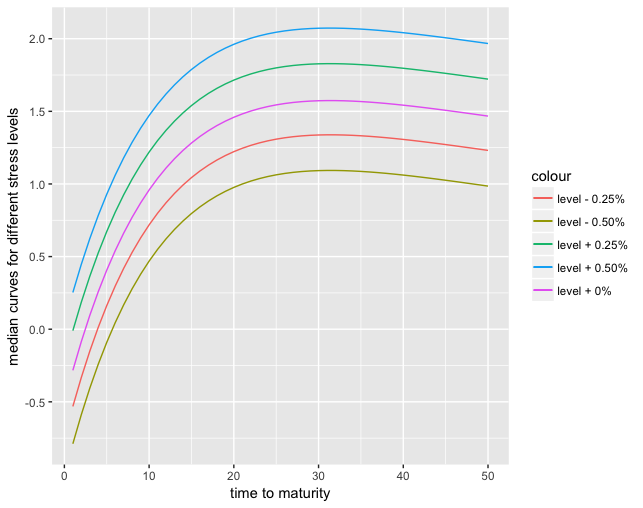
\includegraphics[width=11cm]{gfx/chapter-rvfl-mts/stressed_NS.png}
\caption{12 months-ahead median curves, for stressed yield curve level $\alpha_{1, t}$}
\label{stressed_NS2}
\end{figure}

\subsection{Forecasting 1 year, 10 years and 20 years spot rates}

For this second example, we forecast the 1-year, 10-years and 20-years spot rates time series from the previous dataset, on a 12-months horizon. As described in the previous section, we use a rolling forecasting methodology, with a training window of 12 months length.

\medskip

Figure \ref{ex2_data} presents the three time series of data, and a summary of the data can be found in tables \ref{tab:three_ts} and \ref{tab:three_ts_cor}.

\begin{figure}
\centering
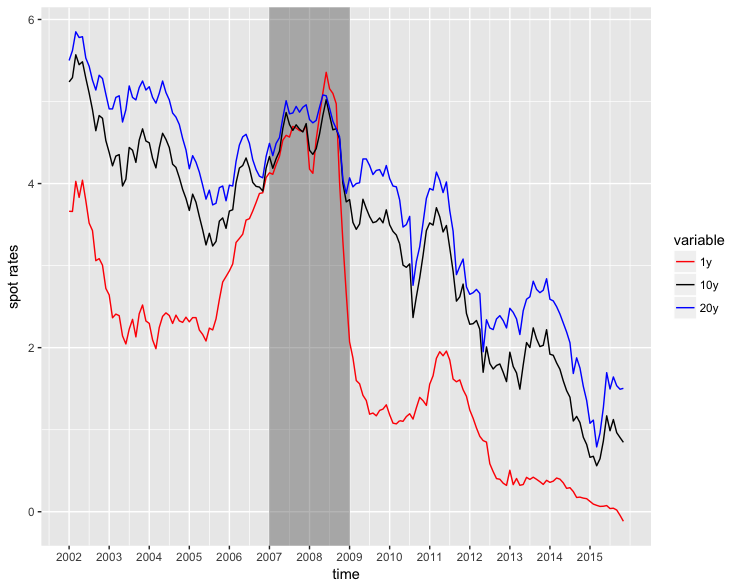
\includegraphics[width=12cm]{gfx/chapter-rvfl-mts/ex2_data.png}
\caption{1-year, 10-years and 20-years spot rates time series data}
\label{ex2_data}
\end{figure}

\begin{table}[!htb]
\begin{center}
% table caption is above the table
\caption{Summary of the data for 1 year, 10 years and 20 years spot rates time series (in \%)}
\label{tab:three_ts}       % Give a unique label
% For LaTeX tables use
\begin{tabular}{lllllll}
\hline\noalign{\smallskip}
Method & Min & 1st Qrt  & Median & Mean  & 3rd Qrt  & Max  \\
\noalign{\smallskip}\hline\noalign{\smallskip}
  1y rate & -0.116 & 0.858 & 2.045 & 2.062 & 3.072 & 5.356 \\
  10y rate & 0.560 & 2.221 & 3.581 & 3.322 & 4.354 & 5.570\\
  20y rate & 0.790 & 2.685 & 4.050 & 3.782 & 4.830 & 5.850\\
\noalign{\smallskip}\hline
\end{tabular}
\end{center}
\end{table}

\begin{table}[!htb]
\begin{center}
% table caption is above the table
\caption{Summary of data for 1 year, 10 years and 20 years spot rates time series}
\label{tab:three_ts_cor}       % Give a unique label
% For LaTeX tables use
\begin{tabular}{lllllll}
\hline\noalign{\smallskip}
Correlations & 1y rate & 10y rate  & 20y rate \\
\noalign{\smallskip}\hline\noalign{\smallskip}
  1y rate  & 1.0000  & 0.8729 & 0.8118\\
  10y rate & 0.8729 & 1.0000 & 0.9900 \\
  20y rate & 0.8118 & 0.9900 & 1.0000 \\
\noalign{\smallskip}\hline
\end{tabular}
\end{center}
\end{table}

The three time series globally exhibit a decreasing trend, and are highly positively correlated. The spot rates for short-term maturities can also be negative, as it has been observed recently in 2016. The spreads between the spot rates time series are extremely narrow during the 2007-2009 crisis. The tables below contain the results of a comparison between the RVFL model and an unrestricted VAR model (with one lag, \textit{best} parameter found) on the forecasting problem. The \textit{best} RVFL model, with the lowest out-of-sample $RMSE$, uses one lag, four hidden nodes, and $\lambda_1 = 5.80$, $\lambda_2 = 19.66$.

\begin{table}[!htb]
\begin{center}
% table caption is above the table
\caption{Comparison of 12 months ahead out-of-sample $RMSE$, for the RVFL, and VAR}
\label{tab:benchmark2}       % Give a unique label
% For LaTeX tables use
\begin{tabular}{lllllll}
\hline\noalign{\smallskip}
Method & Min & 1st Qrt  & Median & Mean  & 3rd Qrt  & Max  \\
\noalign{\smallskip}\hline\noalign{\smallskip}
  RVFL & 0.1675 & \textbf{0.2906} & \textbf{0.4704} & \textbf{0.5452} & \textbf{0.6469} & \textbf{1.8410} \\
  VAR &  \textbf{0.1382} & 0.4025 & 0.6469 & 1.0310 & 1.0750 & 13.020 \\
\noalign{\smallskip}\hline
\end{tabular}
\end{center}
\end{table}

\begin{table}[!htb]
\begin{center}
% table caption is above the table
\caption{95\% confidence interval around the difference of out-of-sample $RMSE$}
\label{tab:confint2}       % Give a unique label
% For LaTeX tables use
\begin{tabular}{lllllll}
\hline\noalign{\smallskip}
Method & Lower bound & Upper bound  & Mean \\
\noalign{\smallskip}\hline\noalign{\smallskip}
  RVFL-VAR & -0.2622 & -0.7087 & -\textbf{0.4854} \\
\noalign{\smallskip}\hline
\end{tabular}
\end{center}
\end{table}

\subsection{Forecasting on a longer horizon, with a longer training window}

In this third example, as in section \ref{section:dnsexample1}, we apply the DNS framework to the forecasting of spot rates. But with a longer training set (36 months), and a longer horizon for the test set (36 months as well). We use interest rate swaps data from the Federal Reserve Bank of St Louis website \footnote{Available at https://fred.stlouisfed.org/categories/32299}, observed on a monthly basis from july 2000 to september 2016, with maturities equal to $1, 2, 3, 4, 5, 7, 10, 30$, and a tenor equal to three months.

\medskip

On figure \ref{example3:1}, we present three of the eight time series of swap rates, observed for time to maturities equal to $3, 10$ and $30$. The swap rates for different maturities generally exhibit a decreasing trend, and are nearly equal to 0 by the end of 2016, for the shortest maturities.

\begin{figure}[!htb]
\centering
% Use the relevant command to insert your figure file.
% For example, with the graphicx package use
  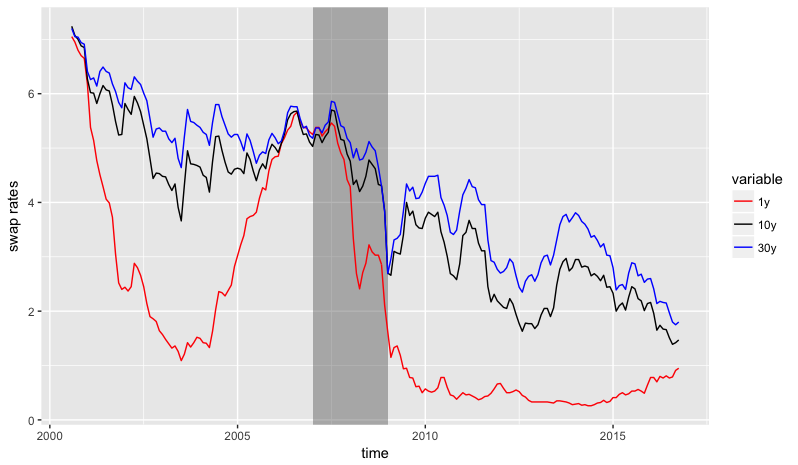
\includegraphics[width=14cm]{gfx/chapter-rvfl-mts/fredswaprates}
% figure caption is below the figure
\caption{Swap rates data (in \%) from St Louis Federal Reserve Bank, at maturities $1, 10, 30$}
\label{example3:1}       % Give a unique label
\end{figure}

\medskip

We also observe that the spreads between swap rates with different maturities start to narrow in 2006 until the end of 2007, and the  swap rates for short term maturities are relatively high during the same period. This is the period corresponding to the Liquidity and Credit Crunch 2007-2008. Table \ref{tab:freddatatables1} presents the descriptive statistics for these three time series.

\begin{table}
\begin{center}
% table caption is above the table
\caption{Descriptive statistics of St Louis Federal Reserve data for 1y, 10y and 30y swap rates (in \%)}
\label{tab:freddatatables1}       % Give a unique label
% For LaTeX tables use
\begin{tabular}{lllllll}
\hline\noalign{\smallskip}
Maturity & Min. & 1st Qrt & Median & Mean & 3rd Qrt & Max.\\
\noalign{\smallskip}\hline\noalign{\smallskip}
  1  & 0.260 & 0.500  & 1.340  & 2.108  & 3.360  & 7.050\\
  10 & 1.390 & 2.610  & 4.190  & 3.881  & 5.020  & 7.240\\
  30 & 1.750 & 3.270  & 4.650  & 4.404  & 5.375  & 7.200\\
\noalign{\smallskip}\hline
\end{tabular}
\end{center}
\end{table}

\medskip

All the swap rates (for all the maturities available) were then transformed into zero rates, by using a single curve calibration methodology (that is, ignoring the counterparty credit risk) with linear interpolation between the swaps' maturities. Then, the Nelson \& Siegel model was used for fitting and forecasting the curves in a DNS framework, with both \code{auto.arima} and the RVFL model presented in this chapter, applied to the three factors. In the fashion of section ~\ref{section:dnsexample1}. But now, we obtain 36-months ahead forecasts, from a rolling training windows with a fixed 36 months length. The average out-of-sample $RMSE$ are then calculated for each method.

\medskip

The \textit{best} hyperparameters - associated with the lowest out-of-sample average $RMSE$ - for each model are obtained through a search on a grid of values. We have:
\begin{itemize}
\item DNS with ARIMA (\code{auto.arima}): $\lambda = 1.4271$ (Nelson Siegel parameter)
\item DNS with RVFL: \textbf{number of lags} for each series: 1, \textbf{activation function}: ReLU, \textbf{number of nodes} in the hidden layer: $45$, $\lambda_1 = 4.6416$, $\lambda_2 = 774.2637$ (RVFL parameters) and $\lambda = 24$ (Nelson Siegel parameter)
\end{itemize}

\medskip

With these parameters, the results detailed in table \ref{tab:freddatatables4} are obtained, for the out-of-sample $RMSE$. A $95\%$ confidence interval around the difference of out-of-sample $RMSE$ between ARIMA (applied to each one of the three factors) and RVFL is presented in table \ref{tab:confint3}.

\begin{table}[!htb]
\begin{center}
% table caption is above the table
\caption{Descriptive statistics for out-of-sample $RMSE$, with rolling training window = 36 months, and testing window = 36 months}
\label{tab:freddatatables4}       % Give a unique label
% For LaTeX tables use
\begin{tabular}{llllllll}
\hline\noalign{\smallskip}
Method & Min. & 1st Qrt & Median & Mean & 3rd Qrt & Max. & Std. Dev\\
\noalign{\smallskip}\hline\noalign{\smallskip}
  ARIMA   & 0.0036  & \textbf{0.0070}  & \textbf{0.0104}  & 0.0149  & 0.0161  & 0.2150 & 0.0213\\
  RVFL    & \textbf{0.0032}  & 0.0078  & 0.0115  & \textbf{0.0120}  & \textbf{0.0148}  & \textbf{0.0256} & \textbf{0.0055}\\
\noalign{\smallskip}\hline
\end{tabular}
\end{center}
\end{table}

\begin{table}[!htb]
\begin{center}
% table caption is above the table
\caption{95\% confidence interval around the difference of out-of-sample $RMSE$}
\label{tab:confint3}       % Give a unique label
% For LaTeX tables use
\begin{tabular}{lllllll}
\hline\noalign{\smallskip}
Method & Lower bound & Upper bound  & Mean \\
\noalign{\smallskip}\hline\noalign{\smallskip}
  RVFL-ARIMA & -0.0064 & 0.0007 & \textbf{-0.0028} \\
\noalign{\smallskip}\hline
\end{tabular}
\end{center}
\end{table}

Figure \ref{example3:2} presents the evolution of the out-of-sample $log(RMSE)$ over the training/testing windows. The grey rectangle indicating the Liquidity and Credit crunch is larger here, because in this example, a training set starting in 2004 has its test set starting 36 months later, in 2007. Again, we observe that the results from the RVFL model exhibit a low out-of-sample error, along with a low volatility.

\begin{figure}[!htb]
\centering
% Use the relevant command to insert your figure file.
% For example, with the graphicx package use
  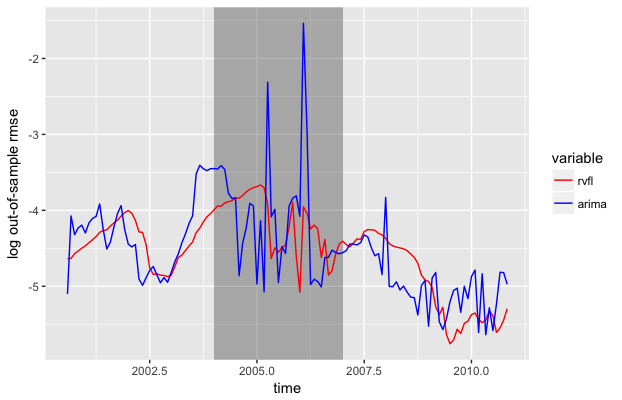
\includegraphics[width=14cm]{gfx/chapter-rvfl-mts/log_oos_rmse_rvfl_arima}
% figure caption is below the figure
\caption{Out-of-sample $log(RMSE)$, for ARIMA and RVFL over time}
\label{example3:2}       % Give a unique label
\end{figure}

\medskip

Figure \ref{example3:3}, presents the convergence of the out-of-sample $log(RMSE)$ for the DNS + RVFL model from this section, as a function of $log(\lambda_1)$ and $log(\lambda_2)$. $\lambda_1$ and $\lambda_2$ both range from $10^{-2}$ to $10^{4}$, with ten equally-spaced points each (hence, a grid of one hundred points $\left( log(\lambda_1), log(\lambda_2), log(RMSE)\right)$.

\medskip

The number of nodes in the hidden layer is equal to $45$, and the value of $\lambda$, parameter from the \cite{nelson1987parsimonious} model presented in section \ref{section:dnsexample1}, is fixed and equal to $24$. The one hundred points $\left( log(\lambda_1), log(\lambda_2), log(RMSE)\right)$ that we use for figure \ref{example3:3} can be found in appendix \ref{sec:cv_log_rmse}.

\medskip

There is a rectangular region at the top, in the middle of the figure, where the $log(RMSE)$ is the lowest. In this region, the lowest value of the out-of-sample $log(RMSE)$ is observed for $\lambda_1 = 4.6416$ and $\lambda_2 = 464.1589$ and the out-of-sample $RMSE$ is equal to $0.01206$ ($75^{th}$ point in appendix \ref{sec:cv_log_rmse}).

\begin{figure}[!htb]
\centering
% Use the relevant command to insert your figure file.
% For example, with the graphicx package use
  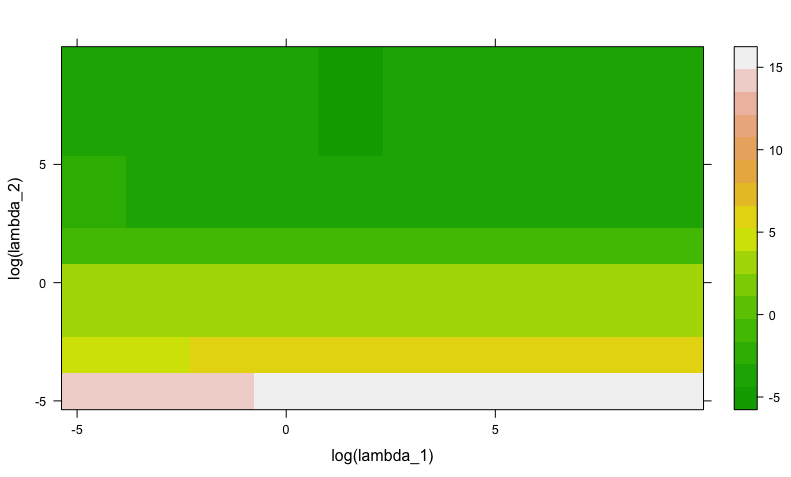
\includegraphics[width=14cm]{gfx/chapter-rvfl-mts/log_rmse_convergence}
% figure caption is below the figure
\caption{Out-of-sample $log(RMSE)$, as a function of $\lambda_1$ and $\lambda_2$}
\label{example3:3}       % Give a unique label
\end{figure}

\newpage

\section{Conclusion}

We present a model which could be used for multiple time series forecasting, based on a single layer quasi-randomized neural network. In this model, the lags of the different time series are used as in a dynamic regression model, and include the response variable lags. An additional layer of variables is added to the regression, whose nodes are not trained but obtained from a low discrepancy sequence. It is possible to add new variables to the regression, as indicators of special events, or to stress one variable, and observe the implied effect on the others' forecast. The model is tested on raw historical spot rates, and in a Dynamic Nelson Siegel framework. It produces \textit{robust} forecast results when compared to other usual (unpenalized) models in the same framework.

\newpage

\section{Appendix}

\subsection{Mean forecast and confidence intervals for $\alpha_{i, t}, i = 1, \ldots, 3$ forecasts}
\label{fcst_ci}

$\alpha_{1, t}$:

\begin{verbatim}
alpha1    y_lo80    y_hi80    y_lo95    y_hi95
13 0.7432724 0.6852024 0.8013425 0.6544620 0.8320829
14 0.7357374 0.6776673 0.7938074 0.6469269 0.8245478
15 0.7378042 0.6797342 0.7958742 0.6489938 0.8266147
16 0.7408417 0.6827717 0.7989118 0.6520313 0.8296522
17 0.7407904 0.6827204 0.7988604 0.6519800 0.8296009
18 0.7404501 0.6823801 0.7985201 0.6516396 0.8292605
19 0.7403603 0.6822903 0.7984303 0.6515498 0.8291707
20 0.7403981 0.6823281 0.7984681 0.6515876 0.8292085
21 0.7404788 0.6824087 0.7985488 0.6516683 0.8292892
22 0.7404786 0.6824086 0.7985487 0.6516682 0.8292891
23 0.7404791 0.6824091 0.7985491 0.6516686 0.8292895
24 0.7404758 0.6824058 0.7985458 0.6516654 0.8292863
\end{verbatim}

$\alpha_{2, t}$:

\begin{verbatim}
 alpha2    y_lo80    y_hi80    y_lo95    y_hi95
13 -1.250640 -1.351785 -1.149495 -1.405328 -1.095952
14 -1.243294 -1.344439 -1.142149 -1.397982 -1.088606
15 -1.241429 -1.342574 -1.140284 -1.396117 -1.086741
16 -1.243868 -1.345014 -1.142723 -1.398557 -1.089180
17 -1.244483 -1.345628 -1.143338 -1.399171 -1.089795
18 -1.241865 -1.343010 -1.140719 -1.396553 -1.087177
19 -1.240814 -1.341959 -1.139669 -1.395502 -1.086126
20 -1.240371 -1.341516 -1.139226 -1.395059 -1.085683
21 -1.240237 -1.341382 -1.139092 -1.394925 -1.085549
22 -1.240276 -1.341421 -1.139131 -1.394964 -1.085588
23 -1.240329 -1.341474 -1.139184 -1.395017 -1.085641
24 -1.240308 -1.341453 -1.139163 -1.394996 -1.085620
\end{verbatim}

$\alpha_{3, t}$:

\begin{verbatim}
 alpha3   y_lo80   y_hi80   y_lo95   y_hi95
13 4.584836 4.328843 4.757406 4.215410 4.870840
14 4.546167 4.307253 4.849862 4.163634 4.993482
15 4.527651 4.201991 4.803004 4.042913 4.962082
16 4.513810 4.216525 4.850160 4.048812 5.017874
17 4.517643 4.176214 4.828735 4.003502 5.001446
18 4.523109 4.203064 4.866713 4.027406 5.042371
19 4.522772 4.178489 4.848760 4.001079 5.026170
20 4.521846 4.191833 4.866066 4.013374 5.044524
21 4.521382 4.177560 4.854171 3.998472 5.033259
22 4.521451 4.186714 4.864755 4.007248 5.044222
23 4.521772 4.178995 4.857897 3.999300 5.037591
24 4.521862 4.184734 4.864155 4.004903 5.043987
\end{verbatim}

\subsection{Stressed forecast ($\alpha_{1, t} + 0.5\%$) and confidence intervals for $\alpha_{i, t}, i = 1, \ldots, 3$ forecasts}

$\alpha_{1, t}$:

\begin{verbatim}
 alpha1  y_lo80  y_hi80  y_lo95  y_hi95
13   1.25 1.19193 1.30807 1.16119 1.33881
14   1.25 1.19193 1.30807 1.16119 1.33881
15   1.25 1.19193 1.30807 1.16119 1.33881
16   1.25 1.19193 1.30807 1.16119 1.33881
17   1.25 1.19193 1.30807 1.16119 1.33881
18   1.25 1.19193 1.30807 1.16119 1.33881
19   1.25 1.19193 1.30807 1.16119 1.33881
20   1.25 1.19193 1.30807 1.16119 1.33881
21   1.25 1.19193 1.30807 1.16119 1.33881
22   1.25 1.19193 1.30807 1.16119 1.33881
23   1.25 1.19193 1.30807 1.16119 1.33881
24   1.25 1.19193 1.30807 1.16119 1.33881
\end{verbatim}

$\alpha_{2, t}$:

\begin{verbatim}
 alpha2    y_lo80    y_hi80    y_lo95    y_hi95
13 -1.222568 -1.323713 -1.121423 -1.377256 -1.067880
14 -1.219401 -1.320546 -1.118256 -1.374089 -1.064713
15 -1.211361 -1.312506 -1.110216 -1.366049 -1.056673
16 -1.216213 -1.317358 -1.115068 -1.370901 -1.061525
17 -1.215266 -1.316411 -1.114121 -1.369954 -1.060578
18 -1.211474 -1.312619 -1.110329 -1.366162 -1.056786
19 -1.210329 -1.311474 -1.109183 -1.365017 -1.055640
20 -1.209610 -1.310755 -1.108465 -1.364298 -1.054922
21 -1.209648 -1.310793 -1.108503 -1.364336 -1.054960
22 -1.209601 -1.310746 -1.108456 -1.364289 -1.054913
23 -1.209688 -1.310833 -1.108542 -1.364376 -1.055000
24 -1.209653 -1.310798 -1.108508 -1.364341 -1.054965
\end{verbatim}

$\alpha_{3, t}$:

\begin{verbatim}
alpha3   y_lo80   y_hi80   y_lo95   y_hi95
13 4.500390 4.244398 4.672961 4.130964 4.786394
14 4.482948 4.244035 4.786643 4.100415 4.930263
15 4.441841 4.116182 4.717194 3.957103 4.876272
16 4.441744 4.144459 4.778094 3.976746 4.945808
17 4.439609 4.098181 4.750701 3.925469 4.923413
18 4.447151 4.127105 4.790755 3.951448 4.966412
19 4.446164 4.101881 4.772152 3.924471 4.949562
20 4.445421 4.115407 4.789641 3.936949 4.968099
21 4.445411 4.101589 4.778200 3.922501 4.957289
22 4.445491 4.110754 4.788795 3.931287 4.968262
23 4.445937 4.103160 4.782062 3.923465 4.961756
24 4.446012 4.108885 4.788306 3.929053 4.968137
\end{verbatim}

\newpage

\nocite{dutang2015}
\nocite{wickham2016ggplot2}


\section{Appendix}

\subsection{Mean forecast and confidence intervals for $\alpha_{i, t}, i = 1, \ldots, 3$ forecasts}

$\alpha_{1, t}$:

\begin{verbatim}
alpha1    y_lo80    y_hi80    y_lo95    y_hi95
13 0.7432724 0.6852024 0.8013425 0.6544620 0.8320829
14 0.7357374 0.6776673 0.7938074 0.6469269 0.8245478
15 0.7378042 0.6797342 0.7958742 0.6489938 0.8266147
16 0.7408417 0.6827717 0.7989118 0.6520313 0.8296522
17 0.7407904 0.6827204 0.7988604 0.6519800 0.8296009
18 0.7404501 0.6823801 0.7985201 0.6516396 0.8292605
19 0.7403603 0.6822903 0.7984303 0.6515498 0.8291707
20 0.7403981 0.6823281 0.7984681 0.6515876 0.8292085
21 0.7404788 0.6824087 0.7985488 0.6516683 0.8292892
22 0.7404786 0.6824086 0.7985487 0.6516682 0.8292891
23 0.7404791 0.6824091 0.7985491 0.6516686 0.8292895
24 0.7404758 0.6824058 0.7985458 0.6516654 0.8292863
\end{verbatim}

$\alpha_{2, t}$:

\begin{verbatim}
 alpha2    y_lo80    y_hi80    y_lo95    y_hi95
13 -1.250640 -1.351785 -1.149495 -1.405328 -1.095952
14 -1.243294 -1.344439 -1.142149 -1.397982 -1.088606
15 -1.241429 -1.342574 -1.140284 -1.396117 -1.086741
16 -1.243868 -1.345014 -1.142723 -1.398557 -1.089180
17 -1.244483 -1.345628 -1.143338 -1.399171 -1.089795
18 -1.241865 -1.343010 -1.140719 -1.396553 -1.087177
19 -1.240814 -1.341959 -1.139669 -1.395502 -1.086126
20 -1.240371 -1.341516 -1.139226 -1.395059 -1.085683
21 -1.240237 -1.341382 -1.139092 -1.394925 -1.085549
22 -1.240276 -1.341421 -1.139131 -1.394964 -1.085588
23 -1.240329 -1.341474 -1.139184 -1.395017 -1.085641
24 -1.240308 -1.341453 -1.139163 -1.394996 -1.085620
\end{verbatim}

$\alpha_{3, t}$:

\begin{verbatim}
 alpha3   y_lo80   y_hi80   y_lo95   y_hi95
13 4.584836 4.328843 4.757406 4.215410 4.870840
14 4.546167 4.307253 4.849862 4.163634 4.993482
15 4.527651 4.201991 4.803004 4.042913 4.962082
16 4.513810 4.216525 4.850160 4.048812 5.017874
17 4.517643 4.176214 4.828735 4.003502 5.001446
18 4.523109 4.203064 4.866713 4.027406 5.042371
19 4.522772 4.178489 4.848760 4.001079 5.026170
20 4.521846 4.191833 4.866066 4.013374 5.044524
21 4.521382 4.177560 4.854171 3.998472 5.033259
22 4.521451 4.186714 4.864755 4.007248 5.044222
23 4.521772 4.178995 4.857897 3.999300 5.037591
24 4.521862 4.184734 4.864155 4.004903 5.043987
\end{verbatim}

\subsection{Stressed forecast ($\alpha_{1, t} + 0.5\%$) and confidence intervals for $\alpha_{i, t}, i = 1, \ldots, 3$ forecasts}

$\alpha_{1, t}$:

\begin{verbatim}
 alpha1  y_lo80  y_hi80  y_lo95  y_hi95
13   1.25 1.19193 1.30807 1.16119 1.33881
14   1.25 1.19193 1.30807 1.16119 1.33881
15   1.25 1.19193 1.30807 1.16119 1.33881
16   1.25 1.19193 1.30807 1.16119 1.33881
17   1.25 1.19193 1.30807 1.16119 1.33881
18   1.25 1.19193 1.30807 1.16119 1.33881
19   1.25 1.19193 1.30807 1.16119 1.33881
20   1.25 1.19193 1.30807 1.16119 1.33881
21   1.25 1.19193 1.30807 1.16119 1.33881
22   1.25 1.19193 1.30807 1.16119 1.33881
23   1.25 1.19193 1.30807 1.16119 1.33881
24   1.25 1.19193 1.30807 1.16119 1.33881
\end{verbatim}

$\alpha_{2, t}$:

\begin{verbatim}
 alpha2    y_lo80    y_hi80    y_lo95    y_hi95
13 -1.222568 -1.323713 -1.121423 -1.377256 -1.067880
14 -1.219401 -1.320546 -1.118256 -1.374089 -1.064713
15 -1.211361 -1.312506 -1.110216 -1.366049 -1.056673
16 -1.216213 -1.317358 -1.115068 -1.370901 -1.061525
17 -1.215266 -1.316411 -1.114121 -1.369954 -1.060578
18 -1.211474 -1.312619 -1.110329 -1.366162 -1.056786
19 -1.210329 -1.311474 -1.109183 -1.365017 -1.055640
20 -1.209610 -1.310755 -1.108465 -1.364298 -1.054922
21 -1.209648 -1.310793 -1.108503 -1.364336 -1.054960
22 -1.209601 -1.310746 -1.108456 -1.364289 -1.054913
23 -1.209688 -1.310833 -1.108542 -1.364376 -1.055000
24 -1.209653 -1.310798 -1.108508 -1.364341 -1.054965
\end{verbatim}

$\alpha_{3, t}$:

\begin{verbatim}
alpha3   y_lo80   y_hi80   y_lo95   y_hi95
13 4.500390 4.244398 4.672961 4.130964 4.786394
14 4.482948 4.244035 4.786643 4.100415 4.930263
15 4.441841 4.116182 4.717194 3.957103 4.876272
16 4.441744 4.144459 4.778094 3.976746 4.945808
17 4.439609 4.098181 4.750701 3.925469 4.923413
18 4.447151 4.127105 4.790755 3.951448 4.966412
19 4.446164 4.101881 4.772152 3.924471 4.949562
20 4.445421 4.115407 4.789641 3.936949 4.968099
21 4.445411 4.101589 4.778200 3.922501 4.957289
22 4.445491 4.110754 4.788795 3.931287 4.968262
23 4.445937 4.103160 4.782062 3.923465 4.961756
24 4.446012 4.108885 4.788306 3.929053 4.968137
\end{verbatim}

\subsection{Out-of-sample $log(RMSE)$ as a function of $log(\lambda_1)$ and $log(\lambda_2)$}
\label{sec:cv_log_rmse}

\begin{verbatim}
    log_lambda1 log_lambda2  log_error
1     -4.605170   -4.605170 13.5039336
2     -3.070113   -4.605170 14.3538621
3     -1.535057   -4.605170 14.7912525
4      0.000000   -4.605170 14.8749375
5      1.535057   -4.605170 14.8928025
6      3.070113   -4.605170 14.8962203
7      4.605170   -4.605170 14.8975776
8      6.140227   -4.605170 14.8976494
9      7.675284   -4.605170 14.8976630
10     9.210340   -4.605170 14.8976715
11    -4.605170   -3.070113  3.9701229
12    -3.070113   -3.070113  4.9644144
13    -1.535057   -3.070113  5.2607788
14     0.000000   -3.070113  5.3208833
15     1.535057   -3.070113  5.3326856
16     3.070113   -3.070113  5.3351784
17     4.605170   -3.070113  5.3357136
18     6.140227   -3.070113  5.3358306
19     7.675284   -3.070113  5.3358557
20     9.210340   -3.070113  5.3358610
21    -4.605170   -1.535057  3.6692928
22    -3.070113   -1.535057  3.5643607
23    -1.535057   -1.535057  3.5063072
24     0.000000   -1.535057  3.4942438
25     1.535057   -1.535057  3.4904354
26     3.070113   -1.535057  3.4881352
27     4.605170   -1.535057  3.4888202
28     6.140227   -1.535057  3.4880668
29     7.675284   -1.535057  3.4886911
30     9.210340   -1.535057  3.4886383
31    -4.605170    0.000000  3.6224691
32    -3.070113    0.000000  3.8313407
33    -1.535057    0.000000  3.8518759
34     0.000000    0.000000  3.8163287
35     1.535057    0.000000  3.7993471
36     3.070113    0.000000  3.7948073
37     4.605170    0.000000  3.7937787
38     6.140227    0.000000  3.7935546
39     7.675284    0.000000  3.7935063
40     9.210340    0.000000  3.7934958
41    -4.605170    1.535057 -1.2115597
42    -3.070113    1.535057 -1.0130537
43    -1.535057    1.535057 -0.5841784
44     0.000000    1.535057 -0.3802817
45     1.535057    1.535057 -0.3109827
46     3.070113    1.535057 -0.2931830
47     4.605170    1.535057 -0.2891586
48     6.140227    1.535057 -0.2882824
49     7.675284    1.535057 -0.2880932
50     9.210340    1.535057 -0.2880524
51    -4.605170    3.070113 -2.0397856
52    -3.070113    3.070113 -3.1729003
53    -1.535057    3.070113 -3.8655596
54     0.000000    3.070113 -3.9279840
55     1.535057    3.070113 -3.9508440
56     3.070113    3.070113 -4.0270316
57     4.605170    3.070113 -4.0831569
58     6.140227    3.070113 -4.0953167
59     7.675284    3.070113 -4.0979447
60     9.210340    3.070113 -4.0985113
61    -4.605170    4.605170 -2.6779260
62    -3.070113    4.605170 -3.4704808
63    -1.535057    4.605170 -4.0404935
64     0.000000    4.605170 -4.2441836
65     1.535057    4.605170 -4.3657802
66     3.070113    4.605170 -4.3923094
67     4.605170    4.605170 -4.3862826
68     6.140227    4.605170 -4.3830293
69     7.675284    4.605170 -4.3820703
70     9.210340    4.605170 -4.3818486
71    -4.605170    6.140227 -3.5007058
72    -3.070113    6.140227 -3.8389274
73    -1.535057    6.140227 -4.1969545
74     0.000000    6.140227 -4.3400025
75     1.535057    6.140227 -4.4179718
76     3.070113    6.140227 -4.3797034
77     4.605170    6.140227 -4.3073100
78     6.140227    6.140227 -4.2866647
79     7.675284    6.140227 -4.2820357
80     9.210340    6.140227 -4.2810151
81    -4.605170    7.675284 -3.7236774
82    -3.070113    7.675284 -4.0057353
83    -1.535057    7.675284 -4.2699684
84     0.000000    7.675284 -4.3569254
85     1.535057    7.675284 -4.4156364
86     3.070113    7.675284 -4.3842360
87     4.605170    7.675284 -4.2759516
88     6.140227    7.675284 -4.2425876
89     7.675284    7.675284 -4.2346514
90     9.210340    7.675284 -4.2328863
91    -4.605170    9.210340 -3.7706268
92    -3.070113    9.210340 -4.0406387
93    -1.535057    9.210340 -4.2776907
94     0.000000    9.210340 -4.3498230
95     1.535057    9.210340 -4.4095778
96     3.070113    9.210340 -4.3860089
97     4.605170    9.210340 -4.2647179
98     6.140227    9.210340 -4.2273624
99     7.675284    9.210340 -4.2183911
100    9.210340    9.210340 -4.2163638
\end{verbatim}

 % INCLUDE: rvfl-mts
\forcenewpage

%\forcenewpage

%% !TEX root = ../thesis-example.tex
%
\chapter{Conclusion}
\label{sec:conclusion}

 % INCLUDE: conclusion
%\cleardoublepage
=======
% !TEX root = ../thesis-example.tex
%
\chapter{Multiple time series forecasting using ensembles of quasi-randomized functional link neural networks}
\label{sec:rvfl_ensembles}

\section{Introduction}

The goal of ensemble learning is to combine two or more individual statistical/machine learning models - the base models or base learners - into one, in order to obtain an ensemble model, with an improved out-of-sample error over the base models.

\medskip

Ensemble learning is widely used in the winning solutions of machine learning competitions. It allows to achieve very good performances indeed, at the expense of being relatively less interpretable than the base learners. As a consequence, choosing to use ensemble models or a base model for solving a given problem, could sometimes be seen as finding a trade-off between the desire for interpretability and the desire for an highly increased performance. That said, some techniques such as variable importance for ensemble of trees, can give a sense of which predictor contributes the most to the perfomance of the model.

\medskip

In this chapter, we apply three popular ensemble learning methods to multiple time series forecasting: Bootstrap aggregating (\cite{breiman1996bagging}), known as bagging, Boosting (\cite{friedman2001greedy}, \cite{buhlmann2003boosting}, \cite{hothorn2010model}), and stacked generalization(\cite{wolpert1992stacked}), known as stacking. The base learners that we use for bagging and stacking, are the quasi-random vector functional link neural networks introduced in \cite{moudiki2018multiple}. For the boosting algorithm, we use a slightly modified version of the model from \cite{moudiki2018multiple}, in which the regression model parameters are not constrained in a ridge regression fashion (more details in section \ref{sec:basemodeldesc}).  

\medskip

In the next section, we give an overview of the base learners. Then, we describe how we use these models as the basic components of our bagged/stacked ensembles. To finish, we present some numerical examples of use of these new models for forecasting multiple time series.

\section{Description of the base models}
\label{sec:basemodeldesc}

The base learner is described in lengths in \cite{moudiki2018multiple}. It is a single layer feed forward neural networks (SLFN). We have an output variable $y \in \RR^n$, which has to be explained by a set of observed predictors $X^{(j)} \in \RR^n$, $j \in \left\lbrace 1, \ldots,
p\right\rbrace$. The RVFL networks that we use to explain $y$ is described for $i \in \left\lbrace 1, \ldots, n\right\rbrace$ as:

\begin{equation}
\label{eq:rvflequation}
y_i = \beta_0 + \sum_{j = 1}^p \beta_j X_i^{(j)} + \sum_{l = 1}^L \gamma_l \:
g\left(\sum_{j = 1}^p W^{(j, l)} X_i^{(j)}\right) + \epsilon_i
\end{equation}

\medskip

Where $g$ is the \textit{activation function}, $L$ the number of nodes in the hidden
layer, $W^{(j, l)}$ are elements of the hidden layer, and the parameters
$\beta_j$ and $\gamma_l$ are to be learned from the observed data $X^{(j)}, \: j
\in \left\lbrace 1, \ldots, p\right\rbrace$. The $\epsilon_i$'s are the residual
differences between the output variable values and the RVFL model.

\medskip

This type of model can be seen as a one explaining $y_i$, by finding a
compromise between linear and potentially non-linear effects of the original
predictors $X^{(j)}$ and transformed predictors
$$
\Phi(\bfX)^{(l)}= g\left(\sum_{j = 1}^p W^{(j, l)} X_i^{(j)}\right)
$$
$\left \lbrace 1, \ldots, L\right\rbrace$ on the response. In this paper, we use the Rectified Linear Units activation function, known as ReLU
$$
g: \: x \mapsto max(x, 0)
$$
But other choices of activation functions, such as the sigmoid function $g: \: x \mapsto \frac{1}{1+exp(-x)}$ or the hyperbolic tangent $g: \: x \mapsto tanh(x)$ (or others) can be envisaged.

\medskip

The elements $W^{(j, l)}$ of the hidden layer are taken from a quasi-random (deterministic) \textit{sobol} sequence on $[0, 1]$, which is shifted in such a way that they belong to $[-1, 1]$. In the case of bagged and stacked ensembles, solving for the optimal $\beta_j$'s and $\gamma_l$'s in the base-learners is done by searching these parameters,  in restricted regions where we have:
$$
\sum_{j=1}^p \beta_j^2  \leq u
$$
and
$$
\sum_{l=1}^L
\gamma_l^2 \leq v
$$ for $u, v \in \RR^*$. That is, by applying a regularization to these unknown parameters. In the case of boosting, we do not restrict the regression parameters' norms to be inferior to $u$ and $v$. Instead, we rely on the boosting algorithm described in \cite{hothorn2010model} (details in section \ref{sec:rvflboosting}), with the base-learners being the unrestricted regression models described by equation (\ref{eq:rvflequation}). 


\medskip

If we consider $p \in \mathbb{N}^*$ time series $(X_t^{(j)})_{t \geq 0}, j = 1, \ldots, p$, observed at $n \in \mathbb{N}^*$ discrete dates, we are interested in
obtaining simultaneous forecasts of the $p$ time series at time $n+h$, $h \in
\mathbb{N}^*$, by allowing each of the $p$ variables to be influenced by the
others. We use $k < n$ lags of each of the observed $p$ time
series. So that, the output variables to be explained are:

\begin{equation}
Y^{(j)} = \left(X^{(j)}_n, \ldots, X^{(j)}_{k+1} \right)^T
\end{equation}

for $j \in \left\lbrace 1, \ldots,
p \right\rbrace$. $X^{(j)}_n$ is the most contemporaneous observed value
of the $j^{th}$ time series, and $X^{(j)}_{k+1}$ was observed $k$ dates earlier
in time for $(X^{(j)}_t)_{t \geq 0}$. These output variables are stored in a
matrix: $$ \bfY \in \RR^{(n-k) \times p} $$ and the predictors are
stored in a matrix: $$ \bfX \in \RR^{(n-k) \times (k \times p)} $$
where $\bfX$ consists in $p$ blocks of $k$ lags, for each one of the observed
$p$ time series.

\medskip

An additional layer of transformed  predictors
is added to $\bfX$, in order to capture the potentially non-linear
interactions between the predictors and the output variable. This also serve as a way to do achieve an automated feature engineering. Adding the transformed predictors to the original ones, leads to a new matrix of predictors with dimensions $(n-k) \times (k \times p + L)$, where $L$ is the number of nodes in the hidden layer.

\medskip

For example, we have $p = 2$ time series $(X^{(1)}_{t_1}, \ldots,  X^{(1)}_{t_5})$ and $(X^{(2)}_{t_1}, \ldots,  X^{(2)}_{t_5})$ observed at $n = 5$ dates, $t_1 < \ldots < t_5$, with $k = 2$ lags, and $L = 3$ nodes in the hidden layer. In this case, the response variables are stored in:
$$
\bfY = \left( {\begin{array}{cc} X^{(1)}_{t_5} &  X^{(2)}_{t_5}\\ X^{(1)}_{t_4} & X^{(2)}_{t_4} \\ X^{(1)}_{t_3} & X^{(2)}_{t_3}\      \end{array} } \right)
$$
The predictors are stored in:
$$
\bfX = \left( {\begin{array}{cccc} X^{(1)}_{t_4} & X^{(1)}_{t_3} & X^{(2)}_{t_4} & X^{(2)}_{t_3} \\ X^{(1)}_{t_3} & X^{(1)}_{t_2} & X^{(2)}_{t_3} & X^{(2)}_{t_2} \\ X^{(1)}_{t_2} & X^{(1)}_{t_1} & X^{(2)}_{t_2} & X^{(2)}_{t_1} \      \end{array} }\right)
$$
And the coefficients in the hidden layer are:
$$
\textbf{W} = \left( {\begin{array}{ccc} W^{(1, 1)} & W^{(1, 2)} & W^{(1, 3)}  \\ W^{(2, 1)} & W^{(2, 2)} & W^{(2, 3)}  \\ W^{(3, 1)} & W^{(3, 2)} & W^{(3, 3)} \\ W^{(4, 1)} & W^{(4, 2)} & W^{(4, 3)}  \      \end{array} }\right)
$$

\medskip

We let $y$ be the $j_0^{th}$ column (out of $p$) of the response matrix $\bfY$, and $\Phi(\bfX)$ be the matrix of transformed predictors obtained from $\bfX$ by the hidden layer. We also denote the set of regression parameters associated with this $j_0^{th}$ time series, as:
$$
\beta_m^{(j_0)} =: \beta_m
$$
and
$$
\gamma_l^{(j_0)} =: \gamma_l
$$

for $m \in \left\lbrace 1, \ldots, k \right\rbrace$; $l \in \left\lbrace 1, \ldots,  L\right\rbrace$. Solving for the regression parameters for the $j_0^{th}$ time series, under the constraints
$$
\sum_{m=1}^{k\times p} \beta_m^2 \leq u
$$
and
$$
\sum_{l=1}^L \gamma_l^2 \leq v
$$
for $u, v \in \RR^*$, leads to minimizing a penalized residual sum of squares:
$$
\mathcal{L}(\bfX; \beta, \gamma) = \left(y - \bfX\beta -
\Phi(\bfX)\gamma\right)^T\left(y - \bfX\beta - \Phi(\bfX)\gamma\right) + \lambda_1
\beta^T \beta + \lambda_2 \gamma^T\gamma
$$

\medskip

where $\lambda_1$ and $\lambda_2$ are Lagrange multipliers. Otherwise, without the constraints (in the case of boosting, see section \ref{sec:rvflboosting}), the problem to be solved is simply a least squares regression problem on the augmented dataset, as described in equation \ref{sec:basemodeldesc}. By denoting:

$$ A = \left( {\begin{array}{cc} \bfX^T\bfX + \lambda_1 I_{k\times p} &  \bfX^T\Phi(\bfX)\\
\Phi(\bfX)^T\bfX & \Phi(\bfX)^T\Phi(\bfX) + \lambda_2 I_{L} \      \end{array} } \right) =:
\left( {\begin{array}{cc} B &  C^T\\ C & D \      \end{array} } \right) $$

and $S = D - CB^+C^T$. And:

$$
A^+ = \left( {\begin{array}{cc} B^+ + B^+ C^T
S^+ CB^+  &  -B^+ C^T S^+\\ -S^+CB^+ & S^+ \      \end{array} } \right) =:
\left( {\begin{array}{cc} A_1^+  &  A_2^+\\ A_3^+ & A_4^+ \      \end{array} }
\right)
$$


where $S^+$ and $B^+$ are the Moore-Penrose pseudo-inverse of matrices $S$ and
$B$. The whole set of parameters, for all the $p$ observed time series is given by:

$$
\left( {\begin{array}{c} \bm{\hat{\beta}} \\       \bm{\hat{\gamma}} \      \end{array}
} \right) := \left( {\begin{array}{cc} A_1^+  &  A_2^+\\ A_3^+ & A_4^+ \      \end{array}
} \right)\left( {\begin{array}{c} \bfX^T\bfY \\       \Phi(\bfX)^T\bfY \      \end{array} }
\right)
$$

\section{Ensembles of RVFL}
\label{sec:ensemblemethods}

As mentioned in the introduction, we will use bagging, boosting, and stacking to construct ensemble models, consisting of the RVFL models from the previous section \ref{sec:basemodeldesc}. A short description of these techniques will be made in next sections ~\ref{sec:rvflbagging}, ~\ref{sec:rvflboosting}  and \ref{sec:rvflstacking}.

\subsection{Bagging}
\label{sec:rvflbagging}

The Bootstrap (\cite{efron1986bootstrap}, \cite{efron1992bootstrap}) uses multiple random replications of a given data set, to obtain standard errors of model parameters, for example. In the context of ensemble learning, these replications of the original data set are used to produce various predictions of the base models, which are then aggregated - in the case of regression problems, they are averaged, and in the case of classification problems, majority vote could be used - to obtain a single prediction with less out-of-sample variance. This procedure is called bootstrap aggregating or \textit{bagging}.

\medskip

In order to illustrate the benefits of the bagging procedure, we consider $n$ different base learners, with out-of-sample prediction errors equal to $\epsilon_1, \ldots, \epsilon_n$, and assume that the distribution of these errors are centered around $0$:
$$
\EE \left[ \epsilon_i\right] = 0
$$
for $i = 1, \ldots, n$. In addition, we have:
$$
\EE \left[ \epsilon_i \epsilon_j\right] = \gamma
$$
for $i \neq j$; that is, the covariance between the errors is equal to $\gamma$. And:
$$
Var(\epsilon_i) = \sigma^2
$$
for $i = 1, \ldots, n$. The out-of-sample mean squared error (MSE) of the aggregated (averaged) model including these $n$ base models is equal to:

\begin{eqnarray*}
MSE = \EE\left[ \left( \frac{1}{n} \sum_{i = 1}^n \epsilon_i \right)^2 \right] &=& \frac{1}{n^2} \EE\left[ \left( \sum_{i = 1}^n \epsilon_i \right)^2 \right]\\
 &=& \frac{1}{n^2} \EE\left[ \sum_{i = 1}^n \epsilon_i^2 + 2 \sum_{i < j} \epsilon_i \epsilon_j  \right]\\
 &=& \frac{1}{n^2} \left( \sum_{i = 1}^n \EE\left[\epsilon_i^2\right] + 2 \sum_{i < j} \EE\left[\epsilon_i \epsilon_j  \right] \right)\\
 &=& \frac{1}{n^2} \left( n \sigma^2 + 2 \frac{n(n-1)}{2} \gamma \right)\\
 &=& \frac{\sigma^2}{n} + \frac{(n-1)}{n} \gamma \\
\end{eqnarray*}

From this expression of the $MSE$, we can observe that if $n$ is high ($n \rightarrow \infty$), that is, if there are several base learners in the ensemble, and the out-of-sample expected error is low, the out-of-sample MSE of the ensemble prediction will decrease, and can eventually be reduced to $\gamma$. If, in addition, the model predictions are perfectly uncorrelated, i.e $\gamma ~= 0$, then the out-of-sample MSE is further decreased.

\medskip

Having a low value for $\gamma$, along with a low out-of-sample expected error, helps in achieving a lower out-of-sample prediction error for the ensemble model. Decorrelation in ensemble learning is hence important, and consists in increasing the diversity in the base learners, in order to obtain a low value for $\gamma$.

\medskip

This decorrelation among the base learners is achieved for example in Random Forest models \cite{breiman2001random}, by growing each tree in the forest, with only a subset of the predictors available. Also, an example of use of decorrelation, specifically for ensembles of neural networks is demonstrated in \cite{rosen1996ensemble}. The author presents three approaches for achieving \textit{disagreement} between the networks: one in which they are trained independently and aggregated with the hope that their predictions are somewhat different; a second one, in which different activation functions or achitecture (typically, more or less hidden layers or nodes in the hidden layers etc.) for each base learner. A third approach consists in training the individual networks on different subsamples of the original training set. The case of decorrelation learning for RVFL is treated in \cite{alhamdoosh2014fast}.

\medskip

In both papers, \cite{rosen1996ensemble} and \cite{alhamdoosh2014fast}, the procedure implemented in order to obtain a decorrelation of the base learners is denoted as Negative Correlation Learning (NCL). The general idea is to minimize the penalized Root Mean Squared Error:
$$
\sum_{i = 1}^n\left[\left(y_i - f_k(\textbf{x}_i)\right)^2 + \lambda p_k(\textbf{x}_i)\right]
$$
where $\textbf{x}_i \in \RR^p$ is the $i^{th}$ observation of the training data set, with $p$ features. $f_k$ is a base learner with $k \in \left \lbrace 1 \ldots B\right \rbrace$, and $B$ is the number of bootstrap resamples. $p_k$ is a penalty term decorrelating the current network's error with the errors of the networks previously trained. $\lambda$ is a Lagrange multiplier, a regularization parameter, preventing the correlation between the successive base learners in-sample errors from being high. For example, $p_k$ could be defined as:
$$
p_k(\textbf{x}_i) = \left(y_i - f_k(\textbf{x}_i)\right)\sum_{j < k}\left(y_i - f_j(\textbf{x}_i)\right)
$$

\medskip

In this chapter, we use the third approach described in \cite{rosen1996ensemble}  (although many other approaches can be envisaged),  which is actually more \textit{subsampling} than bootstrapping. Multiple samples (training) data sets are constructed by randomly picking a fraction \code{col\underline{ }sample\underline{ }coeff} of the covariates, and a subset (using the fraction \code{row\underline{ }sample\underline{ }coeff}) of the lines, as described in figure \ref{bootstrap_resampling_plot} (using notations from section \ref{sec:basemodeldesc}). 

Taking a subset of the lines is done by respecting the serial dependence of the series and taking consecutive observations (that is, without skipping any observation) for each bootstrap resample. 

The predictions associated to each training set resample are then averaged, in order to obtain a single prediction, with an uncertainty around it. Some numerical examples on the application of bagging to RVFL base learners can be found in section \ref{sec:numericalexamples}

\begin{figure}[!htb]
\centering
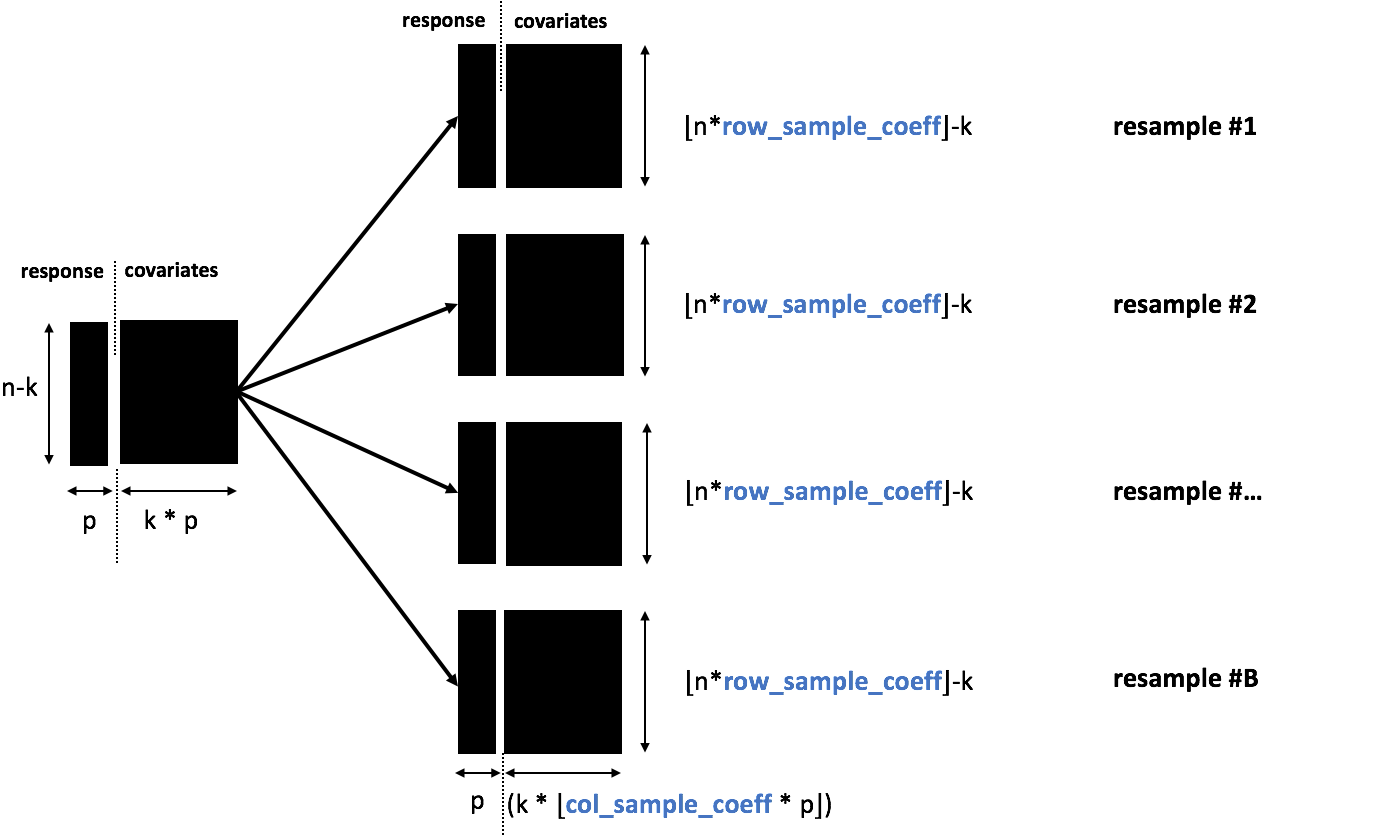
\includegraphics[width=10.5cm]{gfx/chapter-rvfl-ensembles/bootstrap_resampling.png}
\caption{Construction of $B$ bootstrap resamples by using the initial data}
\label{bootstrap_resampling_plot}
\end{figure}

\newpage

\subsection{Boosting}
\label{sec:rvflboosting}

The boosting approach adopted here, is described in \cite{hothorn2010model} and implemented in \proglang{R} package \code{mboost}. The general idea of the algorithm is to fit the in-sample residuals with base-learners, iteratively and slowly, but to stop learning before the out-of-sample error starts to worsen. With the response being $y$ and the covariates stored in  $\textbf{x}$, we are interested in constructing a regression function $\hat{f}$, so that: 
$$
\hat{f}(\textbf{x}) = \sum_{j=1}^B \nu \hat{f}_j(\textbf{x}) 
$$
$B$ is the number of boosting iterations, $\nu$ is a learning rate parameter preventing the base learners from fitting the residuals too quickly, and  $\hat{f}_j$, $j \in \left \lbrace 1, \ldots, B \right \rbrace$ are the base learners, which are obtained as: 
$$
\left(\hat{f}_1, \ldots,  \hat{f}_p\right) = argmin_{f_1, \ldots, f_p}  \rho \left( y, \sum_j \nu f_j\left( \textbf{x} \right) \right) 
$$

In this expression, $\rho$ is a loss function to be minimized (for example $x \mapsto x^2$, or $x \mapsto |x|$). And in the case of multivariate time series, we are doing multitask learning. Each series (their most contemporaneous observations) share the same set of predictors (their lagged observations) as in the RVFL model described in section \ref{sec:basemodeldesc}, but without regularization of the regression models' parameters. 

The same number of boosting iterations and the same learning rate are used for all the observed time series. It would be possible to consider different numbers of iterations and different learning rates for each time series, but in this situation there would be as much as parameters as time series, and the regularization parameters would be trickier to optimize. 

\subsection{Stacking}
\label{sec:rvflstacking}

Stacked generalization or stacking, was introduced in \cite{wolpert1992stacked}. It is also presented in \cite{breiman1996stacked} for regression models. The idea behind this procedure is to construct new predictors for the training data set, by using diverse predictions of multiple models, which are combined by a meta-learner model. A simple example of 2-fold stacking applied to regression is described hereafter. It is possible to imagine examples with more stacked layers:

\begin{itemize}
\item Divide the original training data set $\textbf{X} \in \RR^{n \times p}$, into two parts: \code{part1} and \code{part2}, each with $n/2$ rows
\item Train a base learner model on \code{part1} and obtain $n/2$ predictions on \code{part2}.
\item Train the same base learner model on \code{part2} and obtain $n/2$ predictions on \code{part1}.
\item Train a  meta-learner model on the new data set \code{part3}, consisting in the the original predictors, plus the predictors constructed by applying the base learner model on \code{part1} and \code{part2}.
\end{itemize}
\medskip

Typically, in this procedure, various types of base learners are used, to increate the diversity of new predictors. Since we are using time series data here, which inherently exhibit a serial dependence between the observations, we have to adapt the procedure described previously. In the case of a 2-fold stacking again, we divide the original training data set  $\textbf{X} \in \RR^{n \times p}$ (with $p$ time series observed at $n$ dates) into two parts: \code{part1} and \code{part2}; each consisting of $n/2$ rows. \code{part1} contains the most ancient observations and \code{part2}, the most recent observations of the time series contained in $\textbf{X}$. Also, we use multiple resamples of the base learner, as follows (this procedure is also described in figure \ref{rvfl_stacking_plot}):

\begin{itemize}
\item Train $B$ resampled RVFL models on \code{part1}, using a random subset of \code{part1} in each resampling iteration. Obtain $B$ sets of predictions ($B \times p$ new predictors) with these models, over the whole horizon  of \code{part2}.
\item Create a new enriched data set \code{part3}, containing the observed time series from \code{part2}, and the $B \times p$ additional series predicted from \code{part1} on \code{part2}.
\item Use a meta-learning model to obtain predictions on the new, enriched dataset, \code{part3}.
\end{itemize}

For the latter point, we consider a few meta-learner models that have been used in the past in the literature (\cite{breiman1996stacked}). In general, the idea is that a relatively simple meta-learner will achieve a good performance. We use the following models for this purpose:
\begin{itemize}
\item Linear \textbf{least squares regression} model.
\item Linear least squares regression model \textbf{with positive coefficients} (\cite{lawson1974solving}, \cite{lawson1995solving}), as used in \cite{breiman1996stacked}.
\item \textbf{Ridge regression} (\cite{hoerl1970ridge}).
\end{itemize}

These selected meta-learners are trained on \code{part3}, with the most contemporaneous observations of the series as responses, and their respective lags as predictors. Some numerical examples on the application of stacking to RVFL base learners can be found in section \ref{sec:numericalexamples}

\begin{figure}[!htb]
\centering
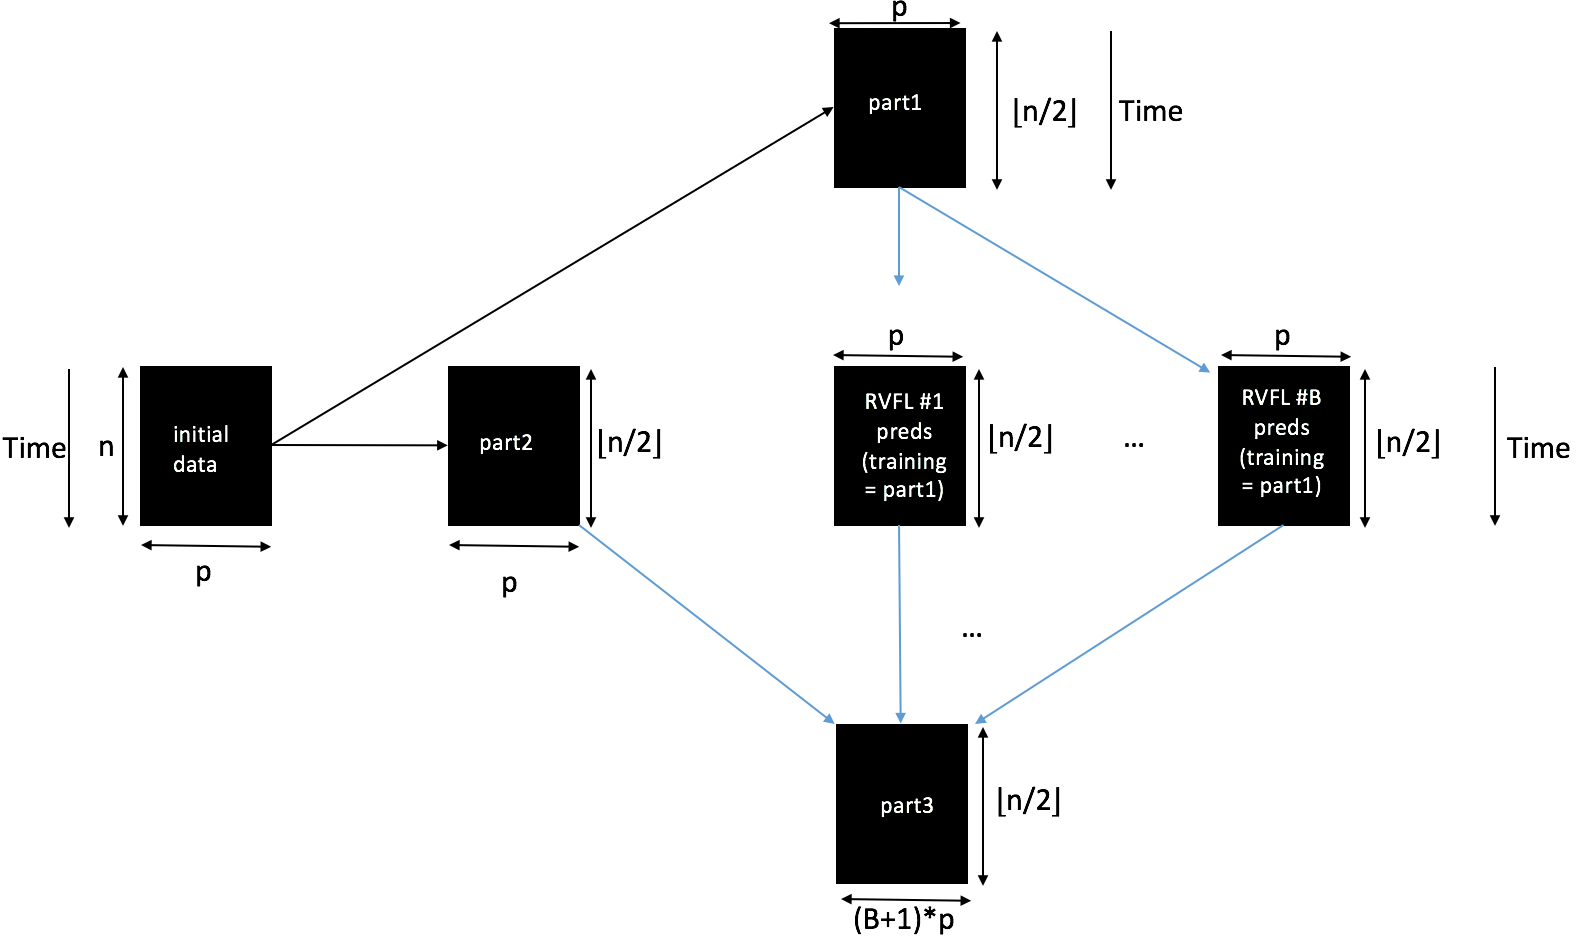
\includegraphics[width=13cm]{gfx/chapter-rvfl-ensembles/rvfl_stacking.png}
\caption{Construction of the enriched/stacked dataset}
\label{rvfl_stacking_plot}
\end{figure}


\section{Numerical examples}
\label{sec:numericalexamples}

For the numerical examples, we obtain forecast of the Treasury Bill rates among other macroeconomic variables, in a \textit{data-rich} environment. We use data from \cite{greene2000econometric}. Four of the time series are considered: the Treasury Bill rates, the real consumption, the consumer price index, and the real expenditure. They are all observed on a quaterly basis. 

We annualize the last three time series, but keep the Treasury Bill rates unchanged. So that, the four time series are nearly on the same scale.

The out-of-sample Root Mean Squared Error (RMSE) is used as a measure of performance of the different implemented models.

\subsection{Descriptive statistics}

Figure \ref{all_series_plot} presents the resulting time series' data obtained after the few transformations described in the previous paragraph. Table \ref{tab:summary_four_ts} contains a summary of these data, where we can see that the four time series are now nearly expressed in the same scale.

\begin{figure}[!htb]
\centering
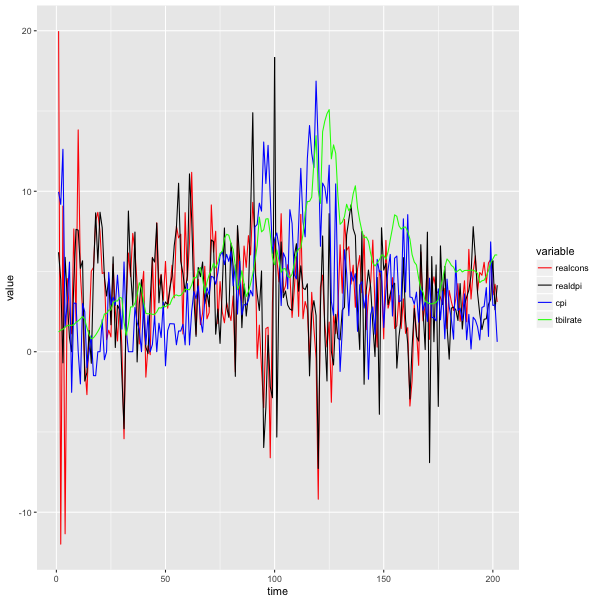
\includegraphics[width=10cm]{gfx/chapter-rvfl-ensembles/all_series.png}
\caption{Treasury Bills rates and transformed Real consumption, Real disposable income, and  Inflation data from \cite{greene2003econometric} in a \textit{data-rich} environment}
\label{all_series_plot}
\end{figure}


\begin{table}[!htb]
\begin{center}
% table caption is above the table
\caption{Summary statistics for the four transformed time series: Treasury Bills and transformed Real consumption, Real disposable income, and  Inflation data from \cite{greene2003econometric}}
\label{tab:summary_four_ts}       % Give a unique label
% For LaTeX tables use
\begin{tabular}{llllllll}
\hline\noalign{\smallskip}
Series & Min & 1st Qrt  & Median  & Mean & 3rd Qrt  & Max & Std. Dev.\\
\noalign{\smallskip}\hline\noalign{\smallskip}
  Real consumption  & -11.990 & 1.814 & 3.637 & \textbf{3.513} & 5.414 & 19.978 & \textbf{3.546}\\
  Real disposable income  & -7.275 & 1.613 & 3.390 & \textbf{3.423} & 5.518 & 18.358 & \textbf{3.486}\\
  Inflation & -2.530  & 1.755 & 3.135 & \textbf{3.936} & 5.593 & 16.864 & \textbf{3.407}\\
  Treasury Bills rates & 0.810  & 3.138 & 5.050 & \textbf{5.270} & 6.715 & 15.090 & \textbf{2.829} \\
\noalign{\smallskip}\hline
\end{tabular}
\end{center}
\end{table}


\begin{table}
\begin{center}
% table caption is above the table
\caption{\textbf{Box-Pierce test for the independence} in the time series observations}
\label{tab:boxpierce}       % Give a unique label
% For LaTeX tables use
\begin{tabular}{llllll}
\hline\noalign{\smallskip}
Series &  \code{X-squared} & \code{p-value}  \\
\noalign{\smallskip}\hline\noalign{\smallskip}
  Real consumption & 0.0133 & \textbf{0.9082}  \\
  Real disposable income & 1.3912 & \textbf{0.2382} \\
  Inflation & 86.428 &  2.2e-16 \\
  Treasury Bills rates & 186.35 & 2.2e-16 \\
\noalign{\smallskip}\hline
\end{tabular}
\end{center}
\end{table}

\begin{figure}[!htb]
\centering
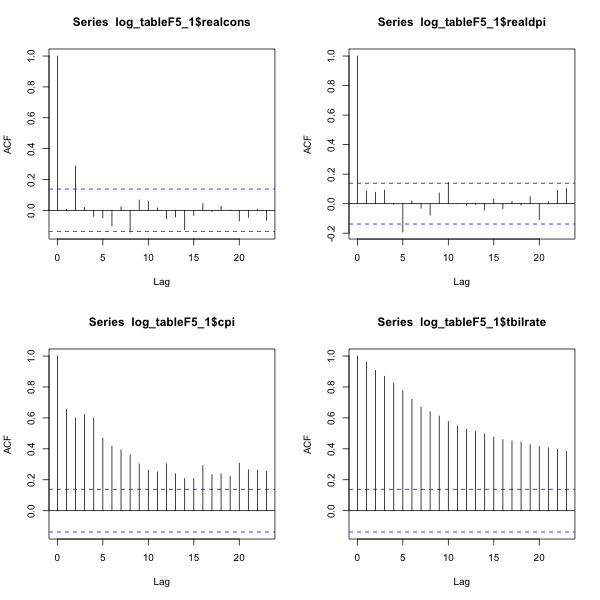
\includegraphics[width=12cm]{gfx/chapter-rvfl-ensembles/acf.png}
\caption{Autocorrelation function for the four times series: Treasury Bills rates, Real consumption, Real disposable income, Inflation}
\label{acf}
\end{figure}

\newpage

The Box-Pierce tests (\cite{box1970distribution}, \cite{ljung1978measure}, \cite{harvey1993time}) results presented in table \ref{tab:boxpierce}, and the autocorrelation functions presented in \ref{acf}, show that the two time series for Real consumption and Real disposable income could be considered as stationary after the transformations. Whereas for the Treasury Bills rates and Inflation, there is still a non-negligible autocorrelation within the series. 

\medskip

Another interesting information is given by figure \ref{corrplot}. We observe that the distribution of the data for inflation and Treasury Bills rates is skewed, when compared to the data for Real consumption and Real disposable income. 

\medskip

Also, based on the correlations displayed in figure \ref{corrplot}, the Real consumption is globally  decreasing when the Treasury Bills rates and the inflation are increasing. But when the Real disposable income increases, the Real consumption increases as well. 

\begin{figure}[!htb]
\centering
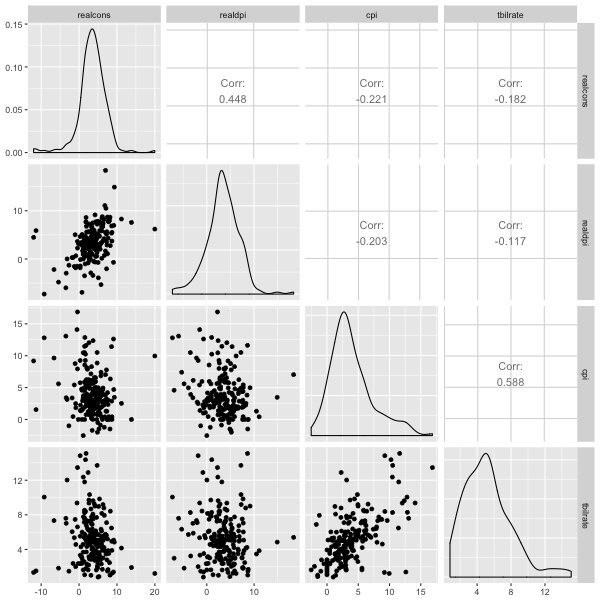
\includegraphics[width=14cm]{gfx/chapter-rvfl-ensembles/scatterplot.png}
\caption{Correlation plot for the four times series: Treasury Bills rates, Real consumption, Real disposable income, Inflation}
\label{corrplot}
\end{figure}

%\newpage

In section \ref{results_summary}, we apply the bagging and stacking procedures described in sections \ref{sec:rvflbagging} and \ref{sec:rvflstacking} to the dataset we have just described. 


A rolling forecasting cross-validation method (see \cite{bergmeir2015note} and figure \ref{rolling_cv}). At the beginning of the procedure, the training set contains $24$ points ($4$ years), and the test set contains $4$ points ($1$ year) and $8$ points ($2$ years). The training set is then advanced of one point forward (rolled), and the procedure is repeated until no more data for the training set are found.  

\begin{figure}[!htb]
\centering
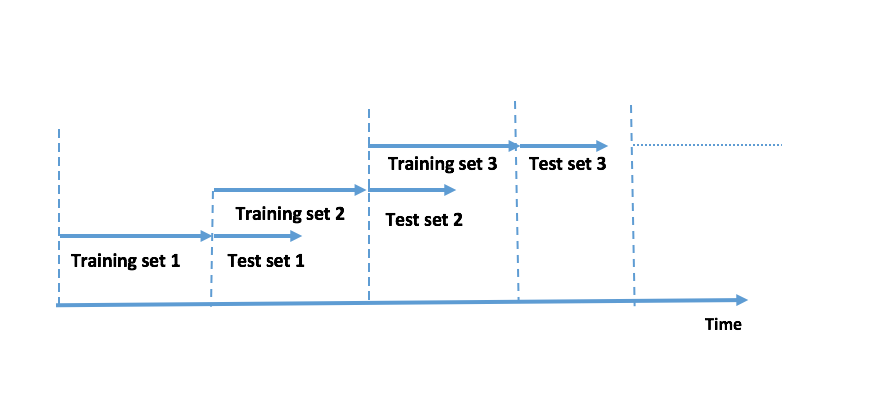
\includegraphics[width=14cm]{gfx/chapter-rvfl-ensembles/rolling_cv.png}
\caption{Training and testing sets in rolling forecasting cross-validation}
\label{rolling_cv}
\end{figure}

As we said at the beginning of section \ref{sec:numericalexamples}, we use the Root Mean Squared Error (RMSE) as a measure of the out-of-sample error. All the benchmarks are made on what is defined as \code{part3} in section \ref{sec:rvflstacking}, in order to have a similar perimeter for bagging and stacking. The results obtained by the ensemble learners are compared to those obtained by the base RVFL model, which are presented here: 

For the bagging example, we use $B = 100$ resamples of the data, and calculate the average out-of-sample RMSE obtained by the ensemble model on all the testing sets (see figure \ref{rolling_cv}). The dataset used, is the one defined as \code{part3} in section \ref{sec:rvflstacking}.  

For the boosting example, we use $B = 10$ boosting iterations of the least squares regression model from formula ~\ref{eq:rvflequation}. The tuning parameters are the learning rate of the boosting algorithm denoted as $\nu$, the number of nodes in the hidden layer for the base-learner \code{nb\underline{  }hidden}, the fraction of the initial time series considered as predictors \code{col\underline{  }sample}, the number of lags. 

For the stacking example, The dataset used, is also the one defined as \code{part3} in section \ref{sec:rvflstacking}. The tuning parameters are the number of boostrap resamples, $B$, and the hyperparameter of the ridge regression model is the regularization parameter. 

\subsection{Summary of results}
\label{results_summary}

A summary of the out-of-sample RMSE is presented in figure \ref{boxplot_perfs} in a logarithmic scale, for all the methods that we described and tested in the previous sections. The numerical values corresponding to these boxplots can be found in appendix \ref{boxplot_summary}, in their original scale. 

The base RVFL model is denoted as \code{ridge2}. \code{bagging}, \code{stack\underline{  }ridge}, \code{stack\underline{  }lm}, \code{stack\underline{  }nnls}, and \code{glmboost} respectively denote the bootstrap aggregating method from section \ref{sec:rvflbagging}, stacking with ridge regression, with ordinary least squares, least squares regression with positive coefficients from section \ref{sec:rvflstacking}, and boosting from section \ref{sec:rvflboosting}. We also added an unrestricted Vector AutoRegression (VAR) model to the benchmarks, denoted as \code{VAR}, which mostly helps us in assessing if the other models' implementation/predictions are not off track.  

\begin{figure}[!htb]
\centering
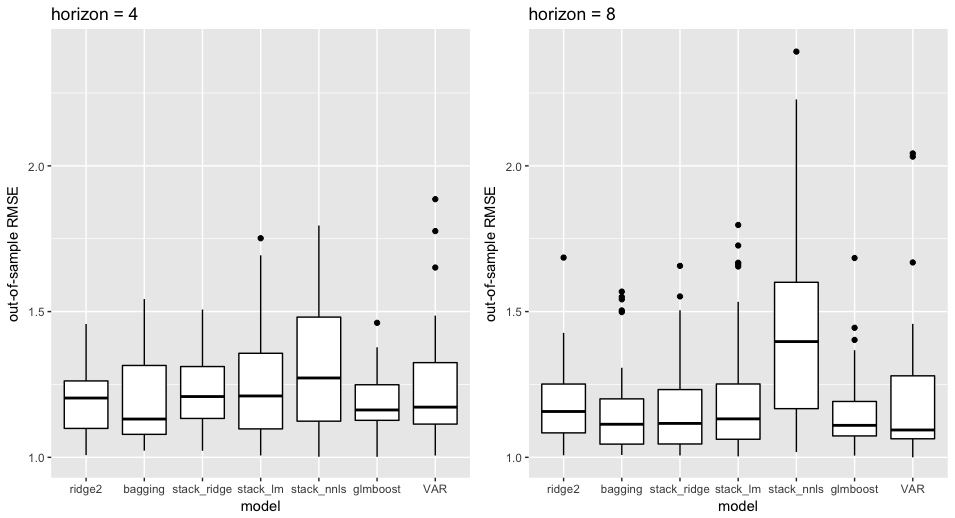
\includegraphics[width=14cm]{gfx/chapter-rvfl-ensembles/boxplot_perfs.png}
\caption{Out-of-sample RMSE distribution for the different tested models}
\label{boxplot_perfs}
\end{figure}

Bagging is performing the best on average (cf. appendix \ref{boxplot_perfs} for details) on both horizons, 4-steps ahead and 8-steps ahead, and is followed by boosting. The stacking algorithm works best with the ridge regression model taken as a meta-learner, but is failing with the other meta learners (ordinary least squares and least squares regression with positive coefficients). Overall, the boosting algorithm is also very robust, and displays the lowest standard deviation of all the models tested. 

The \textit{best} hyperparameters obtained for each algorithm are presented below, for the different horizons of projection. The best hyperparameter found for stacking with ordinary least squares, with a constraint on the regression parameters or not, is the number of lags equal to $1$ and $B = 1$. 

\textbf{For horizon = 4}

\begin{table}[!htb]
\begin{center}
% table caption is above the table
\caption{\textit{Best} hyperparameters for the base RVFL}
\label{tab:bestparamsrvfl}       % Give a unique label
% For LaTeX tables use
\begin{tabular}{lllllll}
\hline\noalign{\smallskip}
Method & lags & nodes & $\lambda_1$ & $\lambda_2$ &   &   \\
\noalign{\smallskip}\hline\noalign{\smallskip}
  \textbf{RVFL} & 3 & 100 & 10000 & 100 &  &  \\
\noalign{\smallskip}\hline
\end{tabular}
\end{center}
\end{table}

\begin{table}[!htb]
\begin{center}
% table caption is above the table
\caption{\textit{Best} hyperparameters for the bagging of RVFLs}
\label{tab:bestparamsbagrvfl}       % Give a unique label
% For LaTeX tables use
\begin{tabular}{llllllll}
\hline\noalign{\smallskip}
Method & lags & nodes & $\lambda_1$ & $\lambda_2$ & B  &  col. sample  & row. sample\\
\noalign{\smallskip}\hline\noalign{\smallskip}
  \textbf{Bagging} & 1 & 1 & 21.54435 & 21.54435 & 100 & 0.9 & 0.9\\
\noalign{\smallskip}\hline
\end{tabular}
\end{center}
\end{table}

\begin{table}[!htb]
\begin{center}
% table caption is above the table
\caption{\textit{Best} hyperparameters for the stacking with ridge regression}
\label{tab:bestparamsbagrvfl}       % Give a unique label
% For LaTeX tables use
\begin{tabular}{llllllll}
\hline\noalign{\smallskip}
Method & lags & $\lambda$ & $B$ & col. sample  &  row. sample  \\
\noalign{\smallskip}\hline\noalign{\smallskip}
  \textbf{Stacking (ridge)} & 3 & 21.54435 &  1 & 0.9 & 0.8   \\
\noalign{\smallskip}\hline
\end{tabular}
\end{center}
\end{table}

\begin{table}[!htb]
\begin{center}
% table caption is above the table
\caption{\textit{Best} hyperparameters for the boosting algorithm}
\label{tab:bestparamsbagrvfl}       % Give a unique label
% For LaTeX tables use
\begin{tabular}{llllllll}
\hline\noalign{\smallskip}
Method & lags & nodes & $\nu$ & $B$ & col. sample  &  & \\
\noalign{\smallskip}\hline\noalign{\smallskip}
  \textbf{Boosting} & 3 & 1 & $0.2020798$ & 10 & 1 & & \\
\noalign{\smallskip}\hline
\end{tabular}
\end{center}
\end{table}

\begin{table}[!htb]
\begin{center}
% table caption is above the table
\caption{\textit{Best} hyperparameters for the VAR}
\label{tab:bestparamsvar}       % Give a unique label
% For LaTeX tables use
\begin{tabular}{llllllll}
\hline\noalign{\smallskip}
Method & lags & type of regressor &  &  &  &  & \\
\noalign{\smallskip}\hline\noalign{\smallskip}
  \textbf{VAR} & 1 & const &  & &  & & \\
\noalign{\smallskip}\hline
\end{tabular}
\end{center}
\end{table}


\textbf{For horizon = 8}

\begin{table}[!htb]
\begin{center}
% table caption is above the table
\caption{\textit{Best} hyperparameters for the base RVFL}
\label{tab:bestparamsrvfl}       % Give a unique label
% For LaTeX tables use
\begin{tabular}{lllllll}
\hline\noalign{\smallskip}
Method & lags & nodes & $\lambda_1$ & $\lambda_2$ &   &   \\
\noalign{\smallskip}\hline\noalign{\smallskip}
  \textbf{RVFL} & 3 & 2 & 21.54435 & 10000 &  &  \\
\noalign{\smallskip}\hline
\end{tabular}
\end{center}
\end{table}

\begin{table}[!htb]
\begin{center}
% table caption is above the table
\caption{\textit{Best} hyperparameters for the bagging of RVFLs}
\label{tab:bestparamsbagrvfl}       % Give a unique label
% For LaTeX tables use
\begin{tabular}{llllllll}
\hline\noalign{\smallskip}
Method & lags & nodes & $\lambda_1$ & $\lambda_2$ & B  &  col. sample  & row. sample\\
\noalign{\smallskip}\hline\noalign{\smallskip}
  \textbf{Bagging} & 1 & 1 & 21.54435 & 21.54435 & 100 & 0.9 & 0.9\\
\noalign{\smallskip}\hline
\end{tabular}
\end{center}
\end{table}

\begin{table}[!htb]
\begin{center}
% table caption is above the table
\caption{\textit{Best} hyperparameters for the stacking with ridge regression}
\label{tab:bestparamsbagrvfl}       % Give a unique label
% For LaTeX tables use
\begin{tabular}{llllllll}
\hline\noalign{\smallskip}
Method & lags & $\lambda$ & $B$ & col. sample  &  row. sample  \\
\noalign{\smallskip}\hline\noalign{\smallskip}
  \textbf{Stacking (ridge)} & 3 & 21.54435 &  1 & 0.9 & 0.9   \\
\noalign{\smallskip}\hline
\end{tabular}
\end{center}
\end{table}

\begin{table}[!htb]
\begin{center}
% table caption is above the table
\caption{\textit{Best} hyperparameters for the boosting algorithm}
\label{tab:bestparamsbagrvfl}       % Give a unique label
% For LaTeX tables use
\begin{tabular}{llllllll}
\hline\noalign{\smallskip}
Method & lags & nodes & $\nu$ & $B$ & col. sample  &  & \\
\noalign{\smallskip}\hline\noalign{\smallskip}
  \textbf{Boosting} & 3 & 1 & $0.175$ & 10 & 1 & & \\
\noalign{\smallskip}\hline
\end{tabular}
\end{center}
\end{table}

\begin{table}[!htb]
\begin{center}
% table caption is above the table
\caption{\textit{Best} hyperparameters for the VAR}
\label{tab:bestparamsvar}       % Give a unique label
% For LaTeX tables use
\begin{tabular}{llllllll}
\hline\noalign{\smallskip}
Method & lags & type of regressor &  &  &  &  & \\
\noalign{\smallskip}\hline\noalign{\smallskip}
  \textbf{VAR} & 1 & none &  & &  & & \\
\noalign{\smallskip}\hline
\end{tabular}
\end{center}
\end{table}

\newpage

Below, in figure \ref{oos_rmse_over_time}, we can observe how the different methods perform through time. We observe that the models' errors are highly correlated, which is reassuring concerning their implementation. 

\begin{figure}[!htb]
\centering
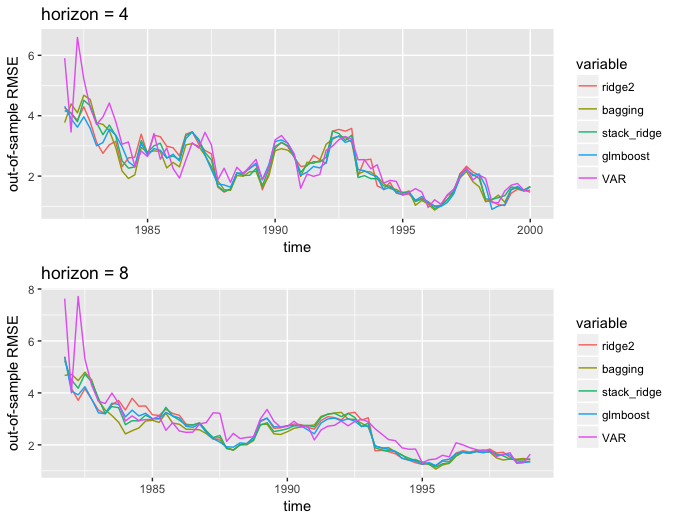
\includegraphics[width=14cm]{gfx/chapter-rvfl-ensembles/oos_rmse_over_time.png}
\caption{Out-of-sample RMSE over time for the different tested models + VAR}
\label{oos_rmse_over_time}
\end{figure}

The details of the correlations between these errors can be found in appendix \ref{oos_errors_cor}. The VAR model generally exhibits a higher variance than the other models (excluding stacking with \code{stack\underline{  }lm} and \code{stack\underline{  }nnls}), but is still able to perform better than them at times (due to the high variance).    

\newpage

\section{Appendix}

\subsection{Out-of-sample errors summary}
\label{boxplot_summary}

\textbf{horizon = 4}

\begin{itemize}

\item Min., 1st Qu., Median, Mean, 3rd Qu., Max

\begin{verbatim}
 ridge2           bagging          stack_ridge      stack_lm         
 Min.   :0.9995   Min.   :0.8746   Min.   :0.9291   Min.   :0.9784   
 1st Qu.:1.5529   1st Qu.:1.5908   1st Qu.:1.6426   1st Qu.:1.7379   
 Median :2.3605   Median :2.1484   Median :2.2407   Median :2.1715      
 Mean   :2.3763   Mean   :2.3034   Mean   :2.3676   Mean   :2.5058      
 3rd Qu.:3.0261   3rd Qu.:2.8957   3rd Qu.:3.0690   3rd Qu.:3.0031      
 Max.   :4.2952   Max.   :4.6781   Max.   :4.5133   Max.   :5.7641
 
 stack_nnls           glmboost          VAR
 Min.   :0.9874       Min.   :0.8996    Min.   :1.041 
 1st Qu.:1.7273       1st Qu.:1.6477    1st Qu.:1.680
 Median :2.2839       Median :2.2443    Median :2.146
 Mean   :2.5115       Mean   :2.3261    Mean   :2.498
 3rd Qu.:3.0494       3rd Qu.:3.0648    3rd Qu.:3.070
 Max.   :6.0210       Max.   :4.3121    Max.   :6.068
\end{verbatim}

\item Standard deviation

\begin{verbatim}
   ridge2   bagging stack_ridge    stack_lm  stack_nnls    glmboost   VAR
0.8804324 0.8881329   0.8870853   1.0549136   1.0889430   0.8238531   1.0511201
\end{verbatim}

\end{itemize}

\textbf{horizon = 8}

\begin{itemize}

\item Min., 1st Qu., Median, Mean, 3rd Qu., Max

\begin{verbatim}
  ridge2         bagging       stack_ridge       stack_lm               
 Min.   :1.192   Min.   :1.066   Min.   :1.143   Min.   :1.253      
 1st Qu.:1.740   1st Qu.:1.717   1st Qu.:1.754   1st Qu.:1.813      
 Median :2.663   Median :2.467   Median :2.656   Median :2.694      
 Mean   :2.529   Mean   :2.440   Mean   :2.509   Mean   :2.676      
 3rd Qu.:3.154   3rd Qu.:2.868   3rd Qu.:3.041   3rd Qu.:3.065      
 Max.   :5.394   Max.   :4.800   Max.   :5.243   Max.   :6.032      
 
 stack_nnls           glmboost          VAR
 Min.   : 1.164       Min.   :1.203     Min.   :1.289
 1st Qu.: 2.056       1st Qu.:1.718     1st Qu.:1.920
 Median : 2.775       Median :2.683     Median :2.648 
 Mean   : 3.331       Mean   :2.478     Mean   :2.696 
 3rd Qu.: 4.069       3rd Qu.:3.024     3rd Qu.:2.964
 Max.   :10.935       Max.   :5.387     Max.   :7.711
\end{verbatim}

\item Standard deviation

\begin{verbatim}
   ridge2     bagging stack_ridge    stack_lm  stack_nnls    glmboost         VAR
0.8955453   0.8883188   0.9093582   1.0406195   1.8865643   0.8547240   1.1482777 
\end{verbatim}

\end{itemize}

\subsection{Correlation of out-of-sample errors}
\label{oos_errors_cor}

\textbf{horizon = 4}

\begin{verbatim}
            ridge2   bagging      stack_ridge  glmboost       VAR
ridge2      1.0000000 0.9350414   0.9658978    0.9627834      0.8422500
bagging     0.9350414 1.0000000   0.9796091    0.9388819      0.8746823
stack_ridge 0.9658978 0.9796091   1.0000000    0.9731609      0.8758017
glmboost    0.9627834 0.9388819   0.9731609    1.0000000      0.8840573
VAR         0.8422500 0.8746823   0.8758017    0.8840573      1.0000000
\end{verbatim}

\textbf{horizon = 8}

\begin{verbatim}
                ridge2  bagging stack_ridge  glmboost       VAR
ridge2      1.0000000 0.9280983   0.9693424 0.9909838 0.8185879
bagging     0.9280983 1.0000000   0.9855720 0.9481774 0.8522099
stack_ridge 0.9693424 0.9855720   1.0000000 0.9804522 0.8561227
glmboost    0.9909838 0.9481774   0.9804522 1.0000000 0.8622763
VAR         0.8185879 0.8522099   0.8561227 0.8622763 1.0000000
\end{verbatim} % INCLUDE: rvfl-ensembles
\cleardoublepage
>>>>>>> chapter-4-rvfl-ensembles

%\forcenewpage

%% !TEX root = ../thesis-example.tex
%
\chapter{Conclusion}
\label{sec:conclusion}

 % INCLUDE: conclusion
%\cleardoublepage

% --------------------------
% Back matter
% --------------------------
{%
\setstretch{1.1}
\renewcommand{\bibfont}{\normalfont\small}
\setlength{\biblabelsep}{0pt}
\setlength{\bibitemsep}{0.5\baselineskip plus 0.5\baselineskip}
\printbibliography[nottype=online]
\printbibliography[heading=subbibliography,title={Webseiten},type=online,prefixnumbers={@}]
}
\cleardoublepage

\listoffigures
\cleardoublepage

\listoftables
\cleardoublepage

% !TEX root = ../thesis-example.tex
%
\pagestyle{empty}
\hfill
\vfill
\pdfbookmark[0]{Colophon}{Colophon}
\section*{Colophon}

This thesis was typeset with \LaTeXe.
It uses the \textit{Clean Thesis} style developed by Ricardo Langner.
The design of the \textit{Clean Thesis} style is inspired by user guide documents from Apple Inc.

Download the \textit{Clean Thesis} style at \url{http://cleanthesis.der-ric.de/}.

\cleardoublepage

% !TEX root = ../thesis-example.tex
%
%************************************************
% Declaration
%************************************************
\pdfbookmark[0]{Declaration}{Declaration}
\chapter*{Declaration}
\label{sec:declaration}
\thispagestyle{empty}

You can put your declaration here, to declare that you have completed your work solely and only with the help of the references you mentioned.

\bigskip

\noindent\textit{\thesisUniversityCity, \thesisDate}

\smallskip

\begin{flushright}
	\begin{minipage}{5cm}
		\rule{\textwidth}{1pt}
		\centering\thesisName
	\end{minipage}
\end{flushright}

%*****************************************
%*****************************************

\clearpage
\newpage
\mbox{}

% **************************************************
% End of Document CONTENT
% **************************************************
\end{document}
